% IEEE PacificVis 2027 -- Conference Paper Track. VGTC conference template (2024.02.14).
% Compile with pdfLaTeX + BibTeX (e.g., upload the folder to Overleaf).
% Experiment entry points and result provenance are documented in README.md.
% Full derivations are included in supplement_proofs.tex.

\documentclass[review]{vgtc}                 % review version (double blind)
%\documentclass{vgtc}                         % final (conference style)

\usepackage{iftex}
\usepackage{graphicx}
\ifPDFTeX
  \pdfoutput=1\relax
  \pdfcompresslevel=9
  \pdfoptionpdfminorversion=7
\fi%
\DeclareGraphicsExtensions{.pdf,.png,.jpg,.jpeg,.eps}

\usepackage[T1]{fontenc}
\usepackage{times}
\renewcommand*\ttdefault{txtt}
\usepackage{booktabs}
\usepackage{flushend}
\usepackage{placeins}
\usepackage{multirow,colortbl}
\setcounter{dbltopnumber}{2}
\renewcommand{\dbltopfraction}{0.9}
\renewcommand{\topfraction}{0.9}
\renewcommand{\bottomfraction}{0.8}
\renewcommand{\textfraction}{0.08}
\renewcommand{\floatpagefraction}{0.85}
\renewcommand{\dblfloatpagefraction}{0.85}
\setlength{\textfloatsep}{10pt plus 2pt minus 2pt}
\setlength{\dbltextfloatsep}{10pt plus 2pt minus 2pt}
\usepackage{mathptmx}
\usepackage{cite} % ascending numeric citations, as required by VGTC
\usepackage{amsmath,amssymb,amsthm}
\usepackage{algorithm}
\usepackage[noend]{algpseudocode}
% vgtcinsertpkg loads xcolor with svgnames; do not load it without options first.
\newtheorem{lemma}{Lemma}
\newtheorem{theorem}{Theorem}
\newtheorem{proposition}[theorem]{Proposition}
\newtheorem{corollary}[theorem]{Corollary}
\newtheorem{definition}[theorem]{Definition}
\newcommand{\free}{\mathrm{free}}
\newcommand{\dtop}{d_{\mathrm{top}}}
\newcommand{\lca}{\operatorname{lca}}


\title{Reference-Guided Merge Tree Maps:\\Quantifying Position--Topology Trade-offs}
\author{Anonymous Authors}\onlineid{0}\vgtccategory{Research}\vgtcinsertpkg
\hypersetup{pdftitle={Reference-Guided Merge Tree Maps: Quantifying Position--Topology Trade-offs}}
\abstract{
Merge tree maps summarize scalar fields through a hierarchy of extrema and their merge relations. Keeping each subtree contiguous can displace features from their projected spatial positions. We present Reference-Guided Merge Tree Maps (RG-MTM), which diagnoses this conflict and constructs maps with an explicit position--topology trade-off. A positional certificate separates interval-packing cost from the additional displacement imposed by hierarchy. Optimal scalar filling for a fixed leaf order preserves extremum values and minimizes labelled pairwise merge-level error, yielding exact attainable frontiers for small trees. RG-MTM-P preserves source merge levels; RG-MTM-R selectively releases contiguity constraints and reports the resulting scalar cost. Across four real temporal sequences and one synthetic sequence comprising 614 frames, both modes improve reference order over shared-input TMTM and ST-MTM baselines. On Storms, the 20\% eligibility setting (R20) reduces P's order error from 3.77\% to 1.16\%, with 1.47\% mean merge-level error; its motion-proxy errors decrease to 19/104 from ST-MTM's 43/104. Independent experiments cover Tangaroa (201 original-grid volumes), Cylinder (102 volumes), one static Nucleon slice, and 21 reconstructed Benzene potential sections. On Tangaroa, R20 reduces P's order error from 9.61\% to 0.019\%, at 14.44\% mean merge-level error. These results quantify the reference alignment gained and scalar connectivity changed by a chosen order, while retaining the source fields for spatial interpretation.
}
\keywords{Temporal scalar fields, merge tree maps, reference-guided layout, positional certificates, merge-level distortion.}
\teaser{
\centering
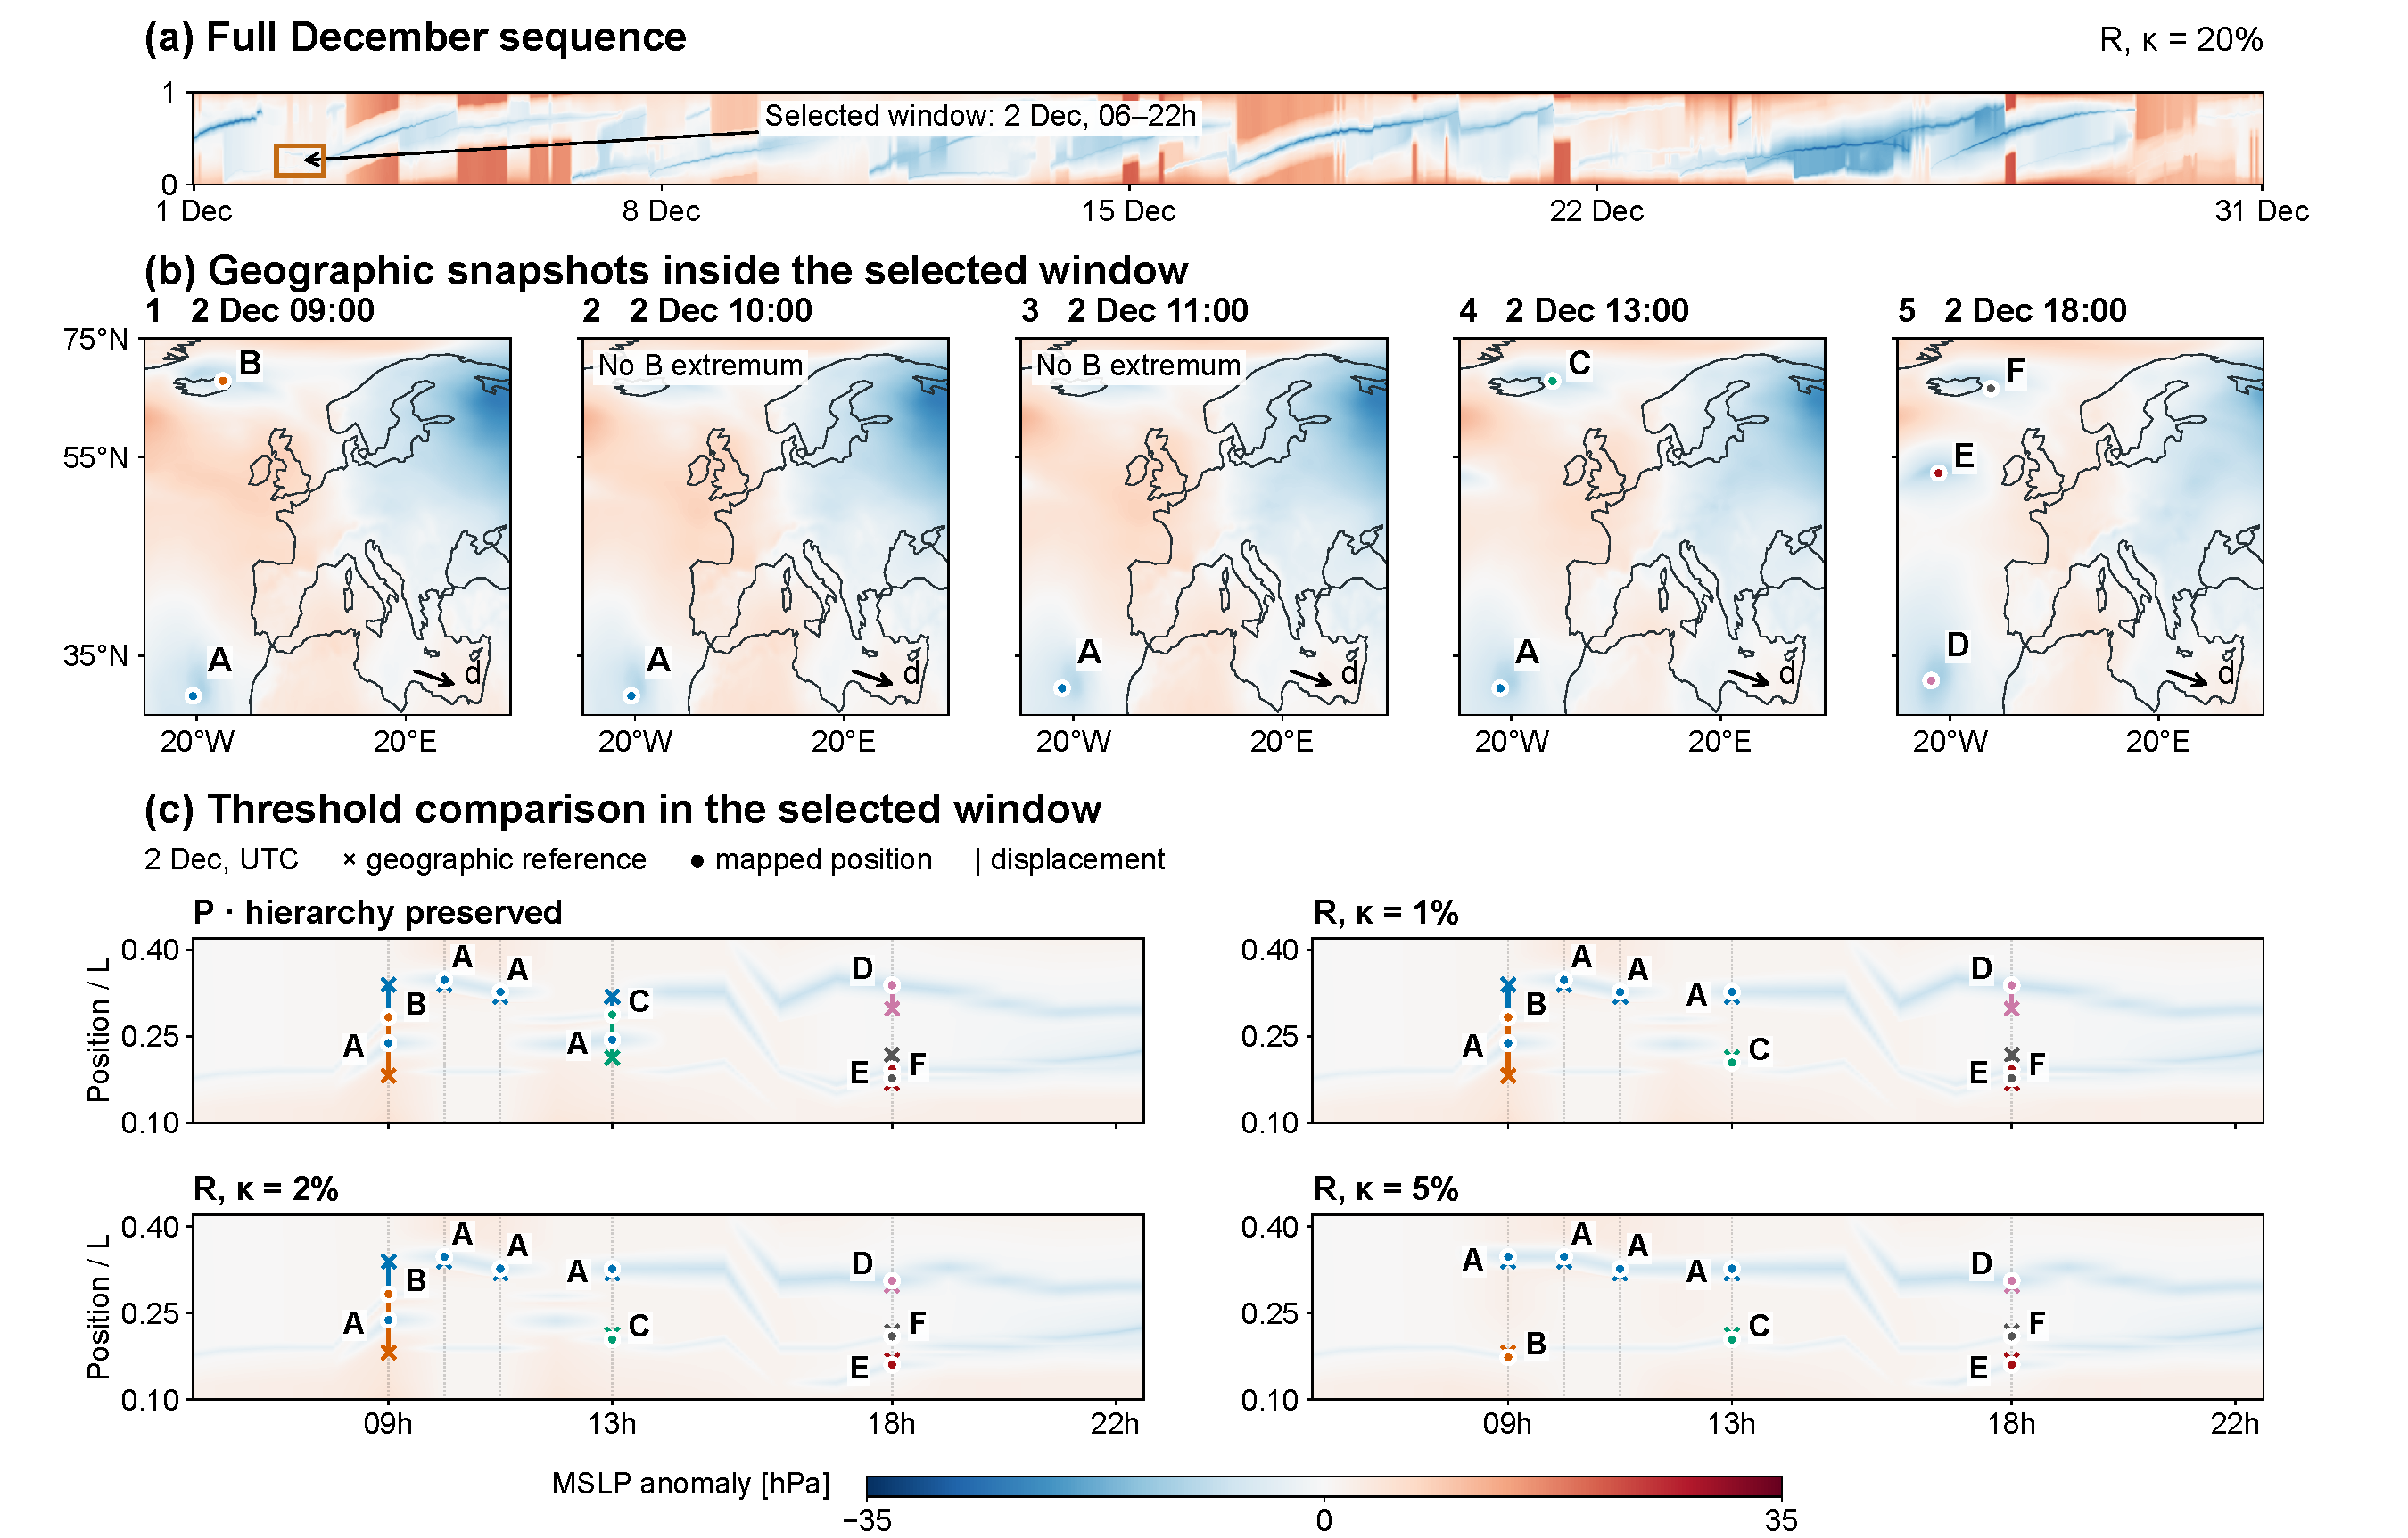
\includegraphics[width=\linewidth]{figures/Fig1.pdf}
\par\smallskip\refstepcounter{figure}\label{fig:teaser}
{\captionfonts\noindent\figurename~\thefigure: RG-MTM-R20 visualization of hourly Storms pressure anomalies over December 1999. (a) All 744 hourly fields are mapped along the data-derived fixed direction $d\approx(0.948,-0.319)$ and linked to five source snapshots. Blue and red encode negative and positive anomalies on a shared $[-35,35]$\,hPa scale. Event names and times follow TMTM~\cite{Koepp:2023:TMTM}; labels identify computed extrema near the reported regions rather than independently validated cyclone tracks. The red dashed outline selects all of 26 December. (b) The 10:00 source field marks $A=130$, $B=113$, and $C=133$; the lower map retains all 24 hourly profiles over the full $[0,1]$ output axis. Solid curves show saved anchors over 00:00--23:00 UTC, with gaps outside saved lifetimes; $C$ exists only from 05:00 to 10:00. Anomalies subtract a centered 192-hour mean; layout uses the RG-MTM $49\times49$ grid and 250\,km smoothing. Display interpolation preserves each hourly profile. This visualization is independent of the 118-frame Storms quantitative evaluation.\par}
}

\begin{document}
\firstsection{Introduction}
\maketitle
\raggedbottom
\setlength{\emergencystretch}{1em}
Time-varying scalar fields describe pressure, fire activity, radiation, pollution, and simulated flow. Their extrema identify intensity regions; merge levels record when these regions connect. Static temporal summaries expose feature strength, lifetime, and connectivity across distant time steps.

Temporal merge tree maps (TMTM) linearize each field through its augmented merge tree and align consecutive profiles through subtree overlap~\cite{Koepp:2023:TMTM}. Spatiotemporal merge tree maps (ST-MTM) introduce a distance-aware one-dimensional skeleton and temporal coherence~\cite{STMTM:2026}. Both generate orders by recursively arranging complete child subtrees. This keeps hierarchical features together, but the resulting axis follows tree connectivity rather than a fixed spatial coordinate.

The distinction matters when position is part of the analysis. The frame-48 Storms case in Supplement S8 exposes this conflict: the source tree groups $A,B$, while $C$ lies between their reference positions along the selected direction. Keeping $A,B$ contiguous excludes their geographic order: at least one feature must move away from its reference position. Admitting that order instead changes the scalar barriers representing their merge relations. The choice concerns both spatial alignment and the pressure threshold at which structures connect.

We ask \textbf{RQ1}: when hierarchy must be preserved, why is reference displacement unavoidable, and how small can it be? \textbf{RQ2}: which hierarchy constraints can be released to improve alignment, and what merge-level change does the resulting map incur? \textbf{Reference-Guided Merge Tree Maps (RG-MTM)} uses a fixed spatial projection as its target. It diagnoses unavoidable displacement before layout, then constructs either a preserving map, RG-MTM-P, or a selectively relaxed map, RG-MTM-R. Both retain the extrema and their values; the relaxed map reports the change in their pairwise merge levels.

Our evaluation also asks \textbf{RQ3}: how do these choices affect reference alignment, scalar connectivity, and motion proxies across temporal, static, and volumetric inputs?

The paper makes three contributions:
\begin{itemize}
\item A positional certificate that separates interval-packing and hierarchy costs, together with conflict triples that identify the obstructing feature relations.
\item An optimal fixed-order barrier construction and exact small-tree position--topology frontiers, connecting a changed leaf order to its minimum scalar cost.
\item A reference-guided construction connecting diagnosis, hierarchy selection, interval layout, and scalar filling, evaluated on five planar temporal sequences, an independent reference-position control, two original-grid volumetric sequences, and static Nucleon and reconstructed Benzene inputs.
\end{itemize}
The evaluation measures reference order, achieved anchor displacement, rendered merge levels, and approach/separation decisions. Source fields, temporal maps, and error records connect these measurements to the feature relations changed by each mode. Sections~\ref{sec:model}--\ref{sec:analysis} establish the model and its guarantees; Section~\ref{sec:method} describes the construction. Section~\ref{sec:eval} tests the mechanisms and shared-input comparisons, Section~\ref{sec:results} examines source-linked results by spatial dimension, and Section~\ref{sec:discussion} discusses interpretation and limits.

\section{Related Work}
\paragraph{Temporal summaries and spatial linearization.}
Generalized space--time cubes describe temporal visualizations through transformations of space and time~\cite{Bach:2017:STC}. Studies of animation and trend analysis show how presentation and comparison tasks affect the usefulness of animated and static displays~\cite{Tversky:2002:Animation,Robertson:2008:Animation}. Static temporal maps place distant time steps in one view, with their interpretation determined by the compressed spatial axis. Hovm\"oller diagrams retain a selected spatial coordinate~\cite{Hovmoller:1949}; geographic orderings and context-based space-filling curves construct spatial traversals~\cite{Guo:2006:SpatialOrder,Dafner:2000:CSFC}. Dynamic Volume Lines apply space-filling traversals to volumetric comparison~\cite{Weissenboeck:2019:DVL}, while one-dimensional projections and data-driven curves adapt the ordering to spatiotemporal fields~\cite{Franke:2021:1DP,Zhou:2021:DSF}. MotionRugs instead organize moving point features~\cite{Buchmueller:2019:MR}. RG-MTM gives the axis a fixed projection target and quantifies the displacement introduced by hierarchical feature grouping.

\paragraph{Feature tracking and evolving hierarchies.}
Feature tracking connects spatial structures across time, including evolving regions and turbulent three-dimensional features~\cite{Samtaney:1994:Tracking,Silver:1997:Tracking}. Topology-based approaches organize such correspondences through multiscale structures, global scalar-feature matching, and time-varying merge trees~\cite{Bremer:2010:Burning,Saikia:2017:GFT,Oesterling:2017:TVMT}. Dynamic tracking graphs support exploration of temporal relationships~\cite{Widanagamaachchi:2012:DTG}; nested and dynamic nested tracking graphs add the hierarchical relationships of scalar features~\cite{Lukasczyk:2017:NTG,Lukasczyk:2020:DNTG}. Temporal Treemaps summarize evolving trees as time-aligned bands~\cite{Koepp:2019:TT}, and Fuzzy Contour Trees align multiple trees in a joint layout~\cite{Lohfink:2020:FCT}. These methods establish feature identity and hierarchical context across observations. RG-MTM uses support-overlap matches as input and addresses the subsequent placement of matched extrema against a fixed reference.

\paragraph{Topology-based scalar maps.}
Topological landscapes represent scalar connectivity through terrain, with geometry-preserving extensions introducing proximity between features~\cite{Weber:2007:TL,Beketayev:2012:GPTL}. TMTM traverses augmented merge trees to keep features intact and optimizes subtree overlap between adjacent time steps~\cite{Koepp:2023:TMTM}. ST-MTM separates a hierarchy-constrained skeleton from leaf-arc and path filling, improving geometric distances and temporal coherence~\cite{STMTM:2026}. Section~\ref{sec:prior_pipelines} and Fig.~\ref{fig:prior_work} summarize both workflows before defining our reference-guided extension. RG-MTM reuses this scalar/path filling and separates the original tree, which supplies merge targets, from the ordering tree, which specifies admissible permutations. Pairwise distances can remain unchanged under a global translation or reflection, whereas fixed-reference residuals detect either transformation. RG-MTM therefore adds an absolute positional target to the geometry-aware design space. Its certificate measures the reference-position obstruction, and its scalar correction minimizes merge-level error for the selected order and fixed extremum values.

\paragraph{Ordering, simplification, and tree comparison.}
Optimal leaf ordering searches tree-consistent permutations~\cite{BarJoseph:2001:OLO}. Separation-constrained layout and interval separation control overlap and displacement~\cite{Dwyer:2006:IPSEP,Li:2019:SOI}. RG-MTM couples these constraints with reference coordinates, interval widths, and anchor slack. Persistence simplification removes scalar features~\cite{Edelsbrunner:2002:TPS,Tierny:2012:GTS}; our ordering relaxation retains the leaves and releases selected contiguity constraints. Topological comparison methods span several descriptors and matching assumptions~\cite{Yan:2021:Survey}, including labelled cophenetic/interleaving comparisons~\cite{Munch:2019:LINF,Yan:2022:GAMT}, Wasserstein merge-tree comparisons~\cite{Pont:2022:WMT}, and branch-decomposition-independent edit distances~\cite{Wetzels:2022:BDI}. Our discrepancy uses fixed leaf correspondences to measure the scalar change introduced by an order and its filled profile.

\paragraph{Layout quality.}
Stress and trustworthiness assess distance and neighbourhood preservation~\cite{Smelser:2025:Scale,Venna:2001:NP,Nonato:2019:MP}; ST-MTM also evaluates temporal displacement~\cite{STMTM:2026}. We combine these measures with reference-order error, actual anchor displacement, and rendered merge-level error, distinguishing the spatial, temporal, and topological properties represented by the map.

\section{Background and Problem Formulation}\label{sec:model}
\subsection{From Augmented Trees to Temporal Maps}\label{sec:prior_pipelines}
\begin{figure}[H]
\centering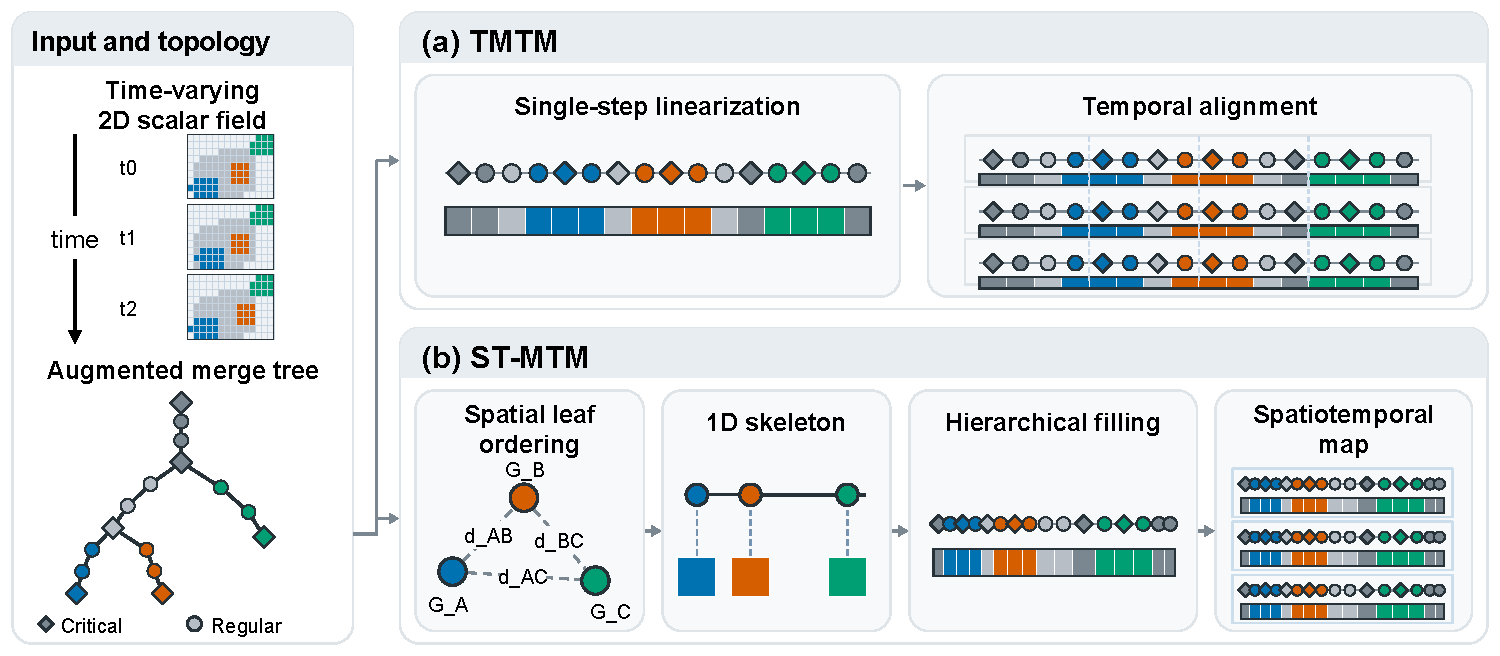
\includegraphics[width=\linewidth]{figures/Fig2.pdf}
\caption{Conceptual comparison of preceding merge-tree map workflows, redrawn and extended from ST-MTM Figs.~1 and 3~\cite{STMTM:2026}. Both use augmented trees with critical (diamond) and regular (circle) nodes. (a) TMTM~\cite{Koepp:2023:TMTM} linearizes samples within subtrees and optimizes temporal alignment. (b) ST-MTM constructs a distance-aware 1D skeleton, fills its scalar domain, and assembles the map. Branch/sample identities use the same palette throughout the schematics: $A$ (blue), $B$ (orange), and $C$ (green); internal groups are grey.}
\label{fig:prior_work}
\end{figure}

Figure~\ref{fig:prior_work} summarizes the two constructions on which RG-MTM builds. Both start from an augmented merge tree for each scalar-field observation. Critical nodes describe extrema and component merges; regular nodes retain samples along the arcs. The branching hierarchy groups connected scalar regions, while augmentation carries their values into the linearized field.

In TMTM, a recursive traversal maps all tree samples to a one-dimensional profile~\cite{Koepp:2023:TMTM}. Each subtree occupies a contiguous interval whose length is proportional to its sample count. Changing child order changes the linearization while preserving the merge tree. Temporal optimization selects these branch decisions to make interval overlaps between adjacent profiles agree with source-space subtree overlaps; stacking the aligned profiles produces the temporal map (Fig.~\ref{fig:prior_work}(a)).

ST-MTM separates geometric layout from scalar filling~\cite{STMTM:2026}. It first reorders leaves within the hierarchy using distances between feature centroids, then optimizes a one-dimensional skeleton to approximate feature distances under non-overlap constraints. Its temporal mode also uses tracked leaves to improve consistency between consecutive layouts. Leaf-arc sampling and hierarchical path filling populate the resulting intervals and gaps with scalar values before temporal assembly (Fig.~\ref{fig:prior_work}(b)). The diagram's lower path summarizes these stages; its temporal optimization acts during skeleton construction.

These constructions establish topology-preserving linearization and geometry-aware placement, respectively. Their admissible orders keep each subtree contiguous. A fixed spatial projection can instead request interleaved leaves from different subtrees, making reference alignment incompatible with that order constraint. RG-MTM diagnoses the resulting displacement, selects which constraints to retain or release, and measures the scalar cost of the chosen order. It reuses the augmented trees and scalar/path-filling framework while adding reference coordinates, positional certificates, and optimal barrier correction.

\subsection{Scalar Features and Merge Relations}
The input comprises processed fields $F_t:\Omega\rightarrow\mathbb R$, augmented merge trees $T_t$, leaf supports, and temporal matches. For a join tree, leaves are minima and internal nodes record the levels at which sublevel-set components merge. Split trees follow the same convention after negating scalar values. Augmentation retains regular samples along tree arcs, providing field context for the one-dimensional profile.

Leaf $i$ has extremum position $e_i^t$, value $f_t(i)$, support measure $\mu_i^t$, and support centroid $G_i^t$. The measure is area for a planar field and volume for a volumetric field. The extremum defines the positional reference; the centroid supplies the geometric distance term. Adjacent-frame support intersections define a maximum-weight Hungarian matching, with positive-overlap assignments continued as tracks.

Contracting unary chains gives the branching hierarchy for ordering. A legal permutation $\pi\in\Pi(T)$ keeps every subtree's leaves contiguous. For a join profile $\psi$, the merge level of two labelled extrema is the maximum on their inter-anchor interval $I_{ij}$. Its discrepancy from the source tree is
\begin{equation}
 d_{\rm top}(\psi,T)=\max_{i<j}\left|\max_{x\in I_{ij}}\psi(x)-f(\lca_T(i,j))\right|.
 \label{eq:merge_error}
\end{equation}
The original tree $T$ defines these targets; the ordering tree $T'$ defines admissible permutations; the filled profile $\psi$ is the measured output. A single-leaf frame has zero pairwise error.

\subsection{Reference Positions and Interval Geometry}
A fixed projection assigns $q_i^t=\langle e_i^t,d\rangle$ to one canvas $[a,a+L]$. Each feature receives a width $w_i=c\mu_i$, interval centre $z_i$, and extremum anchor $u_i$. Its eccentricity radius is $h_i=\rho w_i/2$. The interval must lie inside the canvas, consecutive intervals must leave a gap of at least $g$, and the anchor must remain within $h_i$ of its centre. Together these rules define the interval geometry $\mathcal G$ used by Algorithm~\ref{alg:rgmtm} and the layout in Section~\ref{sec:method}.

The width scale $c$, gap $g>0$, slack fraction $0\le\rho\le1$, and canvas remain fixed across time. Packing requires $\sum_iw_i+(n-1)g\le L$. Positive gaps separate the ordered anchors while allowing motion within their allocated intervals. Supplement S1 gives the complete linear constraints.

The primary position objective minimizes $\max_i|u_i-q_i|$. The scalar objective minimizes Equation~\eqref{eq:merge_error} with fixed extremum values. Temporal layout follows the projected displacement of matched extrema. These objectives connect source coordinates, scalar connectivity, and temporal evolution within one explicit display model.

\section{A Unified Position--Topology Framework}\label{sec:framework}
We formulate topology preservation, geometric fidelity, temporal alignment and reference guidance within one interval representation. The variables, geometry, solver and scalar renderer remain the same across operating regimes. Parameters change which relations matter and which errors are permitted. TMTM-inspired and ST-MTM-inspired regimes express prior design principles; they do not replace the independently implemented native baselines.

\subsection{One Layout Objective}
At frame $t$, the variables are leaf order $\pi_t$, anchors $u_t$, interval centres $z_t$, and inter-anchor barriers $b_t$. Widths $w_i=c\mu_i$, canvas $[a,a+L]$, source merge targets and scalar range $\Delta_F$ are shared across regimes. Let $\mathcal M_t$ contain matched leaves, $p_i$ their preceding displayed positions, $\Delta q_i=q_i^t-q_i^{t-1}$, and $d_{ij}=\|G_i^t-G_j^t\|$. Define
\begin{equation}
\begin{aligned}
 E_R &= \frac{1}{n_tL^2}\sum_i(u_i-q_i)^2,\\
 E_G &= \frac{1}{N_tL^2}\sum_{i<j}(|u_j-u_i|-d_{ij})^2,\\
 E_M(\eta) &= \frac{1}{|\mathcal M_t|L^2}\sum_{i\in\mathcal M_t}(u_i-p_i-\eta\Delta q_i)^2,\\
 E_C &= \frac{1}{n_tL^2}\sum_i(u_i-z_i)^2,
\end{aligned}\label{eq:unified_terms}
\end{equation}
where $N_t=\binom{n_t}{2}$. A term with no pairs or matches is zero. $\eta=0$ aligns matched features with their previous displayed positions; $\eta=1$ follows projected source displacement. Intermediate values interpolate these targets within the same quadratic term. Matching is an input correspondence, not a claim of physical feature identity.

For fixed preceding positions, the unified problem is
\begin{equation}
\begin{aligned}
 \min_{\pi,u,z,b}\quad &J_t=\lambda_RE_R+\lambda_GE_G+\lambda_ME_M(\eta)+\lambda_CE_C\\
 \text{s.t.}\quad &(u,z)\in\mathcal G(\pi),\\
 &d_{\rm top}(b,T_t)\le\varepsilon\Delta_F,\\
 &\|u-q\|_\infty\le BL .
\end{aligned}\label{eq:family}
\end{equation}
The nonnegative weights express preferences; $\varepsilon$ and $B$ impose admissibility limits. $B=\infty$ disables the absolute reference cap. Crucially, setting $\lambda_R=0$ does not disable a finite cap. If both are inactive, and $\eta=0$, no reference position enters the objective or feasible set. We fix a free first-frame translation by centring the feasible anchor mean on the canvas, rather than by fitting $q$. The canvas still constrains packing and boundary placement.

\subsection{Design Principles as Parameter Regimes}
\begin{table*}[t]
\caption{Operating regimes of the same model, QP and renderer. Values 1 and 4 denote the shared experimental weights, not required universal constants. All rows use $\lambda_M=0.5$ and $\lambda_C=0.1$. Native TMTM and ST-MTM remain separate comparison methods.}\label{tab:profiles}
\centering\small
\begin{tabular}{p{.25\textwidth}rrrrrp{.35\textwidth}}\toprule
Regime & $\varepsilon$ & $B$ & $\lambda_R$ & $\lambda_G$ & $\eta$ & Encoded design principle\\\midrule
Topology--time (TMTM-inspired) & 0 & $\infty$ & 0 & 0 & 0 & Hierarchical connectivity and matched-feature alignment\\
Topology--geometry (ST-MTM-inspired) & 0 & $\infty$ & 0 & 1 & 0 & Hierarchical connectivity, relative distances and alignment\\
Reference preserving & 0 & declared & 4 & 1 & 1 & Reference positions and projected motion under exact merge targets\\
Reference relaxed & positive & declared & 4 & 1 & 1 & The same preferences with a bounded scalar cost for new orders\\\bottomrule
\end{tabular}
\end{table*}
The topology--time regime retains the topology-first and temporal-alignment principles of TMTM~\cite{Koepp:2023:TMTM}. Its feature-anchor displacement term is a surrogate for alignment; it does not reproduce TMTM's all-subtree overlap objective or sample traversal. Enabling the centroid-distance term gives a topology--geometry regime reflecting ST-MTM's distance-aware design~\cite{STMTM:2026}. For a fixed order, the geometry and stationary temporal terms have the same stress-and-anchor form as its projection objective, up to declared normalization and weights. Our common widths, canvas, eccentricity term and order search remain different from its native interval allocation and normalization.

Enabling $E_R$ and setting $\eta=1$ expresses reference guidance. Keeping $\varepsilon=0$ gives a preserving regime; increasing it admits orders whose scalar cost is explicitly bounded. This connects the prior design emphases to reference-preserving and relaxed maps without changing construction pipelines. A one-dimensional parameter path may illustrate selected transitions, while the model itself exposes the independent preferences and budgets.

\subsection{Certificates Explain the Available Trade-offs}
For fixed order $\pi$, let $\tau_t(\pi)$ be the least absolute reference displacement and $\delta_t^*(\pi)$ the least labelled merge error with fixed extremum values. Section~\ref{sec:analysis} derives both. An order admits a continuous witness exactly when
\[
 \delta_t^*(\pi)\le\varepsilon\Delta_F\quad\text{and}\quad\tau_t(\pi)\le BL.
\]
The minimum attainable normalized reference error is
\begin{equation}
 F_t(\varepsilon)=\frac1L\min_{\pi:\delta_t^*(\pi)\le\varepsilon\Delta_F}\tau_t(\pi).
 \label{eq:budget_frontier}
\end{equation}
Its inverse asks which scalar allowance is necessary for a position tolerance:
\begin{equation}
 E_t(B)=\frac1{\Delta_F}\min_{\pi:\tau_t(\pi)\le BL}\delta_t^*(\pi).
 \label{eq:inverse_budget}
\end{equation}
Empty sets are reported explicitly. Packing can make a requested position tolerance impossible even after all topology constraints are released.

\begin{proposition}[Budget nesting and objective restriction]
For fixed inputs, representation and candidate pool, increasing either allowance enlarges the feasible set. $F_t$ and $E_t$ are non-increasing wherever feasible. With fixed preceding anchors and weights, the minimum $J_t$ cannot increase when either allowance increases. Setting a weight to zero removes its objective term, but not an independently imposed constraint.
\end{proposition}
\noindent These statements follow by set inclusion and objective restriction. With separated branching levels, $F_t(0)=\tau_t^*(T_t)/L$ and $F_t(\infty)=\tau_{\free,t}/L$. Coincident merge values can make a combinatorial ordering hierarchy non-identifiable; zero labelled merge error is the operative condition. The propositions do not assert that every component error improves, that a sequential temporal solver attains a sequence-wide optimum, or that an inspired regime equals a native algorithm.

\section{Position--Topology Analysis}\label{sec:analysis}\label{sec:cert}
\subsection{An Attained Position Certificate}
For order $\pi$, let $\tau(\pi)$ be the minimum maximum anchor displacement under the interval geometry $\mathcal G$. A trial budget $\tau$ gives each centre a window of radius $\tau+h_i$ around $q_i$, clipped to the canvas. Place intervals from left to right at their earliest feasible centres, reserving the prescribed gaps; a placement beyond an upper window makes that budget infeasible. Delaying an earlier interval cannot rescue a later upper-window violation. This test yields an attained minimum, computed directly from pairwise separation and boundary bounds by \textsc{IntervalCost}. Supplement S1 gives the closed form and proof; \textsc{Diagnose} in Algorithm~\ref{alg:rgmtm} uses these order costs to obtain certificates.

Minimizing over tree-consistent and unrestricted orders separates the two sources of displacement:
\begin{equation}
\begin{aligned}
\tau^*(T)&=\min_{\pi\in\Pi(T)}\tau(\pi),&
\tau_\free&=\min_{\pi\in S_n}\tau(\pi),\\
H&=\tau^*(T)-\tau_\free\ge0 .
\end{aligned}\label{eq:certificate}
\end{equation}
The hierarchy-free optimum $\tau_\free$ measures packing and boundary cost; $H$ measures the extra displacement imposed by hierarchy under the same geometry. Flattening an internal branching node releases a contiguity constraint and can only decrease the optimum.

\subsection{Explaining a Conflict}
A conflict triple contains two leaves $i,j$ of one subtree and an outside leaf $k$ with $q_i<q_k<q_j$. Contiguity places $k$ before or after the complete subtree, reversing one reference relation and forcing displacement of at least $\tfrac12\min(q_k-q_i,q_j-q_k)$ in the point model. The complete certificate also incorporates interval widths, boundaries, and interacting triples.

For example, let $T=((A,B),C)$, references $(q_A,q_B,q_C)=(20,100,60)$, canvas $[0,120]$, widths 8, gap 2, and $\rho=0.5$. The desired order $A,C,B$ is excluded. The best tree-consistent point order needs maximum displacement 20; the full interval certificate is 23. The unrestricted interval order has zero error, giving $H=23$. This example distinguishes order incompatibility from the additional displacement introduced by the display geometry.

\subsection{Optimal Scalar Cost for a Fixed Order}\label{sec:topological}
If a non-root subtree $v$ becomes non-contiguous, every line profile incurs $d_{\rm top}\ge\gamma_v/2$, where $\gamma_v=f(p(v))-f(v)$ is its parent merge gap. An outside leaf inserted between two subtree leaves creates an enclosing interval whose source merge requirements differ by at least $\gamma_v$. One of those requirements must change by half that gap.

\textsc{OptimalBarriers} in Algorithm~\ref{alg:rgmtm} computes the exact cost $\delta^*(\pi)$ with fixed extremum values. For every gap, it first finds the smallest original merge level among leaf pairs spanning that gap. These levels $C_k$ are the tightest barrier ceilings at zero error. It then increases a common allowance $\delta$ to accommodate the adjacent extremum values and every pair's required merge level. In the non-strict extremum model, barriers $C_k+\delta$ attain the minimum: each lies below every spanning pair's upper limit, and their interval maxima meet all lower limits. Positive clearance retains strict extrema in the rendered implementation; Supplement S1 derives the complete expression.

In the three-leaf example, assign leaf values 0, an $A/B$ merge at 1, and the root merge at 3. For order $A,C,B$, both optimal barriers equal 2 and $\delta^*=1$. The improved reference order therefore has an explicit scalar price.

\subsection{Attainable Trade-offs}
Coordinates and barriers can realize their fixed-order optima together in the non-strict model; positive-clearance filling approaches the scalar optimum while retaining strict extrema. To compute the frontier at scalar budget $\delta$, enumerate leaf orders, retain those whose \textsc{OptimalBarriers} cost does not exceed $\delta$, and take their smallest \textsc{IntervalCost}. Denote this value by $F_T(\delta)$. For strictly separated branching levels, $F_T(0)=\tau^*$ and $F_T(\infty)=\tau_\free$. A necessary lower frontier $\Phi_T$ follows by flattening nodes with $\gamma_v\le2\delta$ and recomputing the certificate. Fixed leaf values and interacting constraints determine the gap between $\Phi_T$ and $F_T$. Exact enumeration supplies the small-tree reference frontiers evaluated below.

\section{Reference-Guided Merge Tree Maps}\label{sec:method}
\begin{figure*}[t]
\centering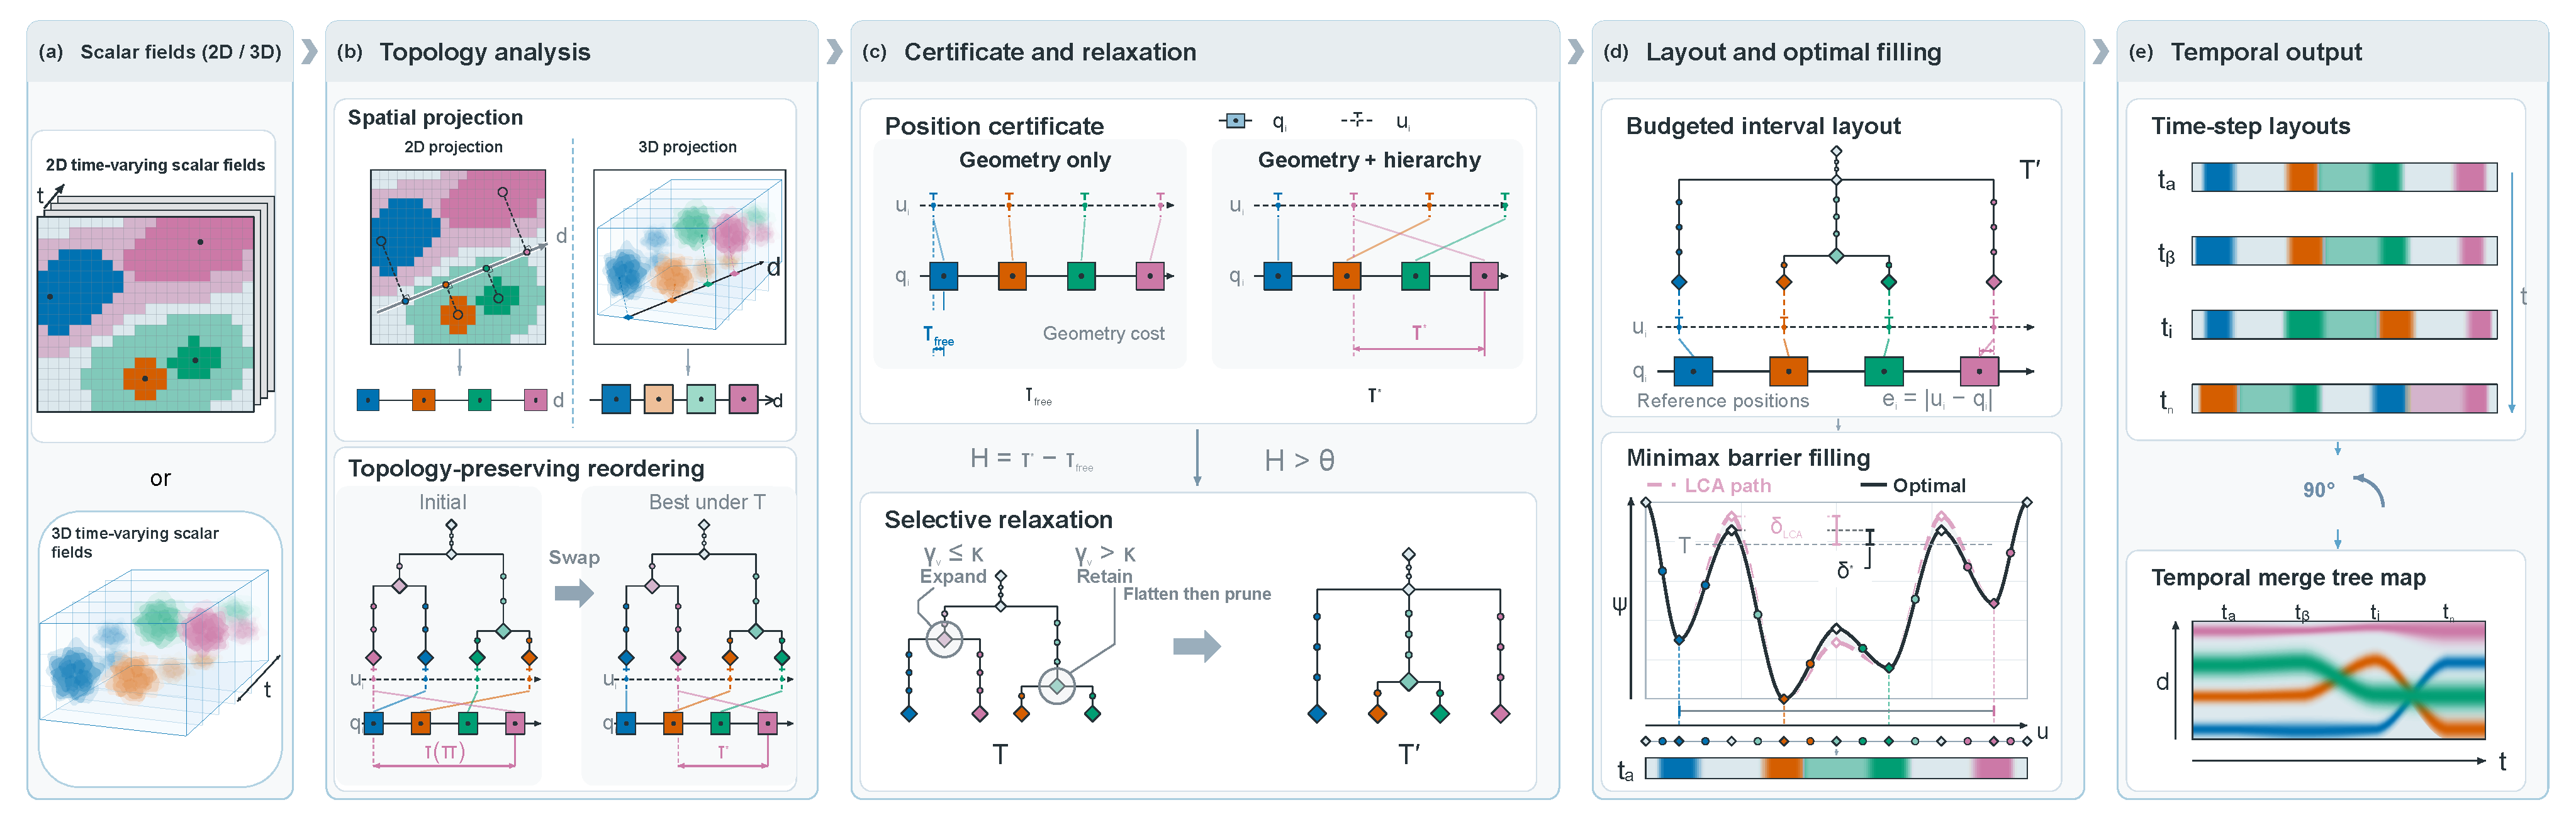
\includegraphics[width=\textwidth]{figures/Fig3.pdf}
\caption{RG-MTM's five stages (a)--(e), using the supplied four-feature schematic. Trees and a fixed projection define source merge targets and reference positions. Certificates diagnose hierarchy-dependent displacement; selective relaxation expands the ordering tree. Budgeted intervals and minimax filling construct profiles, stacked through time. The four branch identities retain blue, orange, green, and purple across stages; actual maps encode scalar values. Flatten-then-prune restoration is used in the planar protocol. $\kappa$ controls eligibility; output barriers determine measured cost.}
\label{fig:pipeline}
\end{figure*}

Figure~\ref{fig:pipeline} follows the data from scalar-field input through topology and projection, certificate-driven hierarchy choice, interval layout with optimal filling, and temporal assembly. The construction uses the source tree for scalar targets throughout; the ordering tree controls the permutations available to the layout.
Algorithm~\ref{alg:rgmtm} collects the construction and its hierarchy-selection and barrier routines in one procedure. Its inputs are augmented trees and tracked features from the extraction stage; its output records both the map and the achieved errors.
\begin{algorithm}[t]
\caption{Reference-guided temporal merge tree maps.}\label{alg:rgmtm}
\small
\algrenewcommand{\algorithmicrequire}{\textbf{Data:}}
\algrenewcommand{\algorithmicensure}{\textbf{Result:}}
\algrenewcommand{\algorithmicfunction}{\textbf{Function}}
\begin{algorithmic}
\Require Augmented trees $T_t$, extrema, supports, matches, domain $\Omega$; mode P/R and parameters $\theta,\kappa,\beta,\mathcal G$
\Ensure Temporal map $\mathcal V$; position bounds, anchor residuals, and measured merge errors
\Function{BuildMap}{$\{T_t\},\mathrm{matches},\mathrm{mode}$}
 \State $(d,q,[a,a+L])\gets\Call{SharedReference}{\mathrm{extrema},\mathrm{matches},\Omega}$
 \For{each time step $t$}
  \State Set support widths and check packing on $[a,a+L]$
  \State $(\mathcal D_t,\underline H_t)\gets\Call{Diagnose}{T_t,q_t,\mathcal G_t}$
  \State $T'_t\gets\Call{ChooseTree}{T_t,\underline H_t,\mathrm{mode}}$
  \State $\overline\tau'_t\gets$ feasible certificate upper bound for $T'_t$
  \State $B_t\gets\overline\tau'_t+\beta$
  \State $\mathcal C_t\gets$ budget-feasible legal orders of $T'_t$: enumerate for small trees; at most four candidates for large trees
  \State $(\pi,z,u)\gets$ best feasible layout from candidate QPs, using the preceding frame's matched layout
  \State $(v_t,\alpha)\gets\Call{RasterizeAndFill}{T_t,\pi,z,u}$
  \If{$T'_t\ne T_t$}
   \State $(b,\delta^*)\gets\Call{OptimalBarriers}{\pi,T_t}$
   \State Correct $v_t$ to barriers $b$ with strict-extremum clearance; retain anchor values at $\alpha$
  \EndIf
  \State Record $\mathcal D_t$, anchor residuals, and merge error measured from $v_t$ against $T_t$
 \EndFor
 \State \Return columns $[v_1\ \cdots\ v_K]$ with shared scalar colors
\EndFunction
\Statex
\Function{ChooseTree}{$T,\underline H,\mathrm{mode}$}
 \If{mode P or $\underline H\le\theta$} \State \Return $T$ \EndIf
 \State $W\gets$ non-root branching nodes with $\gamma_v\le\kappa$
 \State $T'\gets\mathrm{flat}(T,W)$
 \If{planar protocol}
  \State $b_0\gets$ grid-certificate score of $T'$
  \State Restore constraints in $T'$ by decreasing $\gamma_v$ while its score stays within half a pixel of $b_0$
 \EndIf
 \State \Return $T'$
\EndFunction
\Statex
\Function{OptimalBarriers}{$\pi,T$}
 \If{fewer than two leaves} \State \Return no barriers, $0$ \EndIf
 \State Renumber leaves by $\pi$; obtain original LCA levels $M_{ij}$
 \State $C_k\gets\min_{i\le k<j}M_{ij}$ for each inter-anchor gap $k$
 \State $\delta\gets\max(0,\max_k[\max(f_k,f_{k+1})-C_k])$
 \For{each leaf pair $i<j$}
  \State $\delta\gets\max\bigl(\delta,[M_{ij}-\max_{i\le k<j}C_k]/2\bigr)$
 \EndFor
 \State \Return $C+\delta$, $\delta$
\EndFunction
\end{algorithmic}
\end{algorithm}


\subsection{Shared Reference and Diagnosis}\label{sec:reference}
\textsc{SharedReference} derives one sequence-wide direction from consecutive-frame matches. It accumulates the outer products of matched extremum displacements, takes the leading unit eigenvector, and orients its sign toward the total displacement. Projecting retained extrema and domain corners then fixes the reference coordinates and canvas for all columns. A supplied direction supports a selected geographic axis. Feature widths use area or volume with the same conversion factor over the sequence.

\textsc{Diagnose} assigns each frame position costs, hierarchy cost, and conflict triples. Exact small-tree evaluation returns $\tau^*(T_t)$, $\tau_{\free,t}$, and $H_t$; a bounded large-tree evaluation retains lower and upper endpoints for both position costs. Its nonnegative hierarchy lower bound is $\underline H_t=\max(0,\underline\tau^*(T_t)-\overline\tau_{\free,t})$, which coincides with $H_t$ when both costs are exact. The gate uses this lower bound; layout uses a feasible positional upper bound. Conflict triples identify which feature relations exclude the desired order.

\subsection{Preserving and Relaxed Ordering Trees}\label{sec:relaxation}
RG-MTM-P sets $T'_t=T_t$. RG-MTM-R activates when $\underline H_t>\theta$ and marks non-root branching nodes with $\gamma_v\le\kappa$ as eligible. Flattening these nodes joins their child blocks to their parent and permits additional interleavings while retaining all leaves. The original merge targets remain in $T_t$.

For the two-dimensional suite, restoration removes unnecessary flattenings. Compute the grid-certificate score $b_0$ after flattening every eligible node. Visit nodes in decreasing merge-gap order and restore a constraint whenever its score stays within half a pixel of the fixed $b_0$. The resulting tree retains the original constraints that fit the initial relaxed position score. Volumetric construction retains the eligible flattenings and uses the large-tree search described below.

Shared settings use $c|\Omega|=L/2$, $\rho=0.5$, $g=L/240$, $\beta=L/120$, and $\theta=0.02L$, with domain area or volume for $|\Omega|$. The main planar temporal setting is $\kappa=0.2\Delta_F$, where $\Delta_F$ is the fixed processed scalar range. We abbreviate eligibility fractions 2\%, 20\%, and 100\% as R2, R20, and R100. This threshold selects eligible parent gaps; it does not cap the rendered merge-level error. \textsc{OptimalBarriers} computes the selected order's scalar cost. The static and volumetric protocols retain their declared simplification, candidate-search, and relaxation settings (Supplement S6 and S9).

\subsection{Budgeted Interval Layout}
The position budget $B_t=\overline\tau'_t+\beta$ uses a feasible positional upper bound and reserves allowance for geometric and temporal objectives; exact diagnosis gives $\overline\tau'_t=\tau^*(T'_t)$. For each budget-feasible legal order, a convex quadratic layout combines four mean squared residuals: anchor-reference offsets (weight 4), ordered anchor distances versus support-centroid distances (1), matched projected-motion residuals (0.5), and anchor eccentricities (0.1). The motion residual subtracts the projected source displacement from the matched anchor displacement. The interval geometry and $|u_i-q_i|\le B_t$ constrain the coordinates; the smallest evaluated objective selects the layout sequentially through time.

Small-tree construction enumerates legal orders and evaluates their continuous position costs. Large-tree construction propagates continuous earliest-finish Pareto functions through low-degree nodes; higher-degree cases use workload bounds or a time-limited mixed-integer program. Each result retains a lower bound, a feasible upper bound, and a witnessing order. Layout uses the upper bound plus $\beta$ and evaluates up to four legal candidates assembled from the certificate, reference-preferred, temporal-preferred, and TMTM orders. Fixed-order convex QPs record feasibility and first-order objective gaps. Figure~\ref{fig:pipeline} summarizes the construction; Supplement S1 details the planar construction and S6 the volumetric solver protocol.

\paragraph{Guarantees and selection.}
For a fixed order, the position cost and non-strict scalar cost are exact quantities of the display model. Exact small-tree enumeration also resolves the attainable frontier. The constructed map instead selects a secondary objective within a feasible position budget; a finite large-tree candidate set does not establish global optimality over all legal orders. Certificate intervals disclose unresolved position costs, and measured anchor and barrier errors describe the actual output. This distinction applies equally to preserving and relaxed modes.

\subsection{Scalar Filling and Temporal Assembly}\label{sec:domain_filling}
\begin{figure}[t]
\centering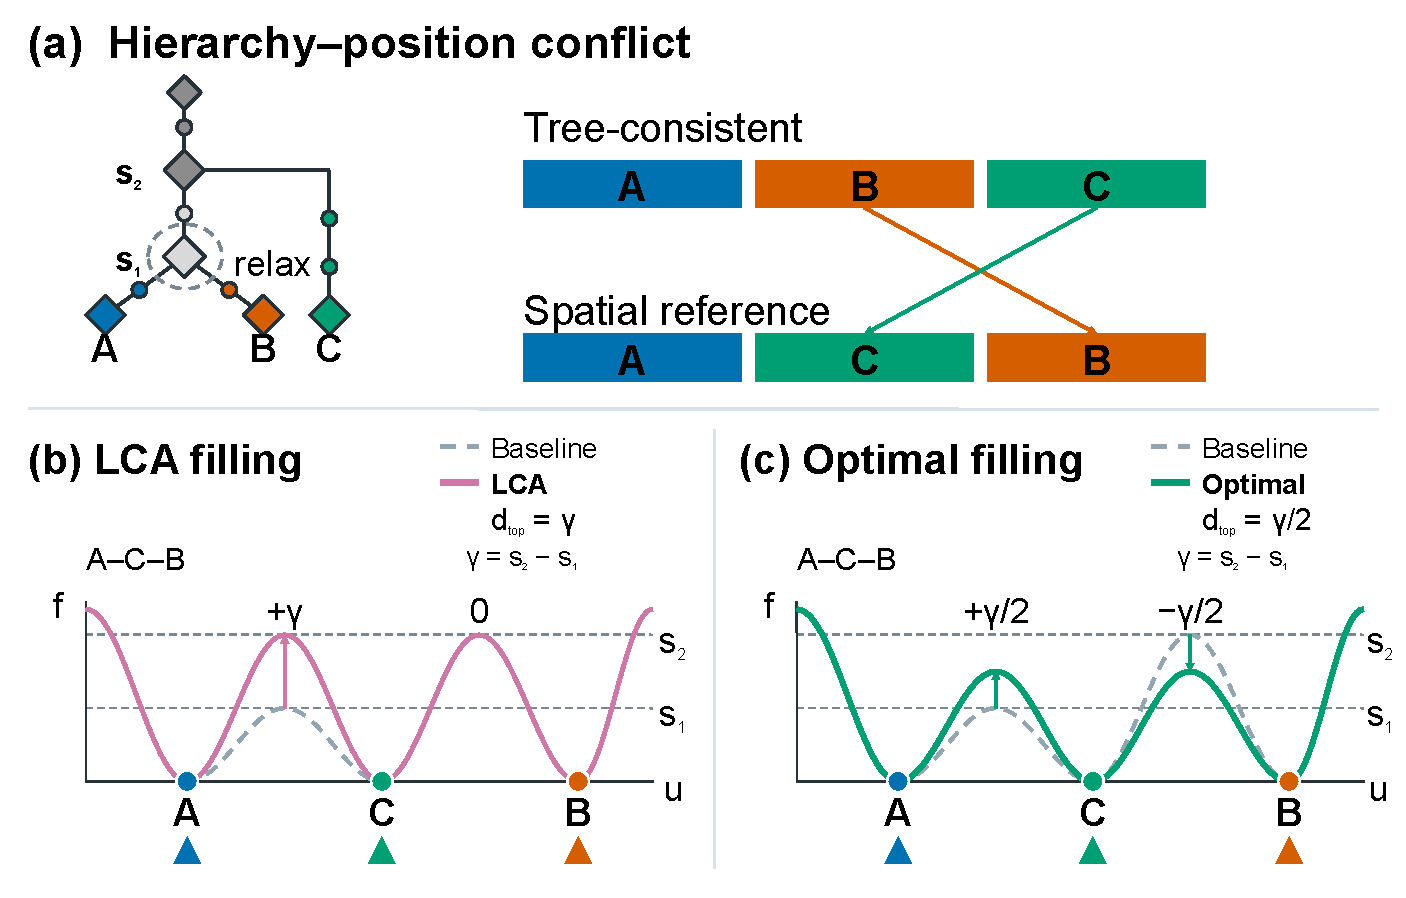
\includegraphics[width=\linewidth]{figures/Fig4.pdf}
\caption{Hierarchy--position conflict and scalar filling for three equal-valued minima. (a) The source tree groups $A,B$, excluding reference order $A,C,B$. Identity colours match the other schematics: $A$ blue, $B$ orange, and $C$ green. (b,c) Both fillings use the same relaxed anchors in order $A,C,B$, with identical reference triangles. Original-LCA filling (purple) sets both barriers to $s_2$, incurring $d_{\rm top}=\gamma=s_2-s_1$. Optimal filling (green) places both at $(s_1+s_2)/2$, attaining $\gamma/2$ when fixed leaf values lie below this level. The dashed grey baseline retains the hierarchy and its anchor displacement. Curves are schematic.}
\label{fig:filling}
\end{figure}

Scalar filling reuses ST-MTM's leaf-arc and hierarchical-path construction~\cite{STMTM:2026}. True extremum values occupy the anchors; resampled arc values alternate around them. Inter-anchor gaps follow original-tree LCA paths, allocating sibling, direct--deep, and deep--deep cases according to their arc lengths. Root paths fill the borders; Supplement S2 details each case.
\textsc{RasterizeAndFill} denotes this initial rendering on the shared canvas. \textsc{OptimalBarriers} uses join-tree values; split-tree values are negated before correction and transformed back afterwards. Its returned $\delta^*$ is the analytical fixed-order cost; measured raster error is recorded after clearance and filling.

RG-MTM-P retains the original merge barriers. For a relaxed order, call \textsc{OptimalBarriers}, clip each inter-anchor segment at its returned barrier, and raise its peak to that level when needed. Endpoint extrema retain their values. Figure~\ref{fig:filling} separates the order change from its scalar correction. The source tree $((A,B),C)$ excludes reference order $A,C,B$. For that relaxed order, original-LCA filling sets both inter-anchor barriers to $s_2$, changing the $A/B$ merge by $\gamma=s_2-s_1$. Optimal filling balances the three pairwise discrepancies at $\gamma/2$ by placing both barriers at $(s_1+s_2)/2$, provided the fixed leaf values lie below that midpoint. The dashed grey preserving profile shows the anchor displacement removed by the new order; the purple and green curves isolate filling quality at the same relaxed anchors.

The renderer maps the fixed canvas to the same raster coordinates at every time step and stacks columns chronologically. Shared colours encode scalar values; matched extrema form temporal tracks. Each frame records its position certificate, achieved anchor residuals, and actual merge-level error measured from the filled column. Nearest-pixel anchor rounding contributes at most $L/[2(N-1)]$ for raster length $N$, with capacity checked before filling.

\section{Quantitative Evaluation}\label{sec:eval}
We first test the common-model operating regimes and descriptive similarity to native methods (RQ1), then continuous budget feasibility and inverse queries (RQ2). Retained shared-input comparisons and source-linked cases examine practical consequences (RQ3). New common-QP measurements, frontier witnesses and earlier P/R measurements retain separate result identities and guarantees.

\subsection{Data Sets, Protocol, and Measures}
Table~\ref{tab:datasets_main} lists all nine evaluated inputs, their scalar fields, spatial dimensions, grids, sample counts, extracted leaves, and tree types. The five planar temporal sequences contain 614 frames: Storms (118 half-day pressure fields), Wildfires (30 two-day fire-radiative-power aggregates), OLR (60 daily fields), PM2.5 (366 fields covering all of 2000), and synthetic Ring (40 frames)~\cite{Hersbach:2020:ERA5,Franke:2021:1DP,NOAA:OLR,Dong:2026:PM25,Koepp:2023:TMTM}. The separate 744-hour Storms overview and 64-frame mirror control do not enter the 614-frame small-tree statistics.

The remaining planar inputs are the original author $64\times64$ static Nucleon slice and 21 static sections of an explicitly reconstructed Benzene point-charge potential~\cite{Koepp:2023:TMTM,Jorgensen:2013:BOSS,Inviwo:BenzeneGeometry}. Tangaroa subsequently supplies 201 original-grid three-dimensional velocity-magnitude fields, and Cylinder supplies 102 three-dimensional $Q$ fields derived from public velocity volumes~\cite{Popinet:2004:Tangaroa,Camarri:2005:Cylinder,Weinkauf:SquareCylinder}. Section index is not physical time. All nine inputs appear together in Table~\ref{tab:tradeoff}; input dimensions and independent populations remain explicit. The seven temporal inputs comprise 917 fields, without forming a pooled accuracy score.

All methods share each input's processed fields, extrema, supports, and overlap matches. Retained temporal-construction comparisons use shared-input TMTM and ST-MTM reimplementations, RG-MTM-P, and RG-MTM-R at $\kappa/\Delta_F=0.20$. ST-MTM uses uniform distance weights, $r=0.95$, and temporal weight $0.5$ (Ring: $1.5$). The previously omitted Nucleon, Benzene, Tangaroa and Cylinder comparisons have now been computed on all 325 retained inputs with these fixed generic settings and 32768-row profiles. Nucleon uses base mode; Benzene propagates across spatial sections without assigning physical time. For the volumetric extension, the same equations use three-dimensional centroid distances. A deterministic equal-level binary refinement handles multifurcations while preserving all source leaf supports and labelled merge levels; it restricts the admissible leaf orders and is an implementation assumption. Supplement S3 records the equations, width units, solver checks and complete results; this is a shared-input extension rather than reproduction of unpublished original presets. The RG modes share geometry and secondary objectives. An independent 148-frame Storms/Wildfires audit matches 486 TMTM branch decisions and 1118 interval/anchor records to the official C++ core, and checks ST-MTM objectives, constraints, and rendered topology (Supplement S7). Supplemental controls comprise native Hilbert/Morton traversals, packed reference sorting, fixed axes, and exact reference projection. Supplements S2, S6, and S9 retain all acquisition, smoothing, cropping, boundary, simplification, and solver settings.

\begin{table*}[t]
\caption{All nine inputs evaluated with the shared error definitions. Source dimension describes the input, not the two-dimensional map output.}\label{tab:datasets_main}
\centering\footnotesize\setlength{\tabcolsep}{4pt}
\begin{tabular}{lllrlll}\toprule
Data & Input & Scalar field & Processed grid & Samples & Leaves & Tree\\\midrule
Storms & 2-D & Mean sea-level pressure & $49\times49$ & 118 frames & 1--8 & Join\\
Wildfires & 2-D & $\log(1+\mathrm{FRP})$ & $64\times64$ & 30 frames & 6--11 & Split\\
OLR & 2-D & Outgoing longwave radiation & $49\times49$ & 60 frames & 2--8 & Join\\
PM$_{2.5}$ & 2-D & PM$_{2.5}$ concentration & $49\times49$ & 366 frames & 1--7 & Split\\
Ring & 2-D & Synthetic ring intensity & $14\times14$ & 40 frames & 1--7 & Split\\
Tangaroa & 3-D & Velocity magnitude & $300\times180\times120$ & 201 frames & 18--93 & Join\\
Cylinder & 3-D & Q criterion & $135\times64\times48$ & 102 frames & 4--75 & Split\\
Nucleon & 2-D & Nucleon scalar & $64\times64$ & 1 slice & 13 & Split\\
Benzene & 2-D & Reconstructed electrostatic potential & $61\times61$ & 21 sections & 5--10 & Join\\
\bottomrule\end{tabular}
\par\smallskip{\footnotesize\raggedright Storms, Wildfires, OLR and PM$_{2.5}$ are observed fields; Ring is synthetic. Tangaroa and Cylinder are volumetric simulations. Cylinder Q is computed on the original $192\times64\times48$ velocity grid before the $135\times64\times48$ crop. Nucleon is one author-provided static planar slice; Benzene is a reconstructed point-charge potential evaluated on 21 static sections. Seven temporal sequences contain 917 frames; static sections and the independent mirror control are separate populations.\par}
\end{table*}


\paragraph{Reference order and actual displacement.}
Normalized Reference-Order Error (NROE) evaluates the displayed anchor order $\pi_t$ independently of native scales and widths:
\begin{equation}
\begin{aligned}
 \mathrm{NROE}_t&=\frac{\max\{0,\max_{r<s}(q_{\pi_r}^t-q_{\pi_s}^t)\}}{2L},\\
 \mathrm{NROE}&=\operatorname{mean}_t\mathrm{NROE}_t .
\end{aligned}\label{eq:order_metric}
\end{equation}
It is the smallest maximum displacement after monotone calibration, with stable tie-breaking for coincident anchors; single-leaf frames have zero order error. Actual RG coordinates use $E_{\rm pool}=\sum_{t,i}|u_i^t-q_i^t|/(L\sum_t n_t)$ and $E_\infty=\max_{t,i}|u_i^t-q_i^t|/L$, computed from continuous layouts. These separate order compatibility from achieved position. The same continuous definitions apply to all nine inputs, including the volumetric and static cases; they do not substitute the older rendered, frame-averaged MAE.

\paragraph{Merge levels.}
Normalized Merge-Level Error is $D_t=d_{\rm top}(\psi_t,T_t)/\Delta_F$, using a fixed processed scalar range for the sequence. NMLE$_{\rm mean}$ averages framewise worst-pair errors; NMLE$_{\rm max}$ gives the worst frame. Values in Table~\ref{tab:tradeoff} are measured from filled-raster barriers. The analytical $\delta^*$ supplies the corresponding fixed-order prediction. This metric evaluates merge thresholds for corresponding leaves; it does not measure all changes to the scalar distribution or thresholded spatial regions.

\paragraph{Motion and geometry.}
A tracked pair supplies a clear approach/separation event when its two- or three-dimensional source-space Euclidean distance changes by more than 2\% of domain diagonal across two steps. The displayed decision uses anchor-distance change and a 2\% threshold of the method's sequence-wide occupied range, except Cylinder, whose retained protocol uses 2\% of the fixed full canvas for every method. This threshold convention is also used for its new ST-MTM run. Motion error ME counts reversals plus misses among shared $N_{\rm clear}$ events. Four-step circular temporal blocks give paired bootstrap intervals. Support-centroid scale-normalized stress (SNS), trustworthiness (TW), and full-canvas temporal displacement (TD) quantify additional geometric properties; their definitions and complete results are in Supplement S3. Motion counts are geometric diagnostics of overlap-linked extrema. Small event populations and static inputs are reported explicitly, and no aggregate accuracy is inferred from averaging datasets with different event counts.

\begin{table*}[t]
\caption{Complete shared-input evaluation, grouped by method. All 2-D inputs precede the 3-D volumes in every panel.}\label{tab:tradeoff}
\centering\footnotesize\setlength{\tabcolsep}{2pt}
\textit{(a) Reference order, motion and merge-level cost}\par\smallskip
\begin{tabular*}{\textwidth}{@{\extracolsep{\fill}}lrrrrrrrrrrr@{}}\noalign{\hrule height .8pt width \textwidth\vskip 2.5pt}
 & & \multicolumn{2}{c}{TMTM} & \multicolumn{2}{c}{ST-MTM} & \multicolumn{2}{c}{RG-MTM-P (ours)} & \multicolumn{4}{c}{RG-MTM-R (ours)}\\
\cmidrule(lr){3-4}\cmidrule(lr){5-6}\cmidrule(lr){7-8}\cmidrule(lr){9-12}
Data & $N_{\rm clear}$ & NROE$\downarrow$ & ME$\downarrow$ & NROE$\downarrow$ & ME$\downarrow$ & NROE$\downarrow$ & ME$\downarrow$ & NROE$\downarrow$ & ME$\downarrow$ & NMLE$_{\rm mean}\downarrow$ & NMLE$_{\rm max}\downarrow$\\\midrule
Storms & 104 & 19.23 & 0.471 & 16.28 & 0.413 & 3.77 & 0.231 & 1.16 & 0.183 & 1.47 & 26.07\\
Wildfires & 112 & 29.30 & 0.393 & 24.02 & 0.357 & 5.83 & 0.321 & 0.34 & 0.312 & 3.96 & 19.56\\
OLR & 56 & 19.31 & 0.446 & 17.21 & 0.214 & 0.89 & 0.054 & 0.00 & 0.054 & 1.10 & 33.56\\
PM2.5 & 95 & 12.87 & 0.453 & 11.60 & 0.516 & 0.98 & 0.442 & 0.01 & 0.495 & 0.18 & 4.67\\
Ring & 124 & 7.18 & 0.645 & 10.39 & 0.347 & 2.66 & 0.315 & 0.13 & 0.129 & 2.73 & 12.35\\
Nucleon & -- & 11.9048 & -- & 11.9048 & -- & 2.3810 & -- & 2.3810 & -- & 0.0000 & 0.0000\\
Benzene & -- & 50.0000 & -- & 50.0000 & -- & 4.2063 & -- & 0.0000 & -- & 0.0025 & 0.0080\\
Tangaroa & 6755 & 20.09 & 0.975 & 21.34 & 0.700 & 9.61 & 0.547 & 0.02 & 0.305 & 14.44 & 31.02\\
Cylinder & 3196 & 26.62 & 0.670 & 17.77 & 0.460 & 12.26 & 0.373 & 0.08 & 0.189 & 2.81 & 14.28\\
\bottomrule\end{tabular*}
\par\medskip
\textit{(b) Standard geometry and temporal stability}\par\smallskip
\begin{tabular*}{\textwidth}{@{\extracolsep{\fill}}lrrrrrrrrrrrr@{}}\noalign{\hrule height .8pt width \textwidth\vskip 2.5pt}
 & \multicolumn{3}{c}{TMTM} & \multicolumn{3}{c}{ST-MTM} & \multicolumn{3}{c}{RG-MTM-P (ours)} & \multicolumn{3}{c}{RG-MTM-R (ours)}\\
\cmidrule(lr){2-4}\cmidrule(lr){5-7}\cmidrule(lr){8-10}\cmidrule(lr){11-13}
Data & SNS$\downarrow$ & TW$_1\uparrow$ & TD$\downarrow$ & SNS$\downarrow$ & TW$_1\uparrow$ & TD$\downarrow$ & SNS$\downarrow$ & TW$_1\uparrow$ & TD$\downarrow$ & SNS$\downarrow$ & TW$_1\uparrow$ & TD$\downarrow$\\\midrule
Storms & 0.0799 & 0.8243 & 10.1108 & 0.0297 & 0.9653 & 7.1607 & 0.1186 & 0.7771 & 27.3609 & 0.1097 & 0.7554 & 23.8891\\
Wildfires & 0.2210 & 0.8170 & 11.2034 & 0.0786 & 0.9195 & 7.9585 & 0.0831 & 0.8793 & 8.0342 & 0.0579 & 0.8725 & 3.2487\\
OLR & 0.1419 & 0.8135 & 8.7479 & 0.0062 & 0.9751 & 2.3304 & 0.0121 & 0.9587 & 8.9011 & 0.0093 & 0.9634 & 8.5023\\
PM2.5 & 0.0509 & 0.7596 & 38.7546 & 0.0256 & 0.9223 & 7.7763 & 0.0640 & 0.7492 & 76.3170 & 0.0524 & 0.7291 & 68.7114\\
Ring & 0.1706 & 0.7067 & 1.3436 & 0.0803 & 0.9172 & 2.3641 & 0.1637 & 0.7087 & 3.5977 & 0.1423 & 0.7149 & 2.3512\\
Nucleon & 0.3122 & 0.9161 & -- & 0.0506 & 0.9860 & -- & 0.1325 & 0.8951 & -- & 0.1325 & 0.8951 & --\\
Benzene & 0.1750 & 0.6264 & -- & 0.1284 & 0.6254 & -- & 0.1588 & 0.4972 & -- & 0.1570 & 0.5258 & --\\
Tangaroa & 0.5255 & 0.6701 & 64.8553 & 0.1655 & 0.8137 & 138.5519 & 0.3571 & 0.7271 & 158.2670 & 0.3353 & 0.7458 & 39.7093\\
Cylinder & 0.2956 & 0.8017 & 85.0339 & 0.1346 & 0.8989 & 43.1663 & 0.1393 & 0.7838 & 72.3427 & 0.0399 & 0.8912 & 29.1130\\
\bottomrule\end{tabular*}
\par\medskip
\textit{(c) Continuous reference displacement and static-section coherence}\par\smallskip
\begin{tabular*}{\textwidth}{@{\extracolsep{\fill}}lrrrrrrrr@{}}\noalign{\hrule height .8pt width \textwidth\vskip 2.5pt}
 & TMTM & ST-MTM & \multicolumn{3}{c}{RG-MTM-P (ours)} & \multicolumn{3}{c}{RG-MTM-R (ours)}\\
\cmidrule(lr){2-2}\cmidrule(lr){3-3}\cmidrule(lr){4-6}\cmidrule(lr){7-9}
Data & SD$\downarrow$ & SD$\downarrow$ & $E_{\rm pool}\downarrow$ & $E_\infty\downarrow$ & SD$\downarrow$ & $E_{\rm pool}\downarrow$ & $E_\infty\downarrow$ & SD$\downarrow$\\\midrule
Storms & -- & -- & 4.13 & 26.19 & -- & 2.14 & 18.46 & --\\
Wildfires & -- & -- & 3.18 & 20.48 & -- & 0.80 & 6.64 & --\\
OLR & -- & -- & 1.00 & 17.14 & -- & 0.57 & 1.69 & --\\
PM2.5 & -- & -- & 1.87 & 20.26 & -- & 0.76 & 5.86 & --\\
Ring & -- & -- & 2.43 & 11.90 & -- & 0.71 & 2.52 & --\\
Nucleon & -- & -- & 1.92 & 3.43 & -- & 1.92 & 3.43 & --\\
Benzene & 4.1118 & 1.9658 & 1.60 & 15.39 & 2.4060 & 0.52 & 1.75 & 0.9601\\
Tangaroa & -- & -- & 5.01 & 16.86 & -- & 1.18 & 8.02 & --\\
Cylinder & -- & -- & 5.40 & 32.08 & -- & 0.55 & 5.27 & --\\
\bottomrule\end{tabular*}
\par\smallskip{\footnotesize\raggedright NROE and continuous $E$ are percentages of reference extent; NMLE is a percentage of the fixed processed scalar range. ME is the error fraction over the shared $N_{\rm clear}$ events (lag 2; 2\% source-distance threshold). Cylinder retains its 2\%-of-full-canvas display threshold; other temporal inputs use the method-specific occupied range. SNS uses scale-fitted squared centroid-distance residuals; TW uses $k=1$ on valid frames. TD sums matched displacements in full-canvas units. SD is the separately named adjacent-section displacement, available only for Benzene (170 spatial matches). -- denotes an inapplicable metric; native axes have no direct-reference $E$ without calibration. TMTM, ST-MTM and P have zero measured NMLE. R uses $\kappa=0.2\Delta_F$, an eligibility threshold rather than an achieved-error cap. Protocols and eligible counts are in Supplement S3.\par}
\end{table*}


\subsection{Established Geometry and Stability Metrics on 2-D Inputs}
We additionally evaluate the criteria used by ST-MTM~\cite{STMTM:2026}: scale-normalized stress (SNS), trustworthiness (TW), and temporal displacement (TD). SNS minimizes squared centroid-distance residuals over one positive scale per frame, without a square root; lower is better. TW penalizes introduced neighbours by their original-space rank; higher is better. We fix $k=1$ across all inputs and average only frames satisfying $k<n/2$. TD is the sum of matched-anchor absolute changes after one fixed full-canvas mapping per sequence, not a frame average or occupied-range normalization. Supplement S3 lists all eligible frame counts and exact formulas.

The completed planar comparison distinguishes alignment from relative geometry. ST-MTM retains better SNS, TW and TD than R20 on Storms, OLR and annual PM2.5. R20 has lower SNS on Wildfires and lower TD on Wildfires and Ring, while its TW remains lower on all five temporal inputs. These complementary outcomes support a controlled reference--geometry trade-off, rather than universal superiority.

Both static planar inputs now have all four methods' SNS and TW. Nucleon ST-MTM attains SNS 0.0506 and TW 0.9860; P/R attain 0.1325 and 0.8951 despite their lower reference-order error. On Benzene, ST-MTM SNS is 0.1284 versus R20's 0.1570, whereas R20 has smaller summed adjacent-section displacement (0.9601 versus 1.9657 canvas widths over the same 170 matches). Temporal ME and TD are undefined for both static inputs. Section displacement is a separate spatial-coherence measurement, not a zero temporal error.

\subsection{Operating Regimes of One Model (RQ1)}
We recompute topology--time, topology--geometry, and reference-guided layouts at topology allowances 0, 2\% and 10\% on the same five planar sequences. This produces 3070 layouts from 614 frames. All five settings share each frame's candidate pool, widths, canvas, scalar range, source-value renderer and convex QP implementation. They differ only in the controls in Table~\ref{tab:profiles}; the main regime comparison disables the reference cap ($B=\infty$). A separate Ring grid fixes the reference objective and evaluates all nine combinations of $\varepsilon\in\{0,0.02,0.1\}$ and $B\in\{\infty,0.1,0.05\}$.

The common-model search covers all permutations on 496 frames; the other 118 frames use recorded candidate pools. Across the five settings it evaluates 15141 admissible fixed-order QPs. These coverage counts describe the new QP experiment, not the independently exhaustive frontier experiment below. Selected continuous layouts satisfy their topology and position caps, and the largest normalized candidate-objective gap bound is 1.2e-06. Independent saved-witness checks reconstruct the objective, constraints and selected-order first-order gaps.

Geometry activation reduces the geometry residual relative to the topology--time setting on all five tested inputs. Reference activation greatly reduces absolute reference error, while changing the temporal target from stationary alignment to projected-motion following. These changes express distinct priorities rather than a universal quality ranking. The 2\% and 10\% scalar allowances further reduce pooled reference error on all five sequences in this run, but no monotonic improvement in every component or recomputed temporal history is claimed. Table~\ref{tab:unified_regimes} reports all component measures; Figures~\ref{fig:unified_regimes}--\ref{fig:unified_budget_grid} show the resulting maps.

The shared-input native TMTM and ST-MTM reimplementations are run independently on Ring and Storms. Descriptive similarity uses labelled-pair order agreement and anchor RMSE after one sequence-wide affine gauge fit, including reflection. The fit does not modify the underlying layouts or any reference-error metric. Table~\ref{tab:unified_similarity} reports the results. The topology--time regime is an anchor-alignment surrogate for TMTM, and the topology--geometry regime uses common interval rules instead of ST-MTM's native allocation. In particular, low Storms agreement with native ST-MTM exposes a substantive difference; common design priorities do not imply universally close coordinates. Independent baseline audits retain their separate evidence role in Supplement S7.

The unit tests also isolate an important control: a zero reference weight can still leave a reference-dependent hard position cap. Explicitly disabling that cap recovers geometry-only behavior on a two-feature example, and the canonical null-space rule resolves free newborn coordinates without changing the primary objective. These checks support the interpretation of the parameter regimes rather than native-algorithm equivalence.

\begin{table*}[t]
\caption{New common-model results on all 614 planar frames, with five settings each (3070 layouts). All numbers are percentages: pooled absolute reference error (R-MAE), root mean framewise geometry/temporal squared residual (G-RMS, stationary S-RMS and projected-motion M-RMS), and worst continuous labelled merge error (Top-max). Geometry and temporal quantities use the common fixed canvas, not native-baseline scales. Empty pair/match terms contribute zero. First-frame temporal terms are zero. Different components express competing priorities; lower reference error need not improve every score.}\label{tab:unified_regimes}
\centering\small
\begin{tabular}{llrrrrr}\toprule
Input & Regime & R-MAE & G-RMS & S-RMS & M-RMS & Top-max\\\midrule
Ring & Topology--time & 27.37 & 18.15 & 0.28 & 2.64 & 0.00 \\
Ring & Topology--geometry & 29.75 & 5.88 & 2.66 & 3.67 & 0.00 \\
Ring & Reference, 0\% & 2.57 & 8.58 & 3.97 & 3.42 & 0.00 \\
Ring & Reference, 2\% & 2.28 & 8.41 & 3.33 & 2.66 & 1.49 \\
Ring & Reference, 10\% & 1.17 & 8.15 & 2.65 & 1.20 & 9.40 \\
Storms & Topology--time & 25.31 & 47.41 & 0.38 & 18.65 & 0.00 \\
Storms & Topology--geometry & 33.56 & 11.73 & 8.86 & 19.46 & 0.00 \\
Storms & Reference, 0\% & 6.09 & 20.68 & 20.67 & 9.50 & 0.00 \\
Storms & Reference, 2\% & 5.78 & 20.61 & 20.67 & 8.51 & 1.31 \\
Storms & Reference, 10\% & 5.06 & 19.91 & 20.04 & 6.82 & 8.51 \\
Wildfires & Topology--time & 16.67 & 29.88 & 1.02 & 2.83 & 0.00 \\
Wildfires & Topology--geometry & 13.94 & 8.62 & 7.05 & 7.07 & 0.00 \\
Wildfires & Reference, 0\% & 3.19 & 10.03 & 6.89 & 6.13 & 0.00 \\
Wildfires & Reference, 2\% & 2.72 & 9.65 & 6.26 & 5.29 & 1.85 \\
Wildfires & Reference, 10\% & 1.84 & 9.01 & 5.16 & 4.13 & 8.35 \\
OLR & Topology--time & 24.43 & 35.53 & 0.56 & 9.42 & 0.00 \\
OLR & Topology--geometry & 42.71 & 4.26 & 4.94 & 11.63 & 0.00 \\
OLR & Reference, 0\% & 1.31 & 4.93 & 9.14 & 2.45 & 0.00 \\
OLR & Reference, 2\% & 1.17 & 4.80 & 9.11 & 2.37 & 1.79 \\
OLR & Reference, 10\% & 1.04 & 4.52 & 9.06 & 2.28 & 5.15 \\
PM$_{2.5}$ & Topology--time & 21.71 & 21.60 & 0.74 & 21.88 & 0.00 \\
PM$_{2.5}$ & Topology--geometry & 25.03 & 6.40 & 4.38 & 22.24 & 0.00 \\
PM$_{2.5}$ & Reference, 0\% & 3.05 & 10.60 & 22.07 & 5.44 & 0.00 \\
PM$_{2.5}$ & Reference, 2\% & 2.43 & 9.93 & 21.98 & 4.40 & 1.81 \\
PM$_{2.5}$ & Reference, 10\% & 2.15 & 9.61 & 21.80 & 3.54 & 4.67 \\
\bottomrule\end{tabular}\end{table*}

\begin{table}[t]
\caption{Descriptive similarity of inspired regimes to their native comparison methods. One sequence-wide least-squares affine transform, including reflection, aligns native anchors to the inspired anchors; no framewise fit is used. Agreement counts non-tied labelled feature pairs. RMSE is a percentage of the common inspired canvas. Values measure similarity, not algorithm recovery.}\label{tab:unified_similarity}
\centering\small
\begin{tabular}{llrrr}\toprule
Input & Native & Order (\%) & RMSE (\%) & Pairs\\\midrule
Ring & TMTM & 80.6 & 1.37 & 346 \\
Ring & ST-MTM & 77.2 & 9.69 & 346 \\
Storms & TMTM & 72.5 & 5.98 & 596 \\
Storms & ST-MTM & 51.7 & 34.24 & 596 \\
\bottomrule\end{tabular}\end{table}


\subsection{True Error Budgets and Inverse Queries (RQ2)}\label{sec:budget_experiments}
We newly evaluate nine normalized topology allowances $\{0,0.005,0.01,0.02,0.05,0.1,0.2,0.5,1\}$ on the unchanged five-sequence input population of 614 frames. Every frame uses the same fixed reference, canvas and absolute width convention across the sweep. All permutations are evaluated up to $8!=40320$ orders: 603 frames are exhaustive. The remaining 11 Wildfires frames use the fixed candidate set in Section~\ref{sec:hard_budget}; their values are feasible upper bounds, not certified global minima. No frames are excluded from the reported means.

The run constructs 5526 LP-anchor/barrier witnesses and evaluates 3684 inverse queries at six position caps. Every returned continuous witness meets its declared scalar allowance. No frame's selected position cost increases as $\varepsilon$ increases. The inverse query reports failure when no admissible order meets the requested position cap; on a candidate-only frame this means that no witness was found, rather than global infeasibility. Exhaustive frames supply the stronger interpretation.
\begin{table*}[t]
\caption{New hard-budget experiments on all 614 planar temporal frames. Position columns report the temporal mean of the framewise minimax absolute position error, in percent of the fixed reference extent. These are not NROE or the achieved secondary-QP errors in the retained tables. Wildfires includes 11 candidate-only upper bounds. The inverse column counts frames with a witnessed solution at a 2\% position cap and unrestricted scalar allowance; it is not the count attainable at a 2\% topology cap.}\label{tab:budget_results}
\centering\small
\begin{tabular}{lrrrrr}\toprule
Input & Exact/total & $\varepsilon=0$ & $\varepsilon=2\%$ & $\varepsilon=10\%$ & $E_t(2\%)$ feasible\\\midrule
Storms & 118/118 & 4.326 & 3.499 & 1.889 & 115/118 \\
Wildfires & 19/30 & 6.178 & 3.482 & 1.926 & 30/30 \\
OLR & 60/60 & 0.960 & 0.639 & 0.332 & 60/60 \\
PM$_{2.5}$ & 366/366 & 1.282 & 0.533 & 0.121 & 358/366 \\
Ring & 40/40 & 2.876 & 1.688 & 0.112 & 40/40 \\
\bottomrule\end{tabular}
\end{table*}


At a genuine 2\% topology cap, mean minimax position error changes from 4.326\% to 3.499\% on Storms, 6.178\% to 3.482\% on Wildfires, 0.960\% to 0.639\% on OLR, 1.282\% to 0.533\% on annual PM2.5, and 2.876\% to 1.688\% on Ring. These quantities are continuous per-frame minimax values, not NROE and not the achieved coordinates of the retained secondary-QP layouts. Figure~\ref{fig:budget_response} shows the budget response and illustrative Ring maps generated from the saved witnesses.

At a requested position cap of 2\% with unrestricted scalar allowance, the system finds witnesses in 115/118 Storms, 30/30 Wildfires, 60/60 OLR, 358/366 PM2.5 and 40/40 Ring frames. The three unsuccessful Storms and eight PM2.5 frames were exhaustively searched: their fixed widths and canvas prevent the target even after releasing topology. The inverse query returns a different minimum topology allowance for each feasible frame; these counts do not imply that a 2\% topology cap suffices. A sequence-wide feasibility claim uses the worst frame, whereas Table~\ref{tab:budget_results} reports temporal means.

\paragraph{Scope and controls.}
These experiments establish the continuous non-strict framewise budget behavior. They do not reuse the earlier motion scores as measurements of the new LP witnesses, establish a temporal-QP optimum, or certify a rounded raster under the same cap. The Ring illustrations have finite display resolution and are not used for the numerical guarantees. Existing P/R results below remain separate temporal-construction operating points; their parameter $\kappa$ is an eligibility threshold rather than $\varepsilon$.


\subsection{Retained Position Certificates and Scalar Correction}
\begin{figure*}[t]
\centering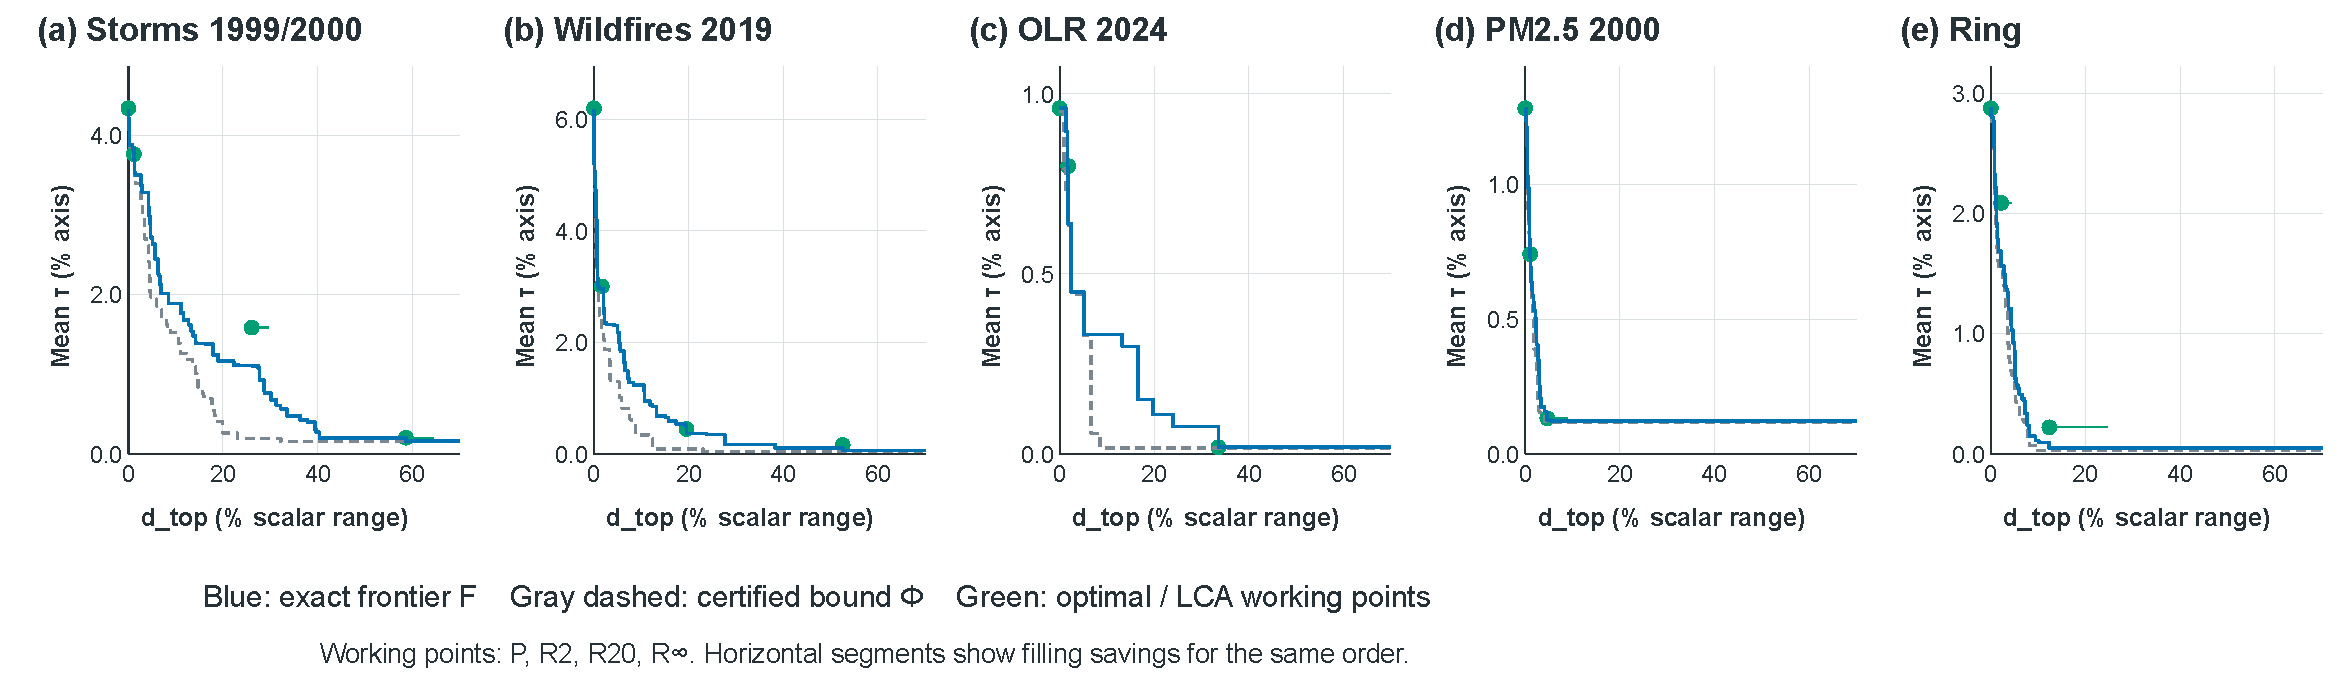
\includegraphics[width=\textwidth]{figures/Fig5.pdf}
\caption{Position--topology trade-offs for all five current planar temporal inputs, including complete-year PM2.5. Curves show temporal means of exact per-frame frontiers $F$ (blue) and certified lower bounds $\Phi$ (dashed) at a common scalar budget. Green points compare optimal (filled) and original-LCA (open) filling for identical selected orders at $\kappa/\Delta_F\in\{0,0.02,0.20,\infty\}$. Their horizontal coordinates are cross-frame maximum scalar costs; vertical coordinates are mean fixed-order position optima $\tau(\pi)$. Horizontal segments show scalar-filling savings for a fixed order. These common-budget curves differ from the per-frame 611/614 frontier-attainment check.}
\label{fig:diagnosis}
\end{figure*}

Hierarchy cost exceeds 2\% of reference extent in 40/118 Storms, 19/30 Wildfires, 7/60 OLR, 36/366 PM2.5, and 21/40 Ring frames. Hierarchy contributes more than packing in every sequence: respective mean costs are 4.17\%/0.16\% on Storms and 6.12\%/0.06\% on Wildfires; Supplement S3 retains all five pairs.

Independent LP and order-enumeration checks connect the position formulas to feasible layouts. Measured barriers agree with the optimal filling to within $1.2\times10^{-5}$ of the processed scalar range, including the strict-extremum clearance. TMTM, ST-MTM, and RG-MTM-P have zero measured labelled pairwise merge error across all suite frames. For the selected RG-MTM-R orders, fixed-order position optima reach the exact frontier within half a 1024-grid pixel in 611/614 frames. Figure~\ref{fig:diagnosis} shows all five current planar temporal sequences, including full-year PM2.5. The 611/614-frame check uses each frame's own measured scalar cost; the plotted mean curves instead use one common budget. Frontiers use one common budget; working points combine mean positional optima with maximum scalar costs. Table~\ref{tab:tradeoff} separately measures final anchors.

Holding the selected order fixed isolates scalar correction. Optimal barriers reduce mean Storms NMLE from 2.07\% for original-LCA filling to 1.47\%, and Ring from 5.46\% to 2.73\%. Packed reference sorting reaches zero Storms NROE with 6.18\% mean NMLE, compared with RG-MTM-R's 1.47\%. These controls separate the effects of reference ordering, hierarchy choice, and barrier construction.

\subsection{Retained Temporal Profiles: Reference, Geometry and Motion}
Within the five-sequence planar suite, RG-MTM-P lowers NROE relative to both baselines on every sequence while retaining the source merge levels (Table~\ref{tab:tradeoff}). Storms changes from ST-MTM's 16.28\% to 3.77\%, and Wildfires from 24.02\% to 5.83\%. This isolates the benefit of a reference-guided layout within the original hierarchy.

Relaxation improves NROE and pooled displacement on all five planar temporal sequences. Storms changes from 3.77\% to 1.16\% NROE, 4.13\% to 2.14\% pooled displacement, and 26.19\% to 18.46\% maximum displacement. Wildfires reaches 0.34\% NROE and 0.80\% pooled displacement. Table~\ref{tab:tradeoff} retain every sequence's order and coordinate measurements.

For the five planar temporal sequences, mean relaxed NMLE ranges from 0.18\% to 3.96\%, with maxima of 4.67\%--33.56\%. Storms incurs 1.47\% mean and 26.07\% maximum NMLE; Wildfires incurs 3.96\% and 19.56\%. These measured barriers quantify both sequence-wide and worst-frame costs against the source trees.

% Figure 1 shows RG-MTM-R20; the Storms four-method detail is in Supplement S8.

On Storms, motion-proxy errors decrease from ST-MTM's 43/104 to RG-MTM-R's 19/104 events. The paired difference is $-23.1$ percentage points, with a 95\% temporal-block interval of $[-33.6,-12.8]$. Ring decreases from 43/124 to 16/124. The complete table preserves each input's shared event counts and both RG modes. Tangaroa and Cylinder use three-dimensional spatial truth, whereas planar sequences use two-dimensional truth; static inputs have no temporal-motion score. Supplemental projected-motion scores use separate event populations.

On annual PM2.5, improved reference order does not yield improved spatial-motion classification: P makes 42/95 errors and R20 makes 47/95, compared with ST-MTM's 49/95. This full-year result supersedes the selected January example. Geometry remains a complementary criterion. On Wildfires, R reduces ST-MTM's SNS from 0.0786 to 0.0579 and TD from 7.9585 to 3.2487. Supplement S3 gives all geometric results, direction/persistence/extraction/eligibility controls, baseline settings, motion windows, and the separate large binary-tree benchmark.

\subsection{Absolute Reference and Hierarchical Ordering}\label{sec:reference_control}
\begin{figure*}[t]
\centering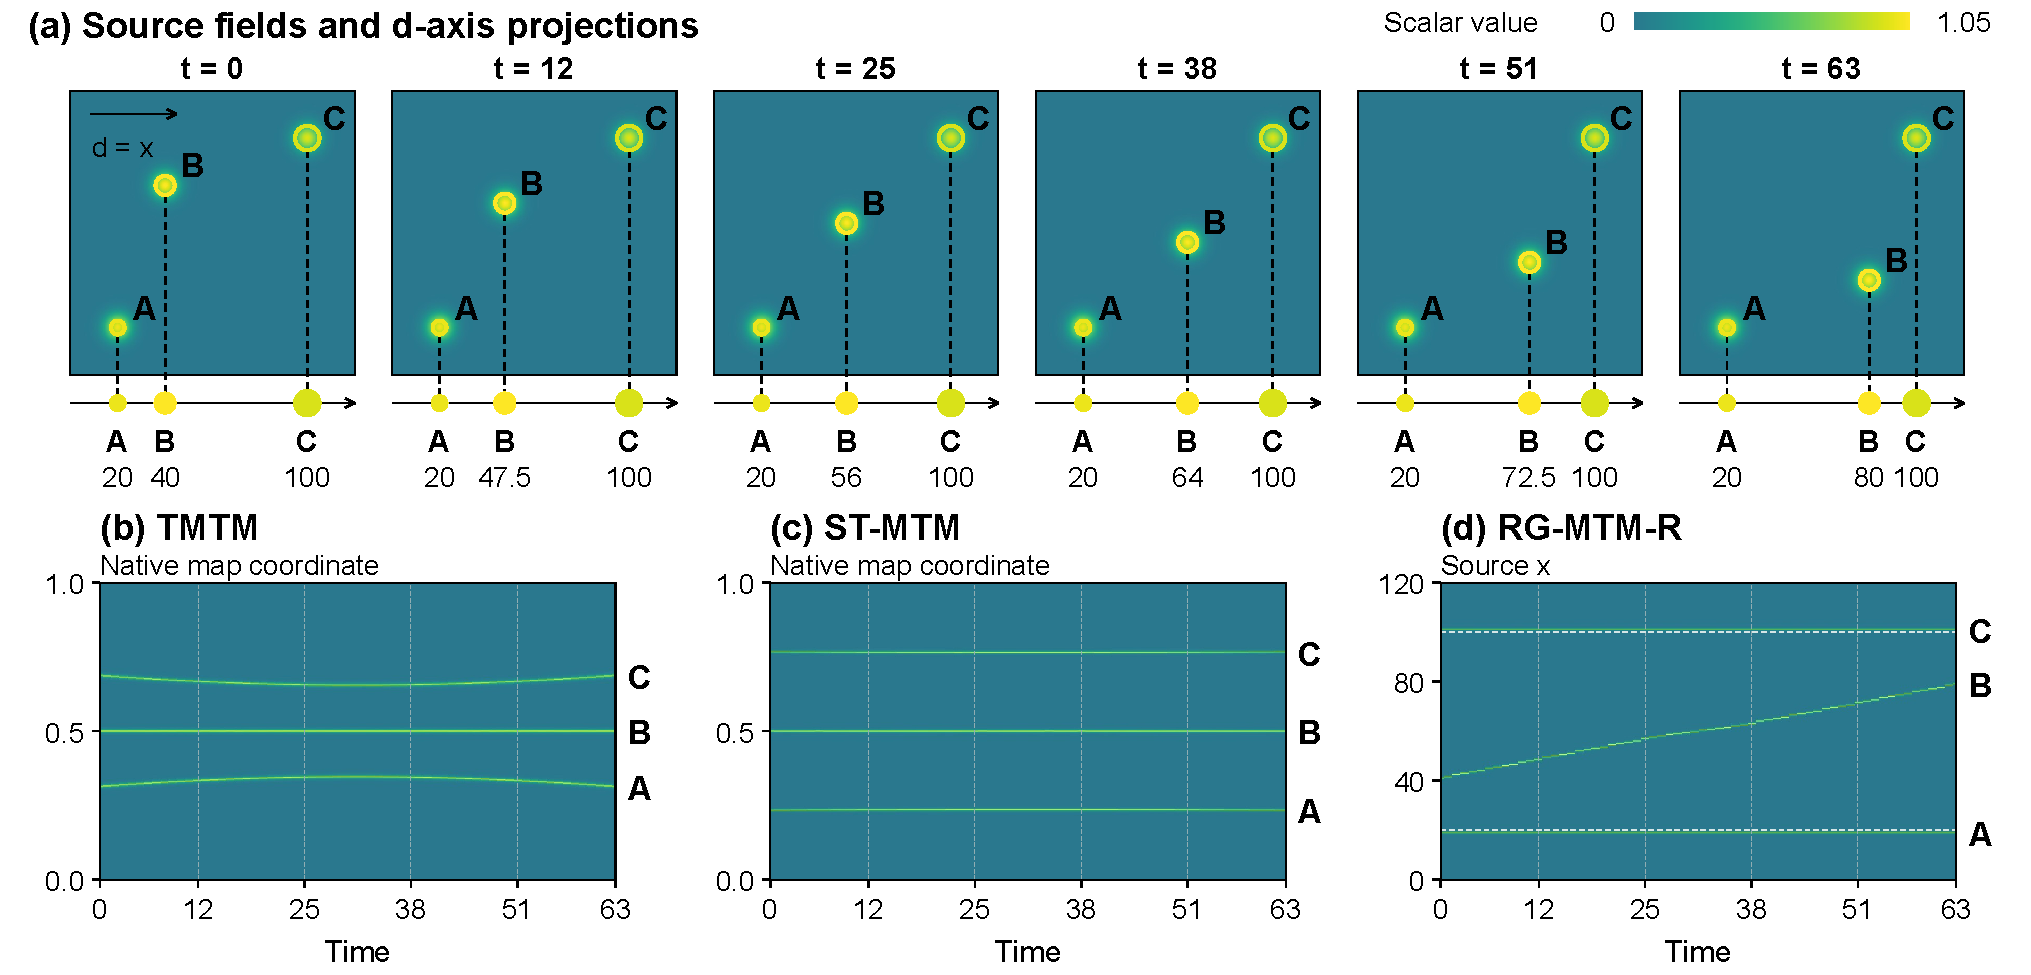
\includegraphics[width=\textwidth]{figures/Fig6.pdf}
\caption{Relative distances and absolute reference position. (a) Six source fields and $x$ projections follow moving $B$ between fixed $A,C$; mirror endpoints preserve pairwise distances while changing horizontal position. (b,c) TMTM/ST-MTM use internal map coordinates. (d) RG-MTM-R uses source $x$ units, with dashed fixed references. Source peaks and temporal bands share a linear 0--1.05 scalar scale. Vertical guides mark source-frame times. All three preserve merge levels; position errors and calibration are reported in Section~\ref{sec:reference_control}.}
\label{fig:bisector}
\end{figure*}

The mirror-motion control separates fixed-reference anchoring from pairwise-distance preservation (Fig.~\ref{fig:bisector}; protocol and measurements in Supplement S2, full visual comparison in S10). Across 64 fields on a $241^2$ grid, $B$ moves from $(40,80)$ to $(80,40)$ along the perpendicular bisector of fixed peaks $A=(20,20)$ and $C=(100,100)$. The mirror endpoints have identical distance matrices but different $q_i=x_i$. TMTM and ST-MTM keep $B$ near a constant map ordinate; RG-MTM-R follows its increasing reference. Final-frame position errors are 16.67\%, 16.67\%, and 0.84\%, using each baseline's best sequence-wide affine minimax calibration, including one global reflection. All three preserve merge levels. These 64 frames are independent of the 614-frame main suite.

\paragraph{Hierarchical row ordering.}
The certificate also diagnoses a clustering hierarchy of 1024 active wildfire cells, each containing 30 two-day observations. Optimal leaf ordering displaces some cells by 88.23\% of display height, compared with the hierarchy-constrained optimum of 67.29\% and the free-packing optimum of 20.55\%. Their separation distinguishes the chosen ordering from the cost imposed by subtree contiguity. Supplement S10 retains the full side-by-side display and protocol; S3 gives numerical precision and records.

\subsection{Data Size and Topological Complexity}
Spatial resolution determines the cost of tree extraction and the number of samples available for scalar filling; the number and branching degree of retained features determine the difficulty of positional diagnosis and order selection. Raster resolution controls how finely anchors and barriers appear in the final map. These are separate scales: a large input volume need not require exhaustive ordering of all its samples.

The retained binary-hierarchy benchmark increases from 64 leaves on 256 rows in 0.0041\,s to 4096 leaves on 16384 rows in 3.604\,s. These measurements concern positional diagnosis in the recorded benchmark environment. They do not include field preprocessing, scalar filling, or the quadratic layout. Exact small-tree frontiers enumerate permutations; flattening nodes can increase branching degree and the cost of subset-based diagnosis. The degree-controlled benchmark and timing details are in Supplement S3.


\section{Results}\label{sec:results}\label{sec:applications}
The results connect the quantitative comparisons to source-space interpretation. We first examine planar temporal maps, then a static slice and a sequence of static sections, followed by volumetric temporal data. Each comparison uses the same source features in P and R and reports the scalar connectivity exchanged for improved reference alignment. Temporal overviews, scalar profiles, and source views have distinct roles: they expose evolution, show connection thresholds, and locate features in the original domain, respectively.

% Declare the wide result figures before their discussion so that the
% two-column output routine can place them at the next page top.
\begin{figure*}[t]
\centering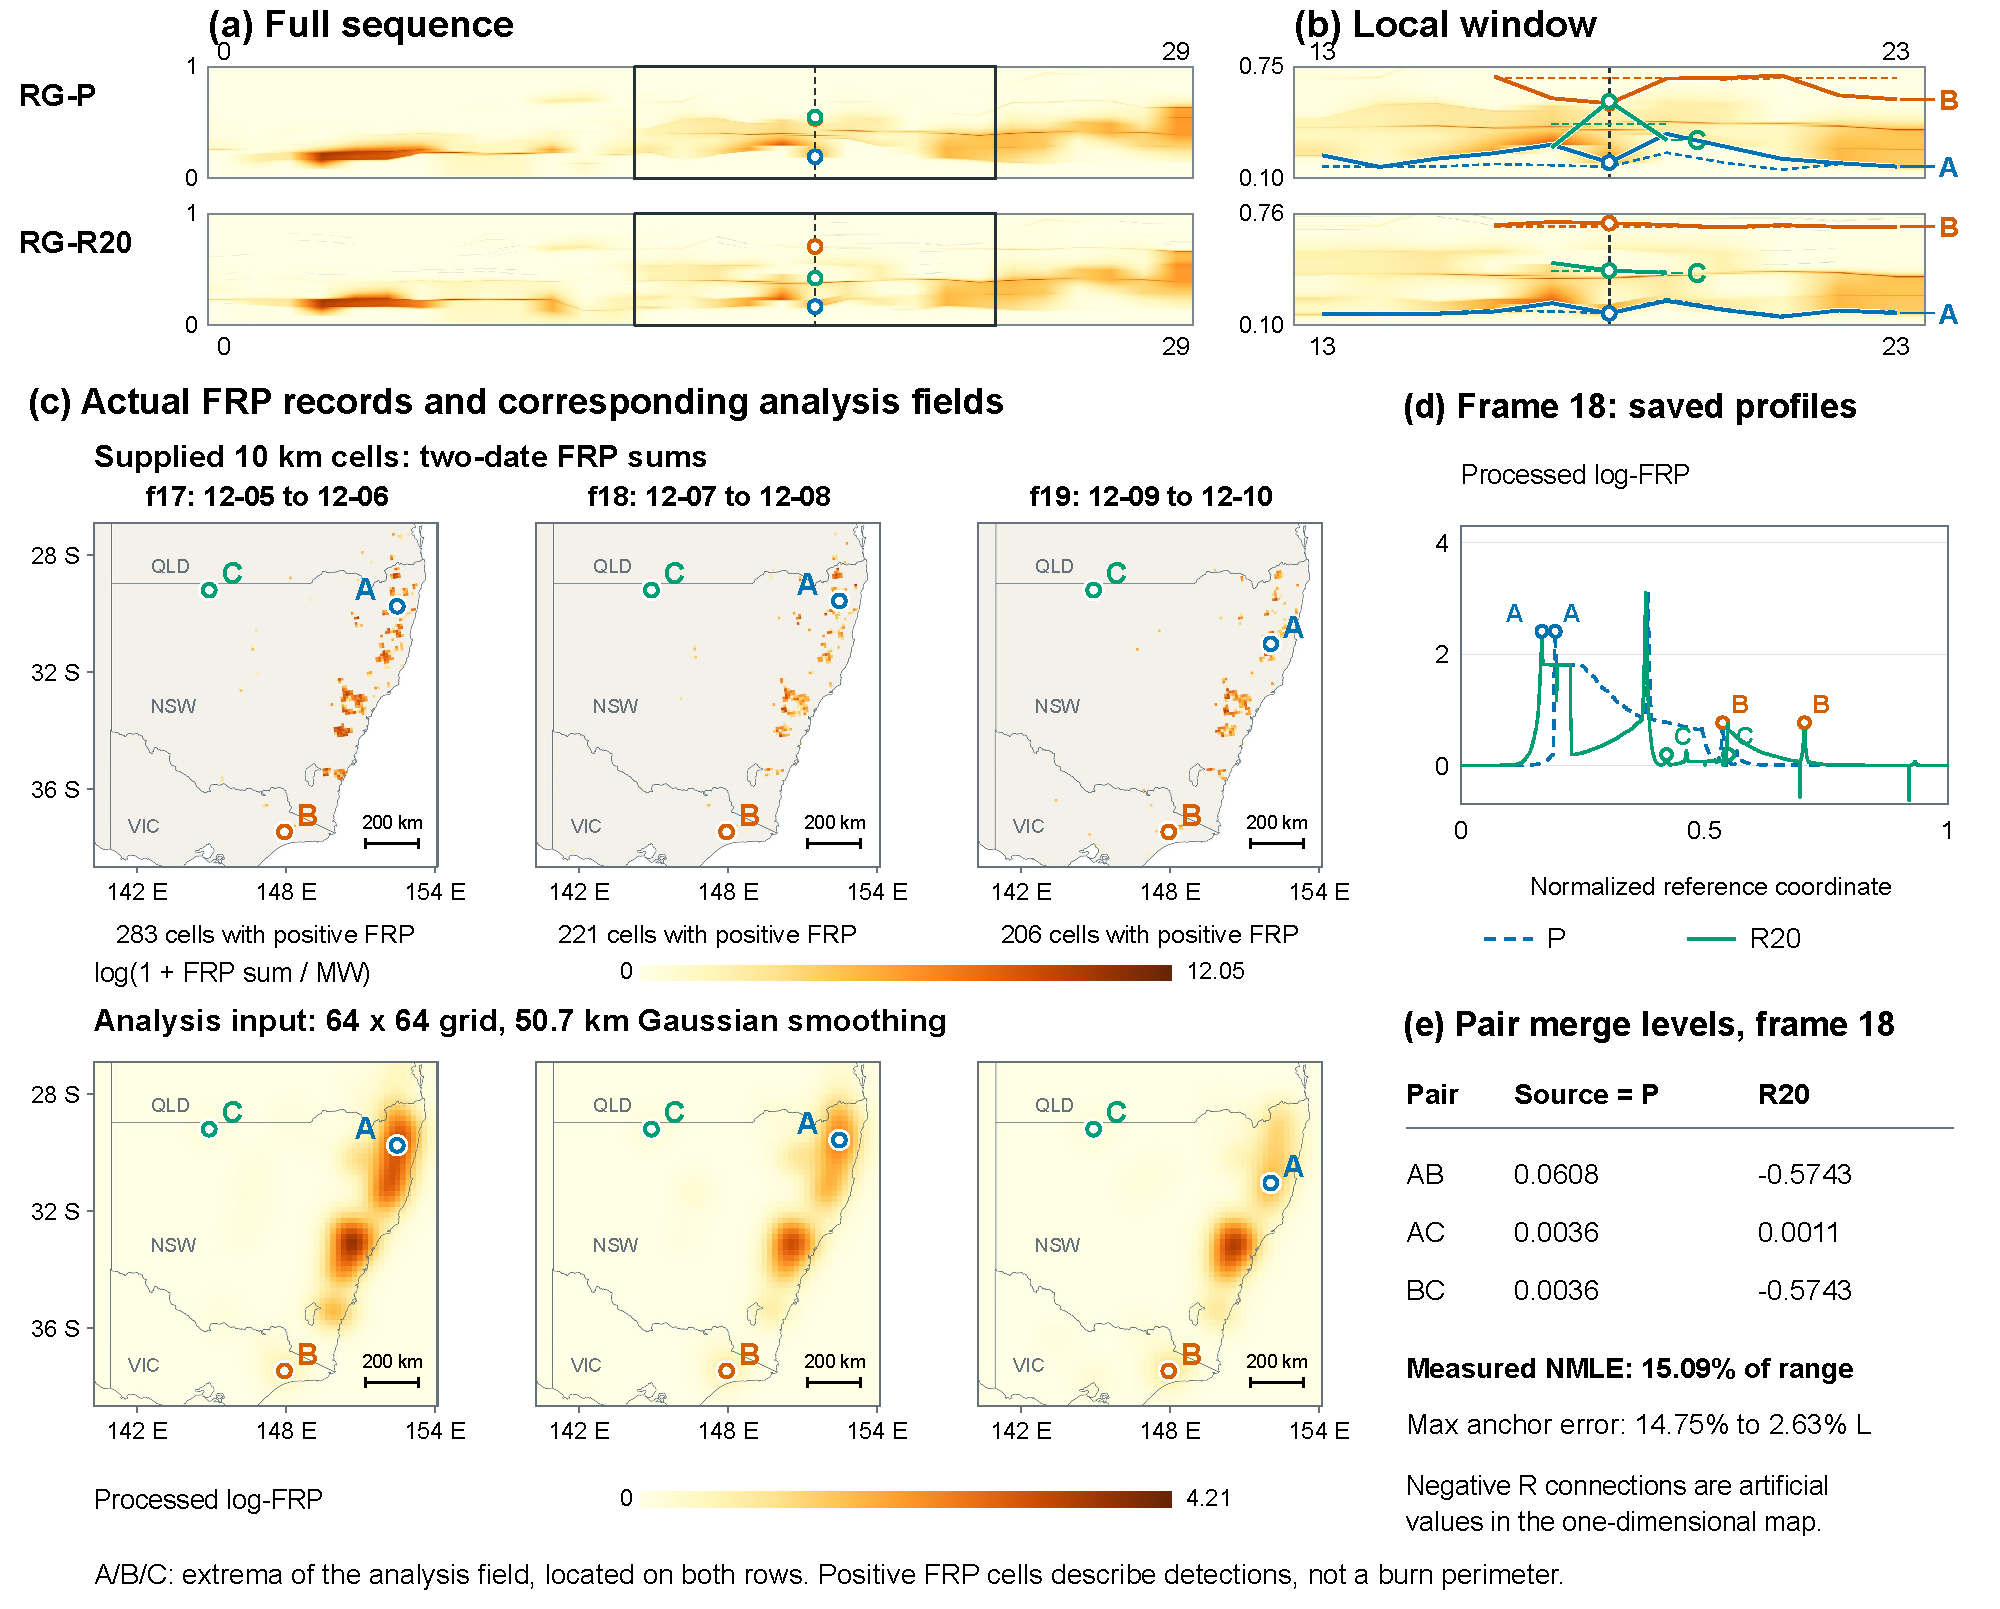
\includegraphics[width=\textwidth]{figures/Fig7.pdf}
\caption{Wildfires: RG-MTM-P/R over all 30 frames (a), with frames 13--23 enlarged (b). Panel (c), top: actual supplied 10-km FRP cell polygons for December 5--6, 7--8, and 9--10, 2019 (frames 17--19), on a geographic basemap~\cite{NaturalEarth:WildfireAdmin1}. Only cells with positive two-date FRP sums are colored; they indicate recorded fire activity rather than a burn perimeter. Bottom: the corresponding saved analysis fields, after aggregation onto a $64\times64$ grid (20.3-km cells), $\log(1+\mathrm{FRP}/\mathrm{MW})$, 50.7-km Gaussian smoothing, and the declared weak background. Both rows share the same extent, with geographic coordinates and 200-km scale bars. Tracks $A=3$, $B=48$, $C=52$ mark the same analysis extrema on both rows. Yellow--orange--brown uses fixed ranges 0--12.05 for supplied cells and 0--4.21 for processed fields and maps. Solid traces in (b) are anchors; dashed traces are references. At frame 18, relaxation reduces maximum displacement from 14.75\% to 2.63\% at 15.09\% actual NMLE. Panels (d)--(e) retain complete saved P/R scalar profiles and measured pair connection values. Negative connections are artificial map output, not negative observed FRP. This selected maximum-obstruction witness explains the mechanism; complete-sequence statistics and baseline panels are reported separately (Supplement S10). Temporal colour transitions use display interpolation only; saved frames, anchors, and evaluation samples are unchanged.}
\label{fig:fire_events}
\end{figure*}


\subsection{Two-Dimensional Data}\label{sec:results2d}
\subsubsection{Storms: Atmospheric Pressure}
Figure~\ref{fig:teaser} shows a separate hourly Storms visualization covering 1--31 December 1999 (744 hourly fields), using mean sea-level pressure anomalies relative to a centered 192-hour average. The analysis retains the fixed $49\times49$ grid, 250\,km smoothing and direction $d\approx(0.948,-0.319)$ estimated from the full sequence. The top R20 overview locates 2 December, 06:00--22:00 UTC and output positions $[0.10,0.42]$; its selected scalar columns are identical to R5. Five original-grid anomaly snapshots at 09:00, 10:00, 11:00, 13:00 and 18:00 locate the same processed extrema as the P/R1/R2/R5 maps. The fractions are eligibility controls $\kappa/\Delta_F$, not hard bounds on actual merge error. This visualization does not replace or extend the 118-frame half-day sequence used in the quantitative tables.

At 09:00, $A$ lies in the subtropical North Atlantic and $B$ near Iceland. Their projected references are $0.339L$ and $0.182L$, while P places them at $0.238L$ and $0.283L$, reversing their directional order. R5 restores that order with anchors $0.348L$ and $0.173L$. At 13:00, R1 restores the order of $A/C$; at 18:00, R2 restores $E/F$. The letter $E$ marks the computed minimum associated with the Anatol event context~\cite{Koepp:2023:TMTM}, rather than an independently validated physical track. The geographic position and directional reference of $A$ are unchanged between 09:00 and 10:00, but P moves its anchor by $0.110L$ as $B$ ceases to be an independent extracted extremum. R5 avoids this particular jump. The snapshots also explain why labels do not imply a continuous physical identity: $B$ is absent at 10:00 and 11:00, and the nearby extremum assigned track $C$ first appears at 12:00. Only features in the five displayed snapshots are marked in the lower maps. Supplement S8 records identities, source coordinates, the forward-prefix calculation and directly measured scalar costs.

In the separate 118-frame evaluation sequence, the 11 December 1999 case (Supplement S8) illustrates how geographic location and pressure connectivity interact. The source tree connects minima $A,B$ before the outside minimum $C$ joins, but the projection places $C$ between them. A preserving layout therefore moves at least one feature away from its reference. The certificate attributes $8.45\%$ of reference extent to this hierarchy obstruction. R admits the spatial order $A,C,B$ and places the marked tracks close to their source references. Across all five features at this time, maximum displacement decreases from 8.87\% for P to 0.83\% for R. The corresponding TMTM, ST-MTM, P, and R panels are retained in Supplement S8.

The improved alignment has an interpretable scalar price. The $A/B$ connection changes from approximately 994.1 to 1006.7\,hPa, while its connections to $C$ change from 1009.4 to 1006.7\,hPa. These are the pressure thresholds at which the displayed components connect. The worst-pair change is 12.558\,hPa, or 13.21\% actual NMLE; the complete-sequence mean is 1.47\%. Thus, the map exposes both the geographic order gained by relaxation and the pressure-connectivity detail exchanged for it. Supplement S8 provides the full frame-level measurements and analytical-versus-rendered costs.

% Declare the remaining planar figures before their discussion.
% Static planar figures are declared after the temporal comparisons.

\subsubsection{Wildfires: Fire Radiative Power}
The Wildfires sequence summarizes fire-radiative-power observations in 30 two-day intervals. Figure~\ref{fig:fire_events} shows stronger processed fire activity as orange--brown bands against the pale lower-valued background. Panel (c) distinguishes the supplied 10-km cell records from the smoothed fields used to construct the trees. The supplied polygons retain their actual geometry and sparse support: frames 17--19 contain 283, 221, and 206 cells with positive two-date sums. Coastlines, state boundaries, coordinates, and scale bars locate them in southeastern Australia. The lower row shows the unchanged analysis input, including the declared 50.7-km smoothing; its continuous regions do not establish continuous burning or a fire boundary. Both rows locate the same processed extrema $A$, $B$, and $C$, while both RG maps use the same fixed spatial reference. Supplement S10 retains the TMTM and ST-MTM panels with their native coordinates.

Frames 17--19 illustrate why this distinction matters. The projected location of feature $C$ stays fixed, yet its P band shifts upward at frame 18 and returns in the next observation. The R band stays close to the same reference through all three frames. The spatial snapshots and matching labels separate this layout-induced displacement from a change in the feature's observed reference position. The comparison concerns the same overlap-linked features and the same scalar observations.

At frame 18, the source hierarchy groups $A,B$ while the reference requests $A,C,B$. Relaxation reduces maximum displacement from 14.75\% to 2.63\% of reference extent. The connecting scalar profile changes as well: R lowers the $A/B$ barrier from 0.060800 to $-0.574262$ in processed log-FRP units. The grey-blue under-range colour shows this artificial connection level alongside the improved anchor alignment. The resulting actual NMLE is 15.09\%; the original fire observations remain nonnegative. Exact coordinates, orders, and costs are recorded in Supplement S7--S8.

At the selected frame, the complete profiles and pair table in Fig.~\ref{fig:fire_events}(d)--(e) make the scalar price explicit: the $A/B$ connection changes from 0.060800 in the source and P to $-0.574262$ in R20. This artificial negative connection yields the measured 0.635063 worst-pair change. The frame is a selected maximum-obstruction witness among the tracked three-feature conflicts, rather than a typical-case claim.

\begin{figure}[tb]
\centering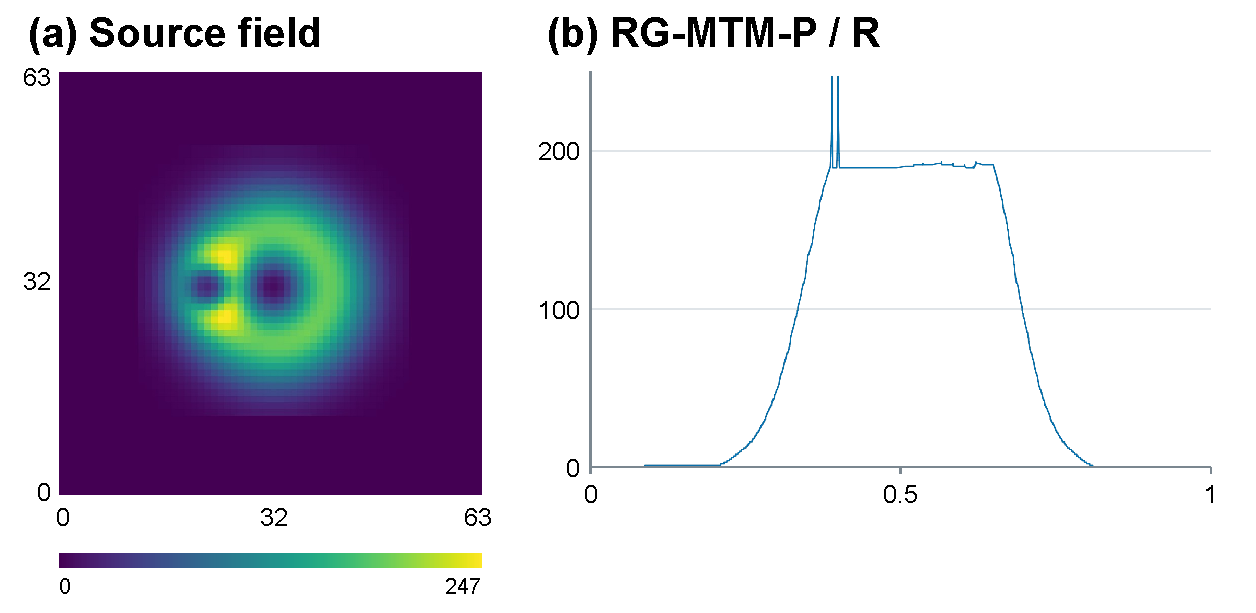
\includegraphics[width=\linewidth]{figures/Fig8.pdf}
\caption{Nucleon: the unchanged author $64\times64$ scalar slice (a) and the complete RG-MTM-P profile (b, 32768 samples). Every R setting returns exactly the same profile as P. Both panels retain the original scalar units. NROE is 2.38\%, with zero measured NMLE. This is one static slice; the TMTM comparison is in Supplement S10.}
\label{fig:nucleon}
\end{figure}

\begin{figure*}[t]
\centering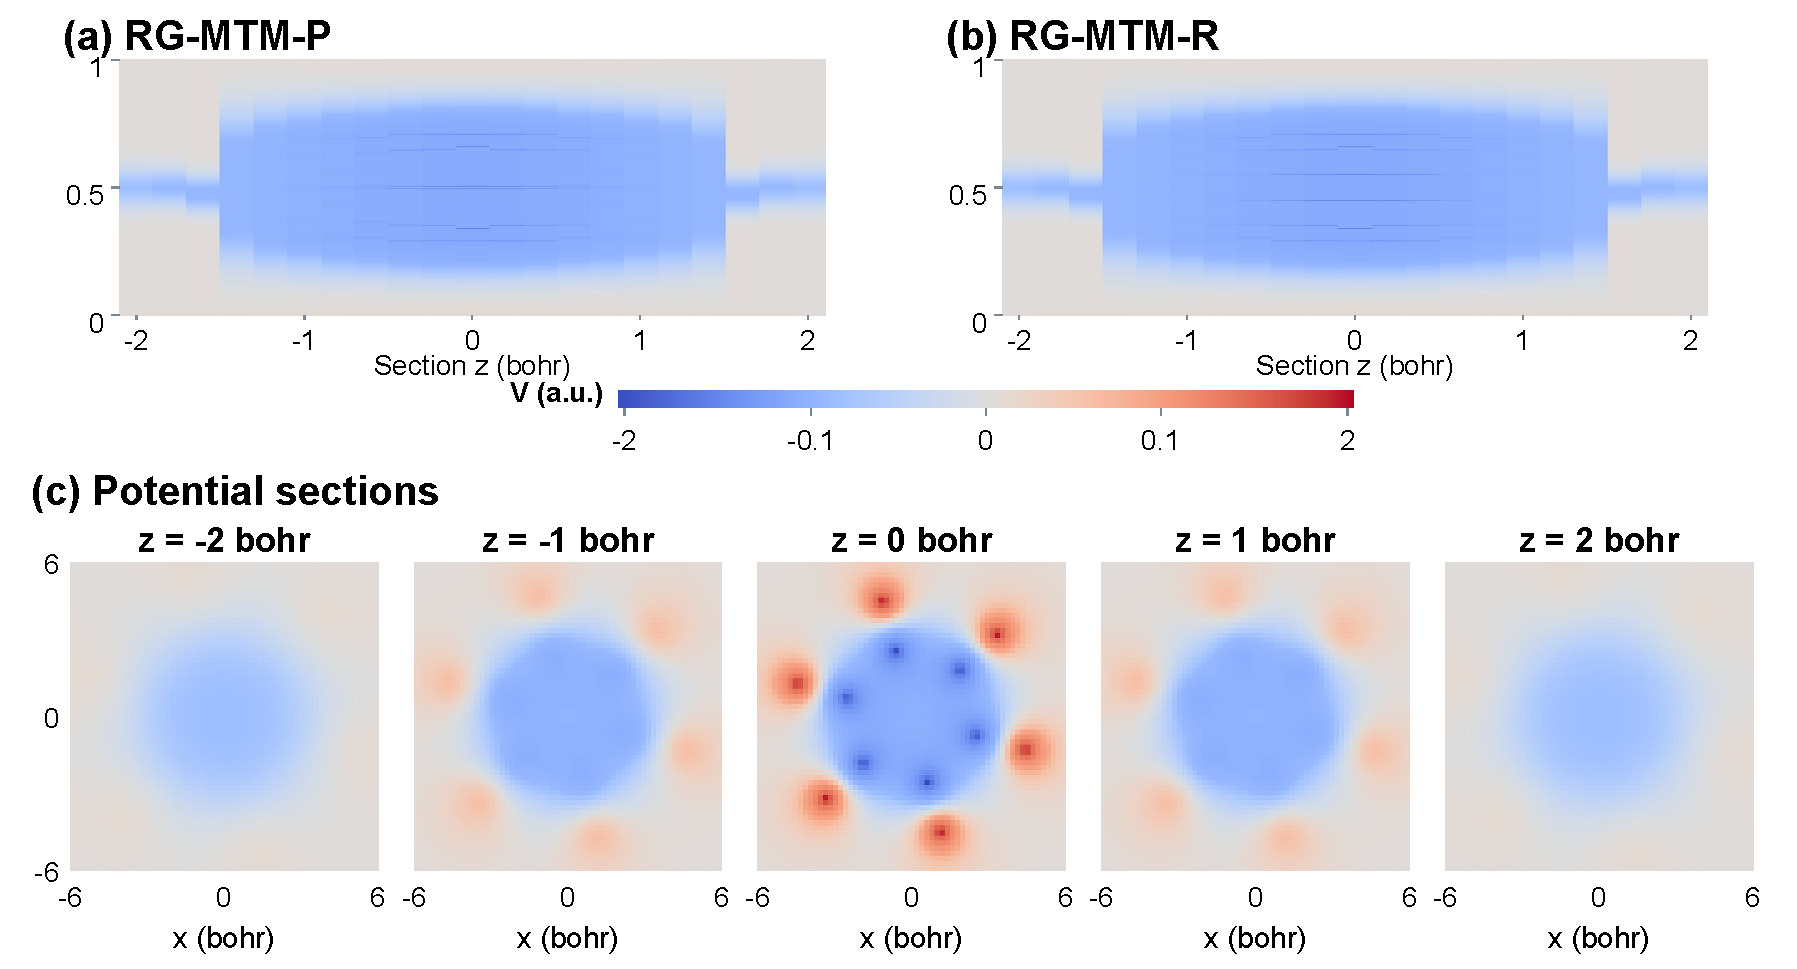
\includegraphics[width=\textwidth]{figures/Fig9.pdf}
\caption{Benzene: RG-MTM-P/R2 maps of all 21 static $z$ sections (a,b), with source potential at $z=-2,-1,0,1,2$ bohr (c). Section $z$ is a spatial coordinate. Maps and source fields share a symmetric-log scale, linear within $\pm0.0784$ a.u.; potential is in Hartree/$e$. This is the declared OPLS-AA reconstruction. The TMTM comparison is in Supplement S10; full and interior-extremum scores are in S9.}
\label{fig:benzene}
\end{figure*}

\subsubsection{Nucleon: Static Scalar Structure}\label{sec:nucleon}
Nucleon tests a static layout on the TMTM authors' original padded $64\times64$ scalar slice~\cite{Koepp:2023:TMTM}. Figure~\ref{fig:nucleon} pairs the complete source slice (a) with the complete P/R scalar profile (b). Both panels describe the same static input. The input has one frame and 13 extracted extrema; the derived tree has 26 nodes, compared with 28 in the reference table. The source samples are unchanged, and no simplification threshold is applied. TMTM has 11.90\% NROE, while P has 2.38\%; both have zero measured NMLE. Table~\ref{tab:tradeoff} group its order, merge-level, and displacement measurements with the other planar inputs. All three R settings return exactly the same saved profile as P, so relaxation adds no benefit in this case. This null relaxation result shows that reference guidance can improve a legal order without requiring a scalar trade-off. The added ST-MTM run has 11.90\% NROE and zero NMLE; its stronger SNS/TW (Table~\ref{tab:tradeoff}) shows that this static reference-order gain does not imply a relative-geometry gain. The example supplies a static scalar comparison; its single slice supports neither temporal nor volumetric claims.

\subsubsection{Benzene: Reconstructed Electrostatic Potential}\label{sec:benzene}
The Benzene experiment uses an explicitly reconstructed electrostatic potential, rather than the unavailable original author file. An OPLS-AA point-charge model assigns $-0.115e$ to each carbon and $+0.115e$ to each hydrogen~\cite{Jorgensen:2013:BOSS}. Atomic positions come from the header of a public Inviwo molecular cube~\cite{Inviwo:BenzeneGeometry}; its electron-density samples are not used. We evaluate $V(r)=\sum_iq_i/\|r-R_i\|$ on 21 parallel $61\times61$ sections, with $x,y\in[-6,6]$ and $z\in[-2,2]$ in bohr. Section $z$ is a spatial coordinate of a static field, not physical time. This classical reconstruction is a model-specific comparison, not the original fractional-charge potential or a quantum-chemical reproduction.

Figure~\ref{fig:benzene} pairs the P/R slice maps with five source sections; Supplement S10 retains the full baseline comparison. Join trees retain low-potential extrema after a common 0.05\% per-section persistence simplification. P reduces mean NROE from 50.00\% to 4.21\% while preserving merge levels. Each R setting reaches zero NROE with 0.0025\% mean and 0.0080\% maximum NMLE; the three settings have identical measured results. The added ST-MTM run also has 50.00\% mean NROE and zero NMLE, with lower SNS than P/R but larger adjacent-section displacement than R. Neither TMTM nor ST-MTM optimizes the supplied $x$ reference, so these values assess reference compatibility rather than its original objective.

Four boundary extrema occur in every section and contribute substantially to the complete-leaf score. On the 15 sections with at least two interior extrema, interior-only NROE is 12.50\% for TMTM, 5.89\% for P, and zero for R. Across 170 overlap matches, mean adjacent-section displacement residual is 2.755\% for TMTM, 1.219\% for P, and 0.137\% for R. Mean $\pm z$ map discrepancy similarly changes from 0.0185\% to 0.0064\% to 0.0030\%. The source field is only approximately mirror-symmetric: its maximum paired discrepancy is 0.0241\% of scalar range. These are slice-coherence diagnostics, not molecular-motion errors (Supplement S9). Keeping the boundary and full-population results together makes the scope of the apparent position gain explicit.

% Finish all planar result panels before the volumetric group.
\FloatBarrier
\subsection{Three-Dimensional Data}\label{sec:results3d}
\begin{figure*}[t]
\centering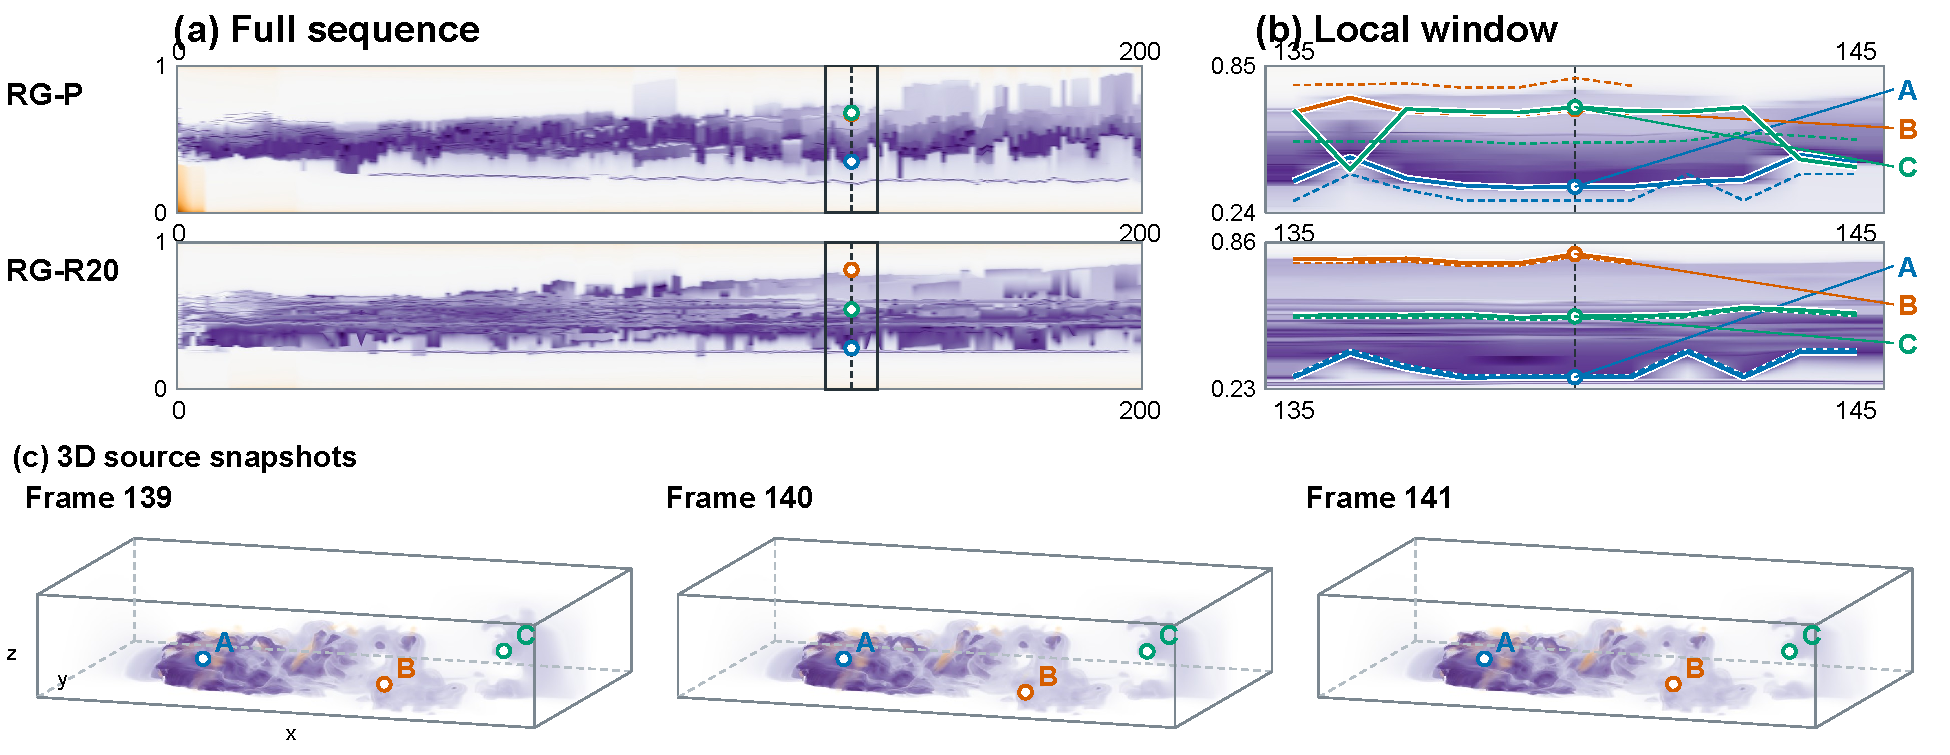
\includegraphics[width=\textwidth]{figures/Fig10.pdf}
\caption{Tangaroa: RG-MTM-P/R20 across all 201 original-grid fields (a), the local window 135--145 (b), and full-volume views at frames 139--141 (c). Tracks $A=432$, $B=462$, $C=388$ link saved anchors, dashed references, and true three-dimensional extrema. The common orthographic camera and domain frames preserve spatial context. The retained purple--white--orange speed transfer function uses $[0,2]$. At frame 140, P/R maximum displacement is 14.76\%/1.02\%, with 13.75\% actual R NMLE. Full baseline panels and rendering details are in Supplement S6, S8, and S10. Temporal colour transitions use display interpolation only; saved frames, anchors, and evaluation samples are unchanged.}
\label{fig:volume}
\end{figure*}

\begin{figure*}[t]
\centering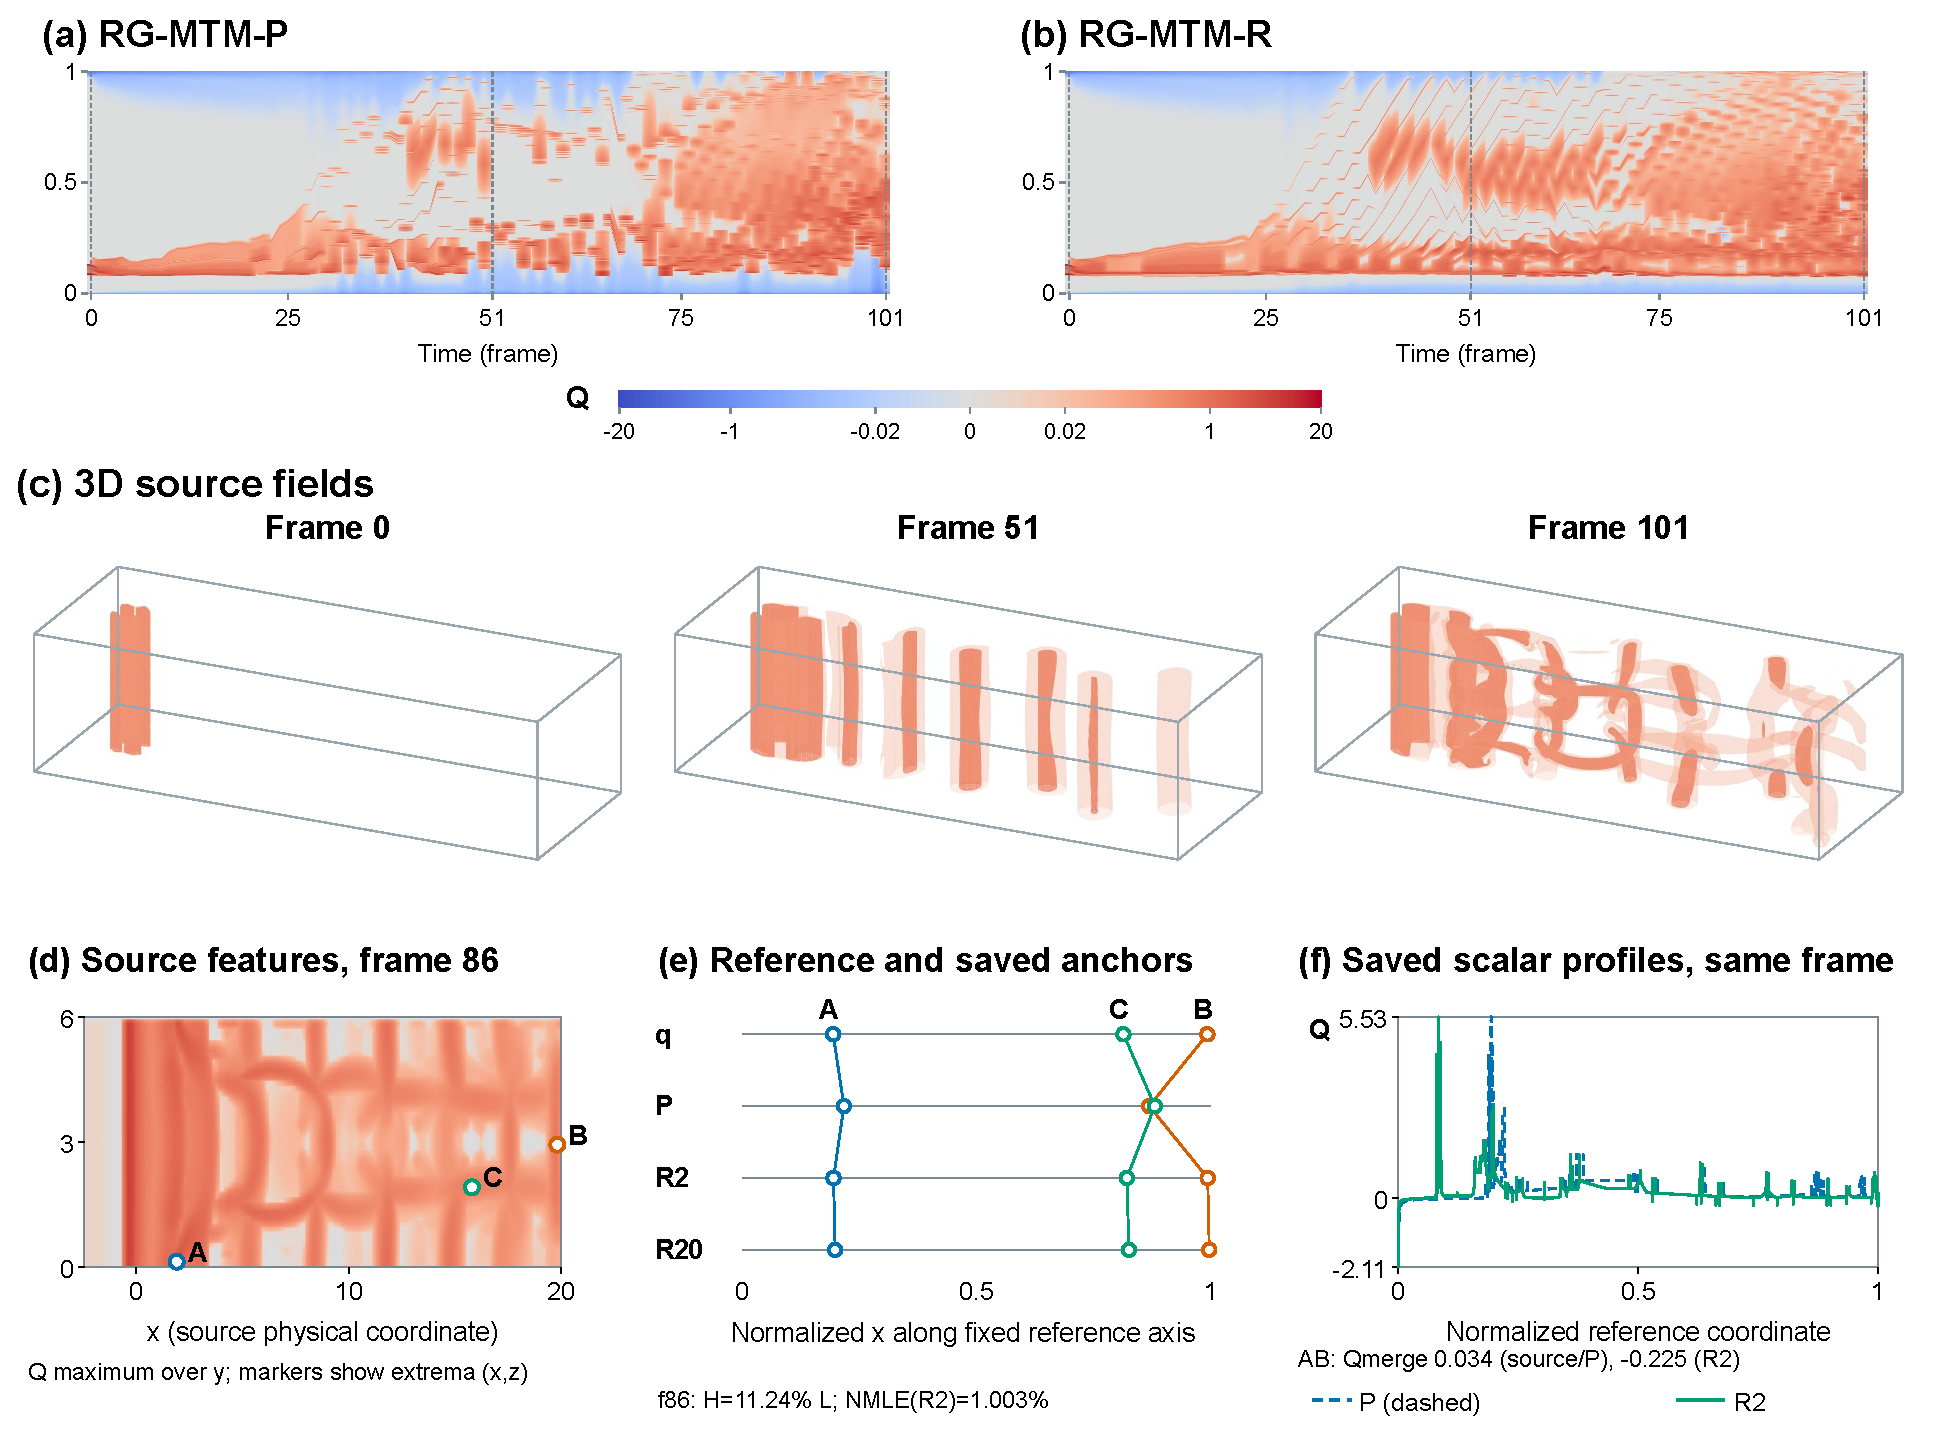
\includegraphics[width=\textwidth]{figures/Fig11.pdf}
\caption{Cylinder: RG-MTM-P (a) and R20 (b) for all 102 original-grid three-dimensional $Q$ fields, with source isosurfaces at frames 0, 51, and 101 (c). The maps use normalized physical $x$ reference position; vertical guides locate the source views. Their common symmetric-log colour scale is linear within $\pm0.02$. Isosurfaces at $Q=0.1$ (translucent) and $0.5$ (solid) share physical aspect, camera, and domain frame. Source views precede persistence simplification; maps use the common simplified inputs. Full TMTM/R2 panels and rendering details are in Supplement S9--S10. Panels (d)--(f) link a median-criterion selected conflict at frame 86 to its source features, continuous anchors and complete P/R2 profiles. Maximum displacement changes from 12.40\% to 1.17\% of reference extent, with 1.003\% R2 NMLE. The local case is descriptive; full-sequence scores remain in the common tables. The source projection in (d) uses bilinear display reconstruction with exact original cell centers. Temporal colour transitions use display interpolation only; saved frames, anchors, and evaluation samples are unchanged.}
\label{fig:cylinder}
\end{figure*}

\paragraph{Completed volumetric baseline and geometry comparison.}
All 303 volumetric inputs now have native ST-MTM layouts and the same SNS/TW/TD evaluation as the planar data (Table~\ref{tab:tradeoff}). On Tangaroa, ST-MTM reduces SNS from TMTM's 0.5255 to 0.1655 and increases TW from 0.6701 to 0.8137. Its NROE is 21.34\%, compared with P's 9.61\% and R20's 0.019\%, while its TD is 138.55 versus TMTM's 64.86 and R20's 39.71. Relative-distance quality, reference alignment and temporal stability therefore give different rankings on this sequence.

On Cylinder, ST-MTM reduces TMTM's NROE from 26.62\% to 17.77\%, SNS from 0.2956 to 0.1346 and TD from 85.03 to 43.17. R20 has lower NROE (0.084\%), SNS (0.0399) and TD (29.11), but slightly lower TW (0.8912 versus ST-MTM's 0.8989) and nonzero merge-level cost. ST-MTM makes 4730/6755 Tangaroa and 1469/3196 Cylinder motion errors under each dataset's retained threshold protocol; P/R20 make 3697/2060 and 1191/605, respectively. These are within-dataset geometric proxies, not pooled accuracies. All new ST-MTM profiles preserve source pairwise merge levels exactly. Supplement S3 documents the fixed generic extension and its solver/width certificates.

\subsubsection{Tangaroa: Velocity Magnitude}\label{sec:volume}
Tangaroa describes airflow around a research vessel, whose geometry influences the surrounding flow~\cite{Popinet:2004:Tangaroa,Koepp:2023:TMTM}. Figure~\ref{fig:volume} combines temporal maps of all 201 velocity-magnitude fields with full-volume views. The maps compress the spatial domain into a fixed projected axis and expose the retained low-speed features across time; the volume views provide the three-dimensional context needed to locate those features around the vessel. All layouts use the same original-grid fields and fixed 10\% persistence setting described below and in Supplement S6.

Tangaroa contains 201 velocity fields on the original $300\times180\times120$ grid, with time increment 0.01~\cite{Popinet:2004:Tangaroa}. Velocity magnitude is computed in float64 and stored as float32; magnitudes below $10^{-6}$ are replaced by 1 and the values clipped to $[0,2]$. TTK 0.9.9~\cite{Tierny:2018:TTK} applies traditional simplification at absolute persistence 0.2, followed by augmented join-tree extraction. This fixed 10\% setting retains 18--93 leaf features per frame. We compare TMTM, the completed ST-MTM extension, P, and R at eligibility fractions 2\%, 20\%, and 100\%. The 201-frame population is independent of the planar suite; the common continuous displacement definition is given in Section~\ref{sec:eval}; Supplement S6 retains the complete protocol and the separate rendered-anchor diagnostic.

The complete temporal maps show the effect of reference guidance on the arrangement of the bands. P preserves the source merge levels while reducing mean NROE from TMTM's 20.09\% to 9.61\%. R20 follows the reference order more closely, reaching 0.019\% mean NROE and 1.176\% pooled continuous anchor error. This arrangement incurs 14.44\% mean and 31.02\% maximum NMLE. Supplements S6 and S9 retain the intermediate R2 setting, R100, and the separately evaluated three-dimensional and projected motion decisions.

The snapshots at frames 139--141 connect this sequence-level change to individual source features. At frame 140, the source join tree groups $A,B$, whereas the reference places $C$ between them. P orders the marked features $A,B,C$, while R20 uses $A,C,B$; the TMTM order $C,A,B$ is shown in Supplement S10. The markers in the volume views and local temporal windows identify the same retained extrema. Maximum P/R displacement over all 27 features falls from 14.76\% to 1.02\% of reference extent, with 13.75\% actual NMLE. The local profile changes the $A/B$ and $A/C$ connection levels by 0.275004 in speed units, making the price of the spatial reordering explicit.

Shared markers connect the sequence-wide reference map to source extrema and their changed connection levels. Supplement S8 gives the coordinates and diagnostics; S6 verifies complete volumes, certificate bounds, and rendered profiles.

Tangaroa's 18--93 retained features per frame require continuous bounds and a finite candidate search rather than complete order enumeration. The large-tree solver retains certificate bounds and evaluates at most four candidate-order QPs; R2 has 48 open certificate intervals. Actual errors are measured on complete 131072-row profiles, while the 4096-row preview can omit narrow visible bands. Supplement S6 records these solver and display resolutions.

\subsubsection{Cylinder: Three-Dimensional Vortex Activity}\label{sec:cylinder}
Cylinder extends the volumetric evaluation to the direct numerical square-cylinder flow of Camarri et al.~\cite{Camarri:2005:Cylinder}, uniformly resampled by Weinkauf~\cite{Weinkauf:SquareCylinder,Funck:2008:Smoke}. All 102 public velocity volumes are used. We compute the three-dimensional $Q=\tfrac12(\|\Omega\|_F^2-\|S\|_F^2)$ on the $192\times64\times48$ velocity grid before retaining the author's $135\times64\times48$ downstream subdomain. The input is volumetric at every time, without spatial downsampling, smoothing, or feature-count selection. The 102 available times differ from the 508 reported in TMTM; this is a corresponding public-data experiment rather than a replication of its final derived input.

Figure~\ref{fig:cylinder} relates the P/R20 complete-sequence maps to three-dimensional source isosurfaces at frames 0, 51, and 101. A fixed $x$ reference permits comparison of downstream feature positions. The source views show the spatial distribution of positive-$Q$ structures, while the maps expose how their scalar patterns are arranged over the sequence. Persistence simplification is fixed at 2\% of each frame's range, yielding 4--75 retained extrema; it is distinct from the RG relaxation eligibility parameter. The unified evaluation tables include Cylinder with all other inputs; Supplements S9--S10 retain all five configurations and the full visual comparison.

P decreases mean NROE from 26.62\% to 12.26\% with zero measured NMLE. R2 reaches 0.249\% NROE at 0.692\% mean and 4.886\% maximum NMLE; R20 reaches 0.084\% NROE at 2.810\% mean and 14.281\% maximum NMLE. R100 has the same mean NROE as R20 but greater mean scalar cost (3.190\%). Thus, wider relaxation eligibility does not ensure a preferable measured trade-off.

For 3196 clear three-dimensional approach/separation events, errors decrease from 2141 for TMTM to 1191 for P and 605 for R20 (66.99\%, 37.27\%, and 18.93\%). Exact $x$ projection still makes 603 errors (18.87\%), identifying spatial information lost in projection. The corresponding projected-event rates use a different denominator, 2934 events: R20 makes 108 errors (3.68\%). These overlap-based geometric proxies do not establish physical vortex identities. Supplement S9 supplies the complete counts, boundary treatment, and solver records.


Figure~\ref{fig:cylinder}(d)--(f) follows a conflict at frame 86 selected by the median obstruction/gain criterion across 85 eligible frames. The source image takes the maximum $Q$ over $y$ and projects the same original three-dimensional extrema onto $(x,z)$; it does not replace the volumetric input with a planar field. P orders the marked features $A,B,C$, whereas the reference and R2 place $C$ between $A,B$. R2 lowers the frame's maximum displacement from 12.40\% to 1.17\% of $L$, at 1.003\% NMLE. The $A/B$ merge changes from 0.034060 to $-0.224935$ in $Q$ units. The local profiles use R2, while the overview maps and common primary tables use R20.

\subsection{OLR, PM2.5, and Ring: Complete Temporal Maps}\label{sec:remaining_temporal}
\begin{figure*}[t]
\centering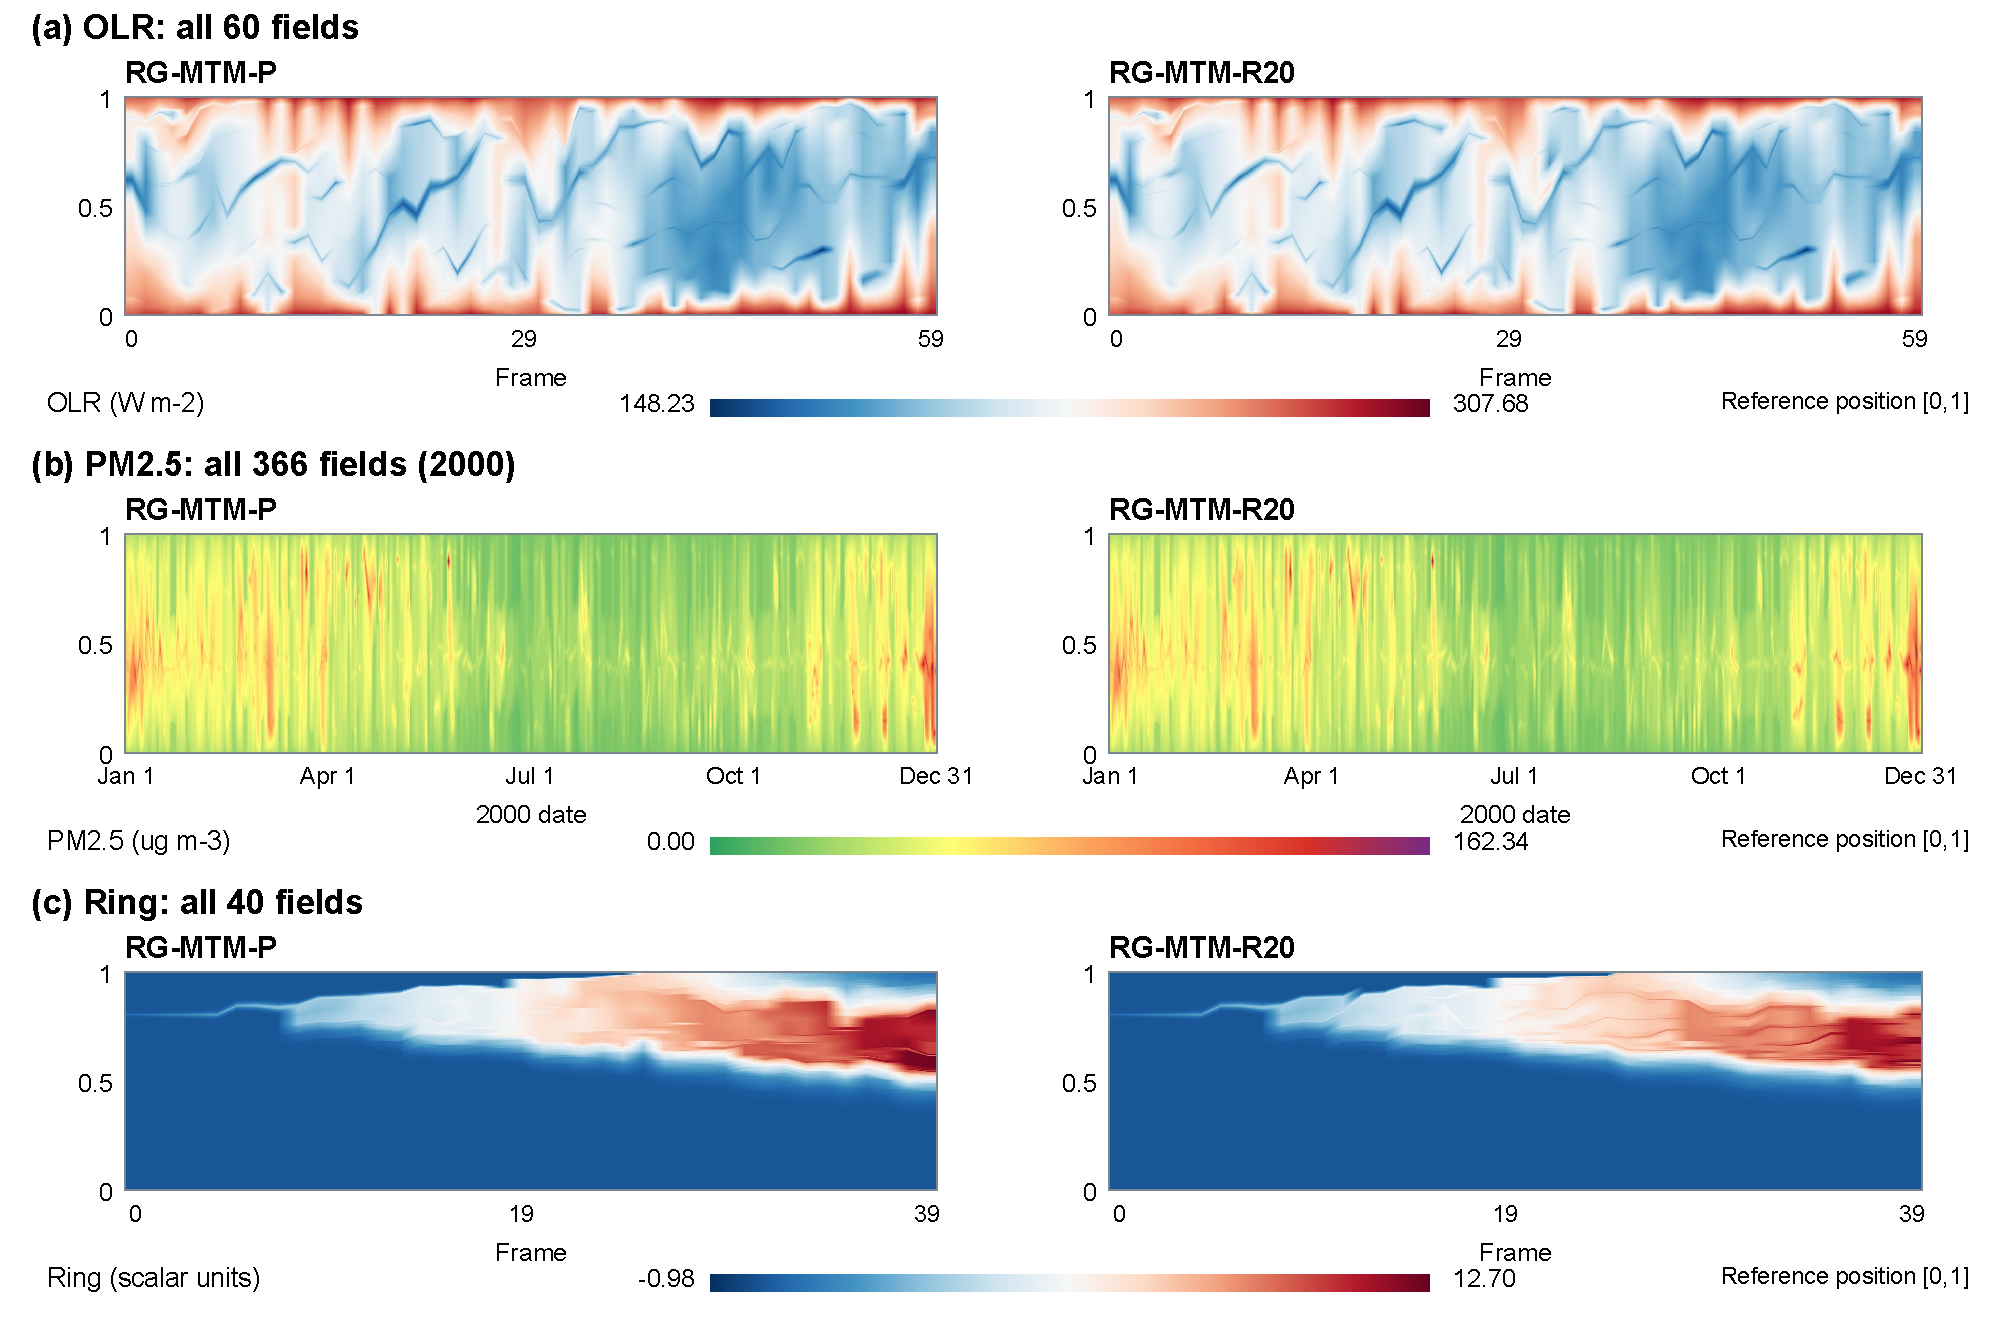
\includegraphics[width=\textwidth]{figures/Fig12.pdf}
\caption{Complete P/R20 temporal maps for three additional inputs: (a) OLR, all 60 daily fields; (b) PM2.5, all 366 fields in 2000; (c) Ring, all 40 synthetic fields. Horizontal axes show frames; vertical axes show the same normalized fixed reference within each P/R pair. Scalar ranges are shared within each row and independent between datasets. Maps use complete sequences without temporal cropping. Conservative display interpolation preserves each saved profile exactly; intermediate columns do not add observations. PM2.5 uses the user-authorized green--yellow--orange--red--purple pollution palette in concentration units, without AQI thresholds. Colours encode processed scalar values; any below-input-range connections are layout outputs. Complete arrays, not preview pixels, determine the reported errors. The complete four-method comparisons are in Supplement S10.}
\label{fig:remaining_temporal}
\end{figure*}

Figure~\ref{fig:remaining_temporal} completes the direct result coverage of all nine inputs. It shows all 60 OLR fields, all 366 PM2.5 fields in 2000, and all 40 Ring fields for P and R20. Each pair shares one fixed reference axis and scalar scale. Supplement S10 retains complete four-method comparisons with the baselines' native ordinates.

OLR NROE decreases from P's 0.89\% to zero, while motion errors remain 3/56. Annual PM2.5 NROE decreases from 0.9785\% to 0.0074\%; pooled displacement decreases from 1.87\% to 0.76\%, at 0.182\% mean and 4.669\% maximum NMLE. However, motion errors increase from 42/95 to 47/95. The complete year therefore supports reference alignment rather than a general improvement in spatial motion. January's selected seven-event example is retained only as a historical control. Ring reduces NROE from 2.66\% to 0.13\% and motion errors from 39/124 to 16/124, at 2.73\% mean NMLE.

Map appearance depends on temporal sampling, the number of retained extrema, and scalar filling. A frame with one or two extrema naturally contains broad bands; the full year adds observed temporal coverage without inventing additional features. For display in Figures~\ref{fig:fire_events}, \ref{fig:volume}, \ref{fig:cylinder}, \ref{fig:remaining_temporal}, and \ref{fig:pm25_case}, we interpolate neighbouring saved profiles with a monotone warp aligned to common extrema when order and displacement permit, otherwise using fixed-position linear interpolation. Every saved scalar profile remains exact at its frame before pixel rendering, and no scalar overshoot is introduced. For the Wildfires, Tangaroa, and Cylinder revisions, vertical area antialiasing integrates all stored rendering rows. The actual FRP cell polygons retain their discrete geometry. Intermediate columns are display samples, not additional observations, layouts, or temporal evidence. All numerical results use the original saved frames.

\subsubsection{PM2.5: Annual Context and a Source-Linked Case}\label{sec:pm25_case}
\begin{figure*}[t]
\centering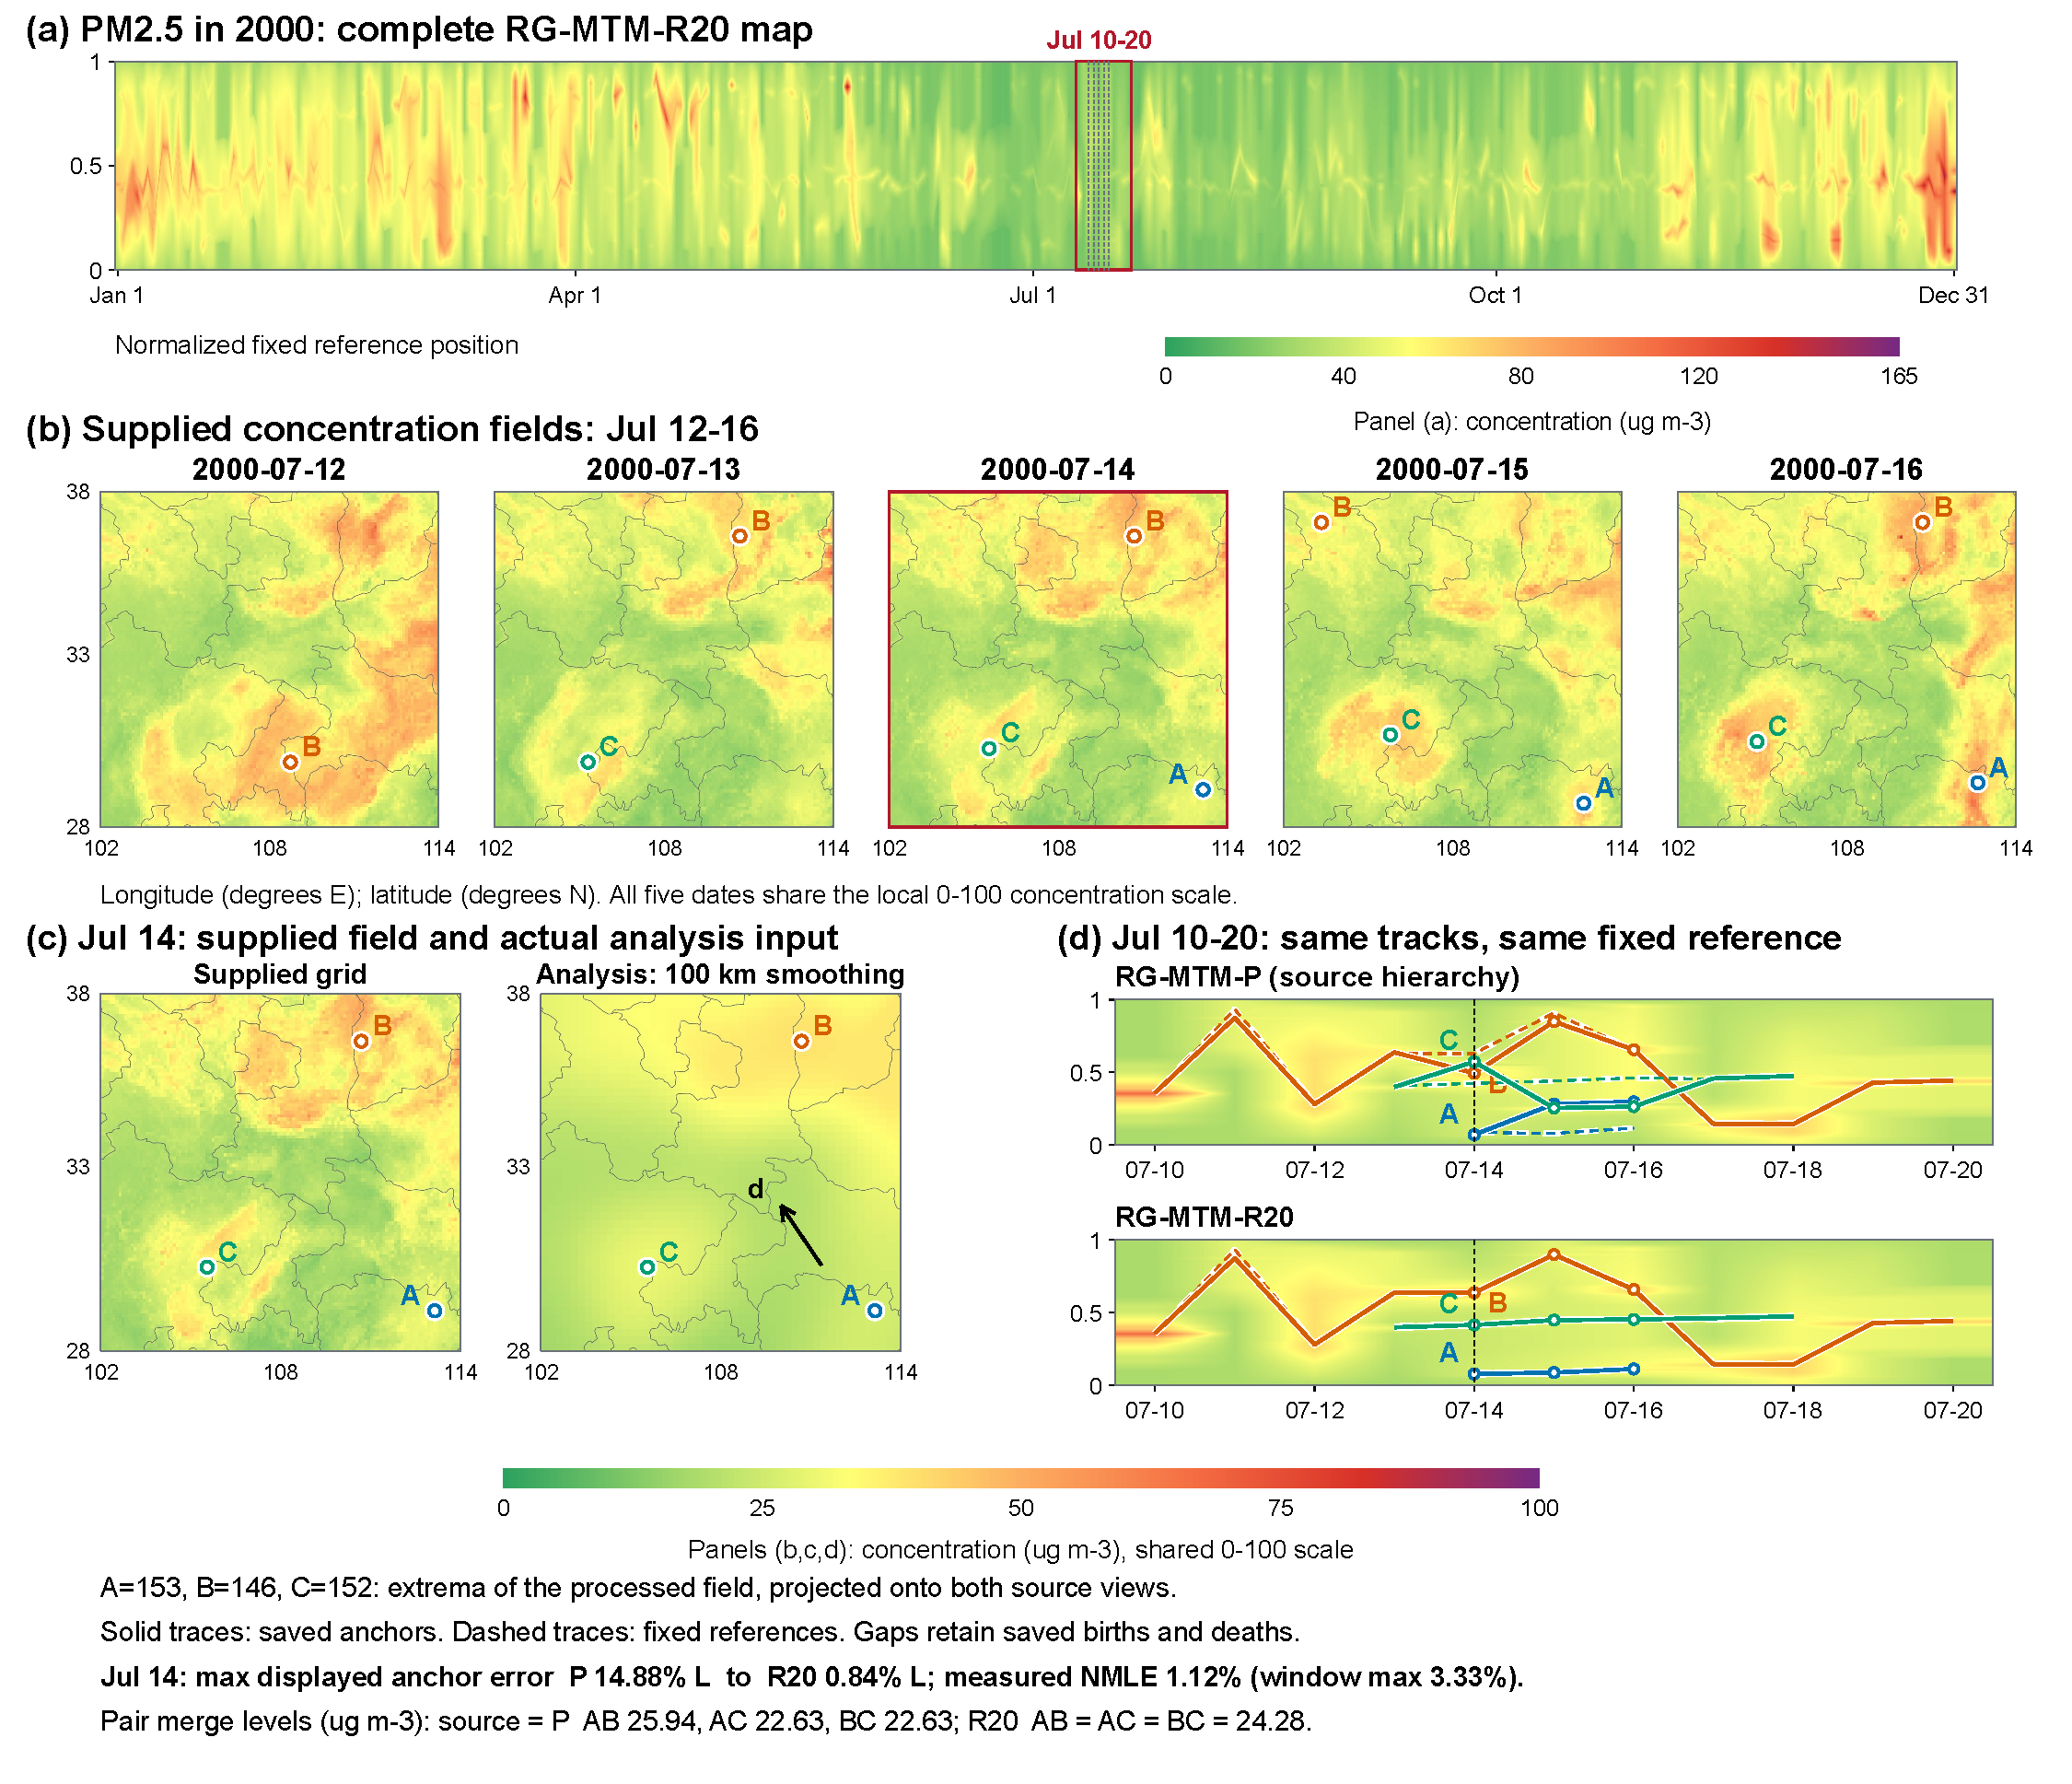
\includegraphics[width=\textwidth]{figures/Fig13.pdf}
\caption{PM2.5: complete-year context and a source-linked July case. (a) All 366 R20 profiles with July 10--20 outlined. (b) Supplied concentration fields for July 12--16, with geographic context from Natural Earth~\cite{NaturalEarth:Admin1}. (c) July 14 supplied and processed fields; markers show the same processed extrema $A=153,B=146,C=152$, and $d$ is the fixed annual reference direction. (d) Complete P/R20 profiles over July 10--20, with solid saved anchors and dashed fixed references. Tracks retain their saved births and deaths. Panel (a) uses 0--165\,$\mu$g\,m$^{-3}$; panels (b)--(d) share 0--100\,$\mu$g\,m$^{-3}$ without per-date rescaling. At July 14, maximum displayed-anchor displacement falls from 14.88\% to 0.84\% of $L$, at 1.12\% measured NMLE; the window's maximum NMLE is 3.33\%. This is a selected mechanism witness, not a claim of annual motion improvement. Display interpolation preserves every saved profile.}
\label{fig:pm25_case}
\end{figure*}

Figure~\ref{fig:pm25_case} connects the annual map to supplied concentration fields and the actual processed input. The geographic views retain the same 102--114\textdegree E, 28--38\textdegree N window; the analysis uses the existing $49\times49$ grid and fixed 100\,km smoothing and documented boundary treatment. The supplied grid and processed field are shown separately so that extracted extrema are not mistaken for independent observations or validated pollution objects.

For reproducible selection, we retain frames whose strongest three-feature interleaving witness exceeds $0.02L$ and whose three tracks coexist for at least three consecutive saved dates. Five of 34 witness frames satisfy the continuity condition. The frame closest to their median witness obstruction is July 14 (frame 195), with tracks $A=153,B=146,C=152$ continuing through July 16. Selection uses obstruction and continuity, rather than motion accuracy or achieved positional gain. Supplement S8 records the full candidate list and coordinate checks.

On July 14, the source hierarchy joins $A,B$ before $C$, while the fixed reference orders them $A,C,B$. P places $A,B,C$, and R20 uses $A,C,B$. From July 14 to 15, $C$'s reference increases by only $1.62\%L$, but its displayed P anchor decreases by $31.84\%L$ as the hierarchy-compatible arrangement changes. R20 increases by $3.27\%L$, following the reference direction. These are single-anchor changes, separate from the pairwise motion-error metric. The source views and dashed references distinguish a layout jump from a change in the processed extremum's projected position.

The positional gain has a measurable scalar price. On July 14, source/P connection levels are 25.9364\,$\mu$g\,m$^{-3}$ for $A/B$ and 22.6261\,$\mu$g\,m$^{-3}$ for either outside pair. R20 sets all three to 24.2813\,$\mu$g\,m$^{-3}$. The resulting worst-pair change is 1.6552\,$\mu$g\,m$^{-3}$, or 1.12\% of the fixed annual processed range; the local window reaches 3.33\% NMLE. This case explains a mechanism without overturning the annual comparison: P makes 42/95 motion errors and R20 makes 47/95. The tracked extrema do not establish pollutant transport, emission attribution, or the identity of a named haze episode.

\subsection{Relaxation Eligibility and Measured Cost}
\begin{figure*}[t]
\centering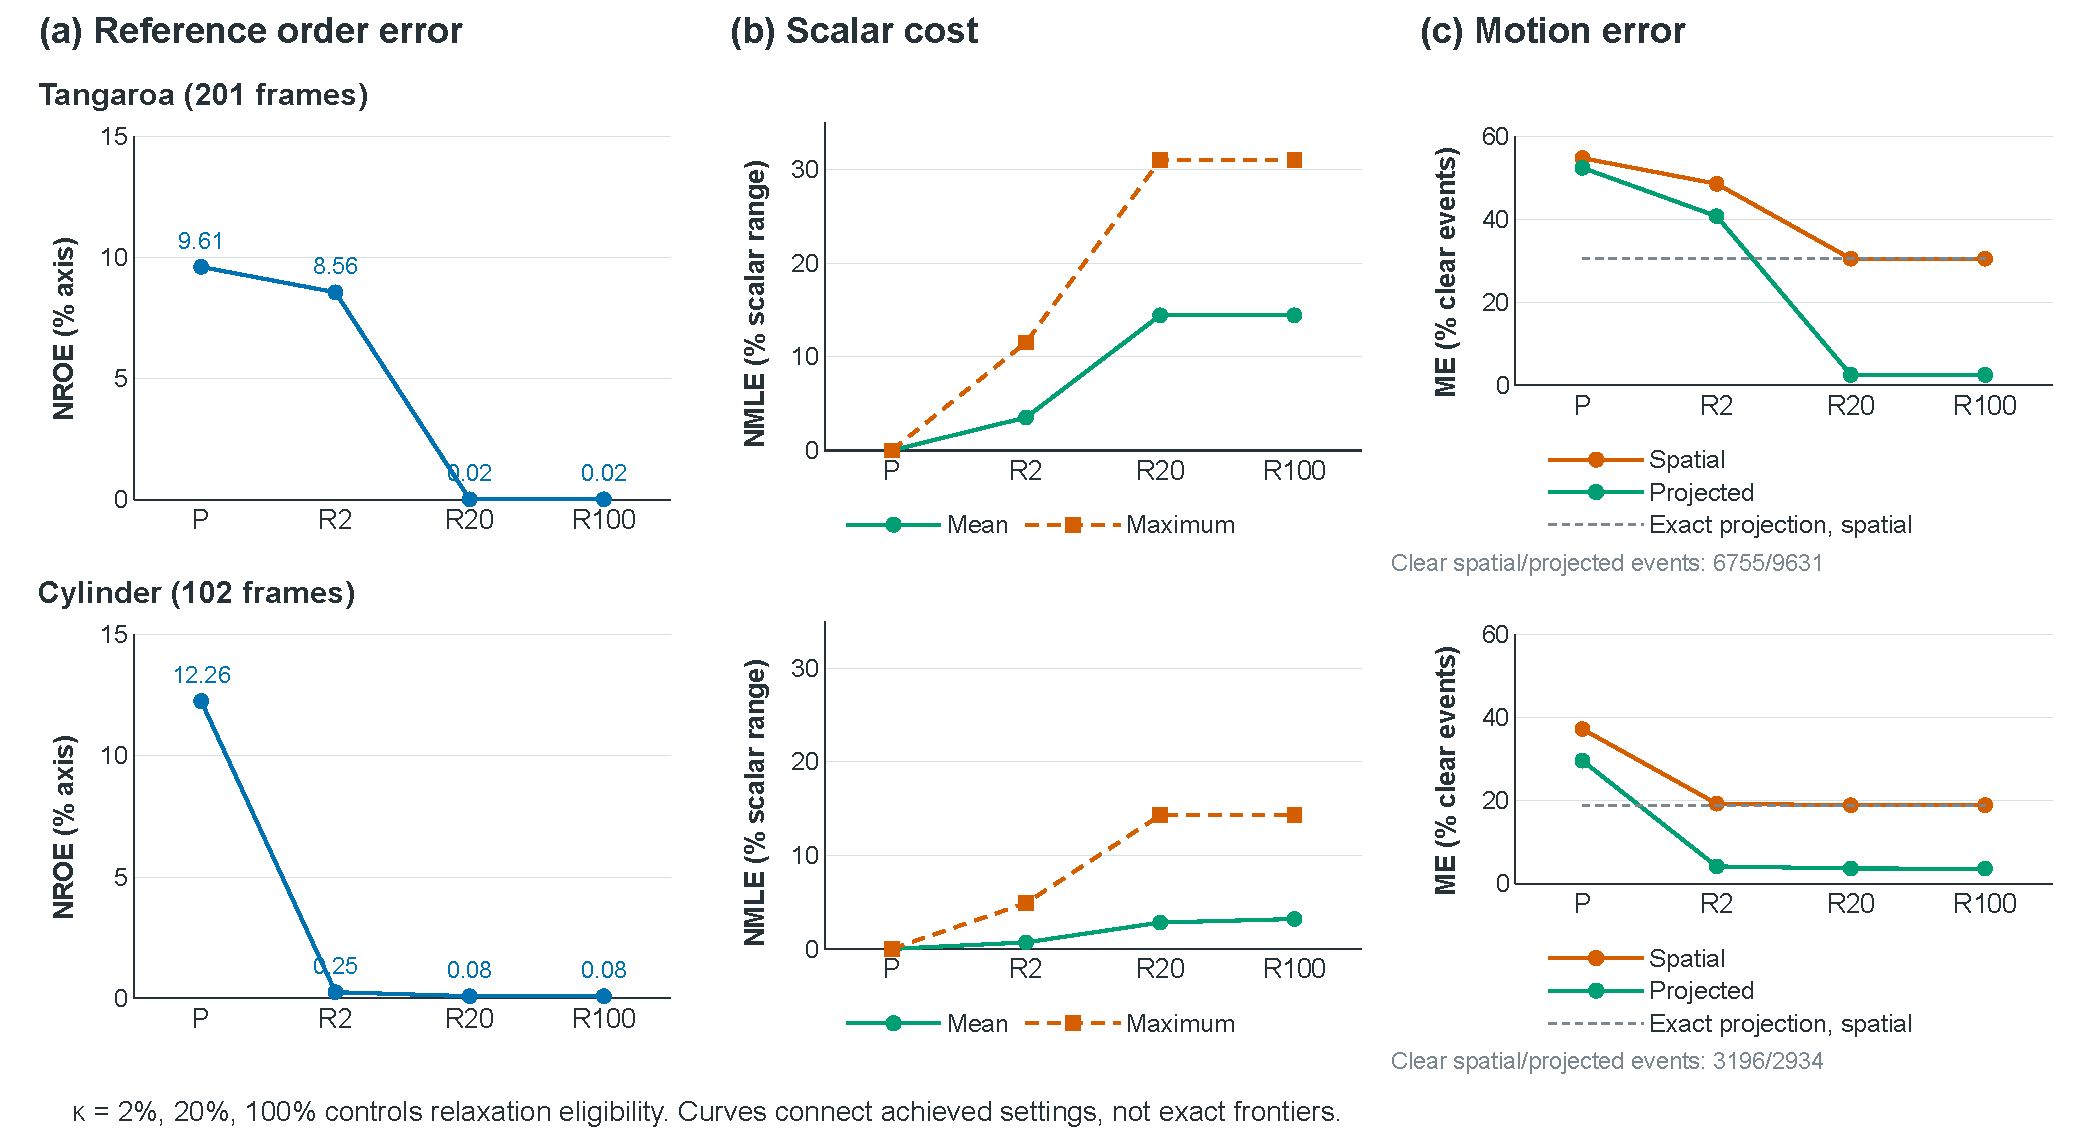
\includegraphics[width=\textwidth]{figures/Fig14.pdf}
\caption{Eligibility and measured position--scalar trade-offs on Tangaroa and Cylinder. Saved P, R2, R20, and R100 outputs share each dataset's source fields and persistence. NROE and NMLE are independently measured; $\kappa$ selects eligible parent gaps rather than capping output error. Larger settings need not improve both quantities: Tangaroa R20/R100 coincide, while Cylinder R100 matches R20's order error with greater mean scalar cost. These large-tree operating points do not form an exhaustive exact frontier.}
\label{fig:eligibility_tradeoff}
\end{figure*}

Figure~\ref{fig:eligibility_tradeoff} compares P, R2, R20 and R100 on the same complete Tangaroa and Cylinder inputs. The threshold $\kappa$ selects eligible parent gaps; it is not a bound on the measured output NMLE. Tangaroa R20 and R100 coincide. Cylinder R100 retains R20's mean NROE while increasing mean NMLE from 2.810\% to 3.190\%. The grey exact-projection reference uses its own clear-event population and supplies a diagnostic, rather than a universal lower bound on spatial-motion error. These operating points complement the exhaustive small-tree frontiers without claiming exhaustive enumeration for the larger trees.

\subsubsection{Planar Budget Response Across Time}
\begin{figure*}[t]
\centering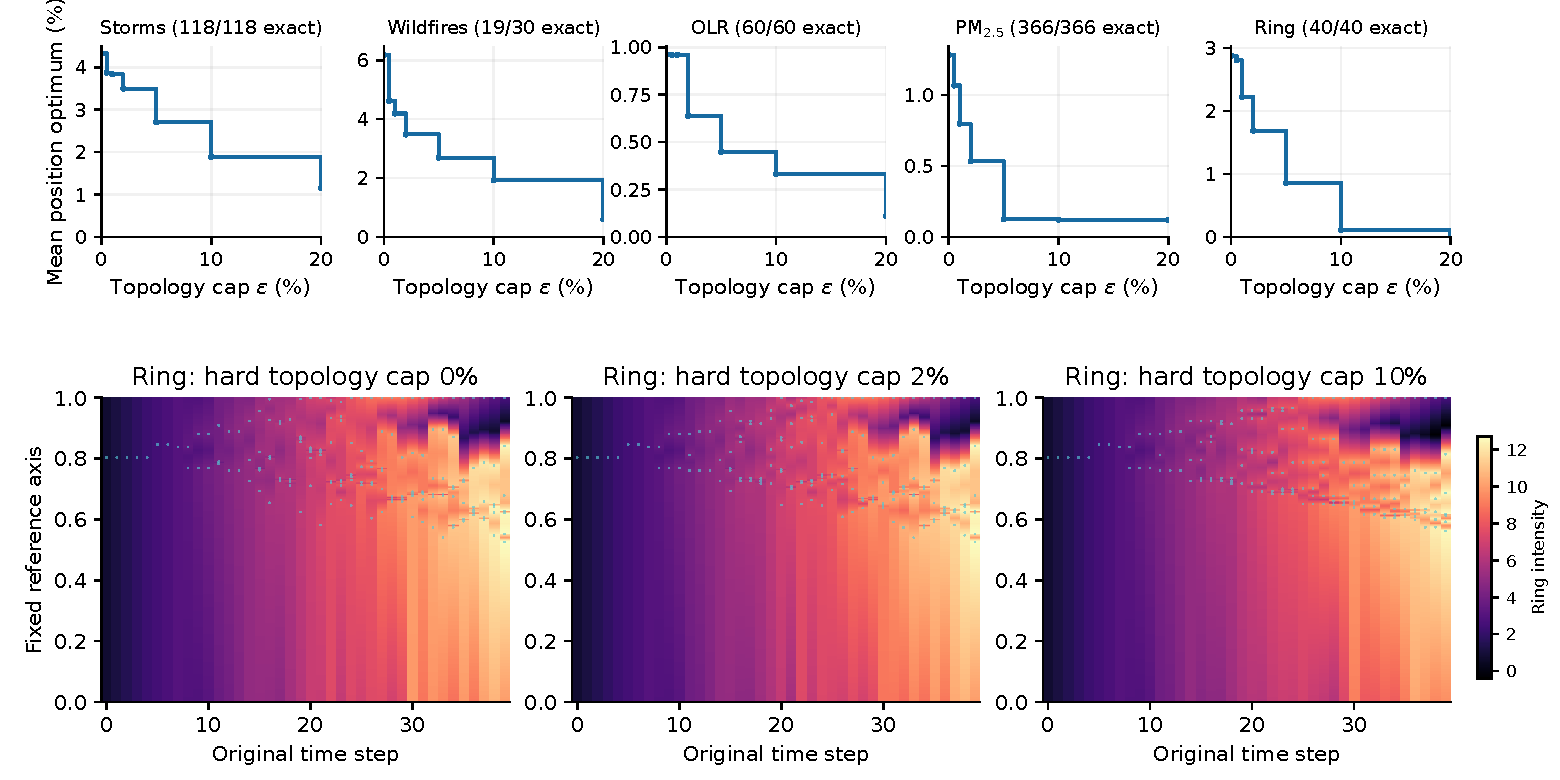
\includegraphics[width=\textwidth]{figures/Fig15.pdf}
\caption{New hard-budget family experiments. Top: temporal means of framewise minimax reference error against a true labelled topology-error cap; titles disclose exhaustive coverage. Wildfires includes 11 candidate-only upper bounds, using the same pool at every cap. Bottom: Ring scalar witness maps at 0\%, 2\% and 10\% topology allowances, with LP anchors in cyan and the same scalar colour scale. These piecewise-linear barrier witnesses illustrate changing admissible orders; they do not reconstruct source fields or establish temporal smoothness. The plotted rasters are illustrative; continuous saved anchors and barriers supply the budget checks.}
\label{fig:budget_response}
\end{figure*}
The threshold system changes which orders can be displayed, rather than merely changing a weighted objective. Small allowances retain expensive order conflicts; larger allowances admit additional orders until a frame reaches the free-packing regime or the best order in the declared candidate pool. The Ring maps illustrate the selected LP witnesses across the original 40 fields. Their framewise selection can change between columns; a smooth temporal solution requires an explicitly specified secondary policy within the budgets. The earlier R2/R20/R100 curves describe another construction policy, not these hard topology caps.

\subsection{Operating Regimes and Two-Budget Maps}\label{sec:unified_maps}
\begin{figure*}[t]
\centering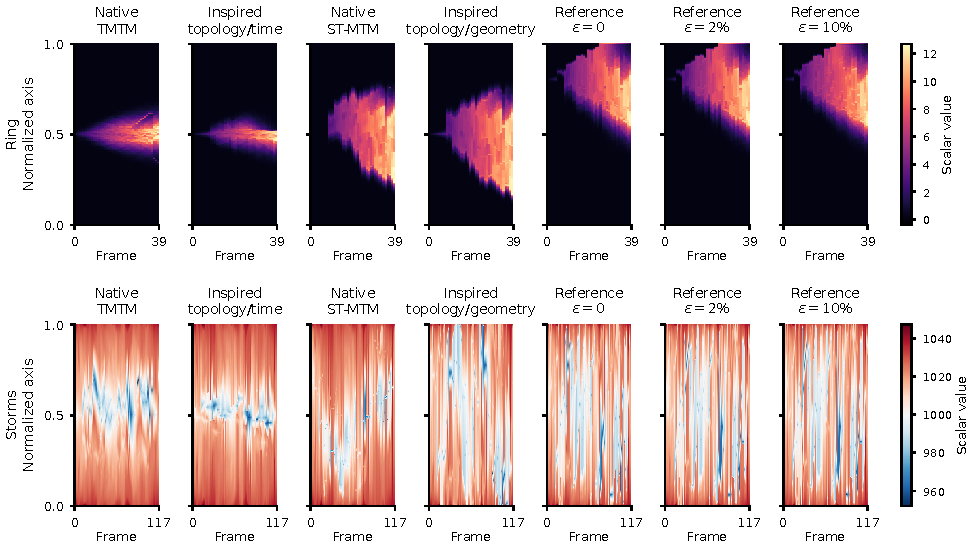
\includegraphics[width=\linewidth]{figures/Fig16.pdf}
\caption{Native methods and operating regimes of one model on Ring (top) and Storms (bottom). Within each row all columns use the same fields, time steps and scalar colours; the colour range includes corrected barrier values, which are constructed values rather than source observations. Columns 2, 4 and 5--7 share interval widths, canvas, QP and renderer; only the controls change. Native methods use their own layouts and scalar filling. All display axes are normalized to $[0,1]$; one global native reflection follows the similarity fit, with no per-frame warping. The topology/time and topology/geometry columns express inspired design principles, not native-output equality. All reference columns use $B=\infty$ and vary the true topology allowance.}\label{fig:unified_regimes}
\end{figure*}

\begin{figure*}[t]
\centering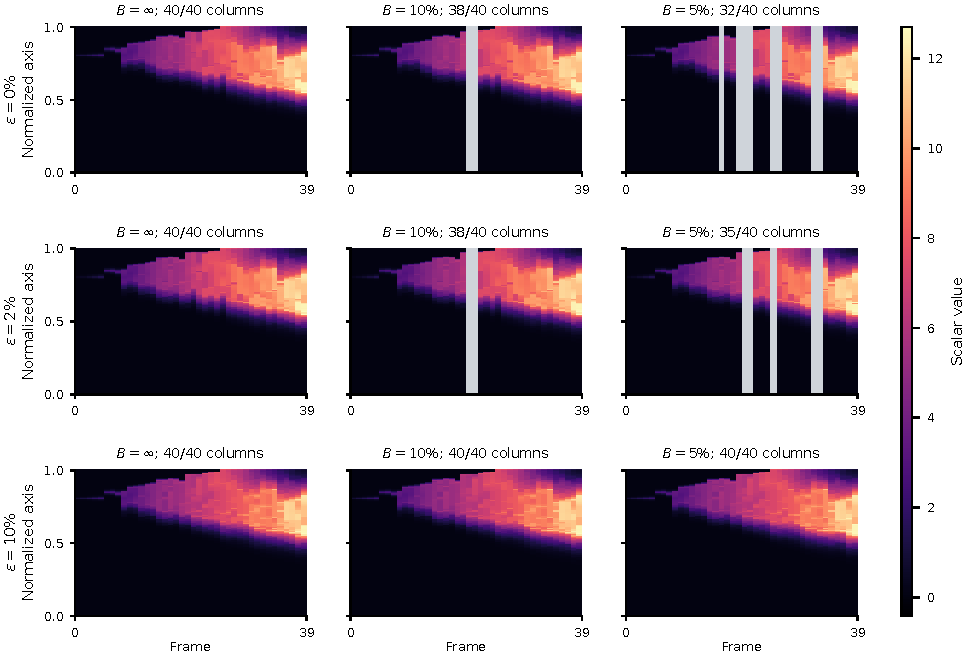
\includegraphics[width=\linewidth]{figures/Fig17.pdf}
\caption{Ring maps across topology allowances (rows) and reference-position caps (columns), using the same reference-guided objective, candidate pool and scalar renderer. Position allowances are fractions of the common canvas; topology allowances are fractions of the fixed scalar range. Gray columns denote frames for which no candidate meets both budgets, not zero scalar values. A history restarts after such a missing frame. Counts report witnessed feasible columns, rather than full-space feasibility on candidate-only frames. Finite maps include measured strict-extremum clearance and anchor rounding, which are separate from the continuous constraints.}\label{fig:unified_budget_grid}
\end{figure*}

The operating-regime views expose the difference between a topology-preserving temporal emphasis, a relative-distance emphasis, and an absolute reference target. They also show why output resemblance must be measured rather than inferred from the name of a regime. The native methods allocate widths and arrange internal samples differently. The common-model columns deliberately retain one representation so that changes can be attributed to the declared controls. The two-budget matrix additionally makes incompatible requests visible as missing witnesses instead of silently widening a tolerance.

% Keep all Results figures and tables ahead of the closing discussion.
\FloatBarrier
\section{Discussion and Limitations}\label{sec:discussion}
\subsection{Interpreting Reference Alignment}
Common-model operating regimes and descriptive native-output similarity address RQ1; certificates and forward/inverse feasibility queries address RQ2. The tested reference-order gains extend across planar and volumetric inputs, while motion and geometry gains depend on the reference and event population (RQ3). Nucleon's unchanged P/R profiles show that useful alignment need not require relaxation.

A band's movement combines projected source movement and changes in its anchor-to-reference residual. Wildfires frames 17--19 show a fixed reference accompanying a shifting P anchor; matched source views separate these effects. For volumetric fields, the reference compresses two further spatial dimensions, so similar projected positions can represent features far apart in the source domain.

The new common-model experiment compares design principles directly within one representation. It also reveals their limits: native-output resemblance varies by input, with substantially weaker Storms ST-MTM agreement than Ring. The anchor-level temporal surrogate omits all-subtree overlap and uses shared absolute widths, so it should not be interpreted as an implementation substitute for either native method.

Reference alignment complements distance preservation and temporal coherence. On OLR, P/R motion-proxy errors remain 3/56 despite improved order, and ST-MTM retains better SNS, TW, and TD on Storms, OLR, and PM2.5. Annual PM2.5 has 95 clear events at the primary thresholds, with 42 P errors and 47 R20 errors. These outcomes preclude treating a lower NROE as a general guarantee of better geometry, motion interpretation, or reader performance. The motion-margin result in Supplement S1 instead certifies projected distance changes when achieved anchor errors are sufficiently small.

\subsection{Choosing Preferences and Error Budgets}
A user selects the relations to emphasize within the common interval model. Setting reference and geometry weights to zero, disabling the position cap and using a stationary temporal target gives topology--time alignment. Enabling centroid stress gives topology--geometry preservation. Reference guidance activates absolute targets and projected motion; a scalar allowance determines how much merge-level change can be spent to resolve order conflict. These regimes share one construction. Native TMTM and ST-MTM remain independent baselines with different sample allocation and width rules, so a shared design principle does not establish output identity. An application can prescribe either error cap or ask the inverse query for the allowance required by a position tolerance.

RG-MTM-P is appropriate when source merge thresholds must remain intact. Its position certificate quantifies the displacement that the chosen geometry and hierarchy permit, while its actual anchor errors disclose the result of the budgeted secondary layout. RG-MTM-R adds reference-compatible orders while retaining the extrema and their values. Each relaxed output should be read together with its achieved displacement and mean and maximum merge-level errors; sequence means alone can conceal a large local scalar change.

The eligibility parameter $\kappa$ bounds adjacent parent gaps of nodes that may be flattened. It is neither birth--death persistence nor an output-distortion tolerance. Wider eligibility need not improve the measured trade-off: Cylinder R100 has the same mean NROE as R20 but greater mean NMLE. The new RG-MTM-B specialization imposes that tolerance on continuous fixed-order costs and rejects inadmissible candidates. Its 603 exhaustive frames supply exact optima; 11 candidate-only frames supply feasible upper bounds. Strict-extremum raster output still needs explicit clearance and actual-error acceptance checks. The retained large-tree eligibility construction supplies separate temporal maps, not the new hard-budget guarantee.

Relaxation changes regular scalar values and connection thresholds. The negative Wildfires connections are artificial filling values, even though the source fire observations are nonnegative. Merge-level error describes these changed pairwise thresholds, while retaining extremum values; it does not establish preservation of scalar distributions, thresholded areas, or every internal feature. An analysis that depends on a physical threshold should consult the source field and the displayed barrier before drawing a conclusion from the relaxed map.

\subsection{Scope of the Evidence}
Spatial projection and preprocessing determine the structures represented by the map. Tangaroa's direction captures 57.686\% of matched motion energy; exact projected anchors still produce 2060/6755 three-dimensional motion-proxy errors. Cylinder's exact $x$ projection likewise retains 603/3196 errors. These controls locate a limit of the chosen reference even when positional layout error vanishes. Multiple references could expose additional spatial relations, but are outside the present evaluation.

New budget experiments use the same 614 planar frames but construct new LP/barrier witnesses; they do not reuse previous temporal scores as measurements of those witnesses. The reported populations answer different questions. The 614-frame suite compares four methods on common planar temporal inputs. The 64-frame mirror-motion control isolates absolute anchoring. Tangaroa and Cylinder test independent original-grid volumetric inputs; Nucleon tests one static slice; reconstructed Benzene tests section coherence in a declared classical potential. The 744-hour Storms overview supplies a denser visualization and is excluded from the 118-frame quantitative sequence. These populations are not combined into an overall accuracy score. ST-MTM was not run on the static additions or volumetric sequences.

Input correspondence is imperfect. Tangaroa has 2459/6925 boundary-touching supports and 36--186 derived nodes (reference: 50--186). Cylinder uses 102 public volumes rather than the reported 508 frames. Benzene is a reconstructed potential; annual PM2.5 replaces an exploratory January sample. These declared protocols support the reported comparisons, not exact reproduction of every original input or untested generalization.

Overlap matches provide computational correspondences rather than validated physical tracks. Source-provider event calendars give temporal context rather than cyclone identities, and the Cylinder proxies do not establish vortex labels. Independent physical-track validation and studies of how readers interpret the maps remain necessary extensions. Further persistence settings, internal-feature evaluation, additional scalar models, and preregistered task-specific comparisons would broaden the evidence.

\subsection{Computational Limits and Future Work}
Fixed-order position costs and non-strict barriers are exact within the model; complete enumeration yields exact frontiers. The common solver evaluates every admitted candidate, while the retained large-tree construction uses brackets and at most four QPs. Both can leave search gaps. Finer previews do not strengthen numerical evidence.

Future work includes richer overlap-aware temporal terms, scalable search, sequence-wide optimization and verified raster acceptance. Historical planar QPs may fall back to LP-feasible layouts; their optimality and end-to-end timing need further assessment. The ST-MTM SciPy OLO heuristic exceeds the exhaustive adjacency minimum in eight of 148 audited frames, qualifying the declared reimplementation rather than every original setting.

\section{Conclusion}\label{sec:conclusion}
RG-MTM makes the conflict between hierarchical feature grouping and fixed spatial reference positions explicit. Its positional certificates separate packing and boundary cost from the displacement imposed by subtree contiguity. Optimal fixed-order filling preserves extremum values and quantifies the minimum labelled merge-level cost of a changed order. The preserving and relaxed constructions turn this analysis into scalar maps whose achieved anchor and barrier errors can be inspected alongside the source fields.

The five-sequence planar evaluation, independent reference control, original-grid Tangaroa and Cylinder sequences, static Nucleon slice, and reconstructed Benzene sections show the reference alignment gained under their declared protocols and the scalar connectivity exchanged for it. The resulting maps support comparisons along a fixed reference while making the limits of projection, hierarchy, and scalar filling visible and measurable.

\section*{Acknowledgments}
OpenAI Codex assisted manuscript editing, figure/evidence code, and earlier experiment orchestration. We thank the ERA5, FRP, OLR, PM2.5, Natural Earth, and Tangaroa providers. We also acknowledge the square-cylinder simulation by Camarri, Salvetti, Buffoni, and Iollo and its uniform resampling by Tino Weinkauf, and the public Inviwo molecular geometry used in the Benzene reconstruction.
% Results floats have already been drained; let references follow the text.
\begingroup
\interlinepenalty=10000
\setlength{\bibspacing}{-0.3pt}
\bibliographystyle{abbrv-doi-narrow}
\bibliography{refs}
\endgroup
\end{document}
